% =====================================================================
%  Issue register and activity timeline, LSSTCam operations 2025
%  Companion to the 2025 chronology (appendix); intended for CTN-007.
%
%  Derived from the Rubin Observatory Slack channels #cam-summit-ops and
%  #cam-operator (2025-01-01 to 2025-12-31, top-level messages and all
%  thread replies).  "Active" means the issue was being discussed or
%  worked on in those channels; an issue may have been settled elsewhere
%  (Jira, e-mail, in person) without that showing here.
%
%  Preamble requirements: tikz, xcolor, graphicx, booktabs.
%
%  Revision 4 (author review):
%    - GLY-02 retired -> PCS-01 (reliability) and PCS-02 (restart difficulty,
%      plus the MRCR failure tracked as LSSTCAM-119); glycol and the PCS
%      chiller are now separate categories
%    - CCS-04 split: the vacuum-gauge interlock fault stays there, the general
%      silent death of periodic tasks becomes CCS-08
%    - MEC-01 split: sheared pancake-wrap bolts (closed) stay there, the camera
%      door charging becomes MEC-04 (grounding strap being implemented)
%    - FP-04 is an accepted, unrepairable defect; FP-06 is tracked in
%      #cam-issues-esd; DAQ-01 notes the serial console (IHS-9431); DAQ-02
%      names the affected host
%
%  Revision 3: dormant folded into open; FW-01 resolved by the 0x313a5014
%    firmware; CCS-07 renamed to Kafka broker; SHT-02 evidence made explicit.
%
%  Revision 2 (author review):
%    - DYN-03 retired  -> CCS-05 (protective logic is a control-system defect)
%    - NET-01 retired  -> CCS-06 (jGroups storms)
%    - NET-02 retired  -> CCS-07 (broker / rebpower memory exhaustion)
%    - FP-06 added: REB power-supply trips suspected to be ESD, split out of MEC-01
%    - "Hx"/"hex" read as the camera heat exchanger, not the hexapod
%    - cross-references added to CRYO-01, FP-01, FP-02, SHT-01, SHT-02
%    - issues open at year end now run to the end of the timeline
% =====================================================================

% Ticket / document link macros (harmless if already defined).
\providecommand{\rubintkt}[1]{\href{https://rubinobs.atlassian.net/browse/#1}{#1}}
\providecommand{\slactkt}[1]{\href{https://jira.slac.stanford.edu/browse/#1}{#1}}
\providecommand{\lsstls}[1]{\href{https://ls.st/#1}{#1}}
\definecolor{stres}{HTML}{2E7D32}
\definecolor{stmit}{HTML}{1565A0}
\definecolor{stwrk}{HTML}{6A3D9A}
\definecolor{stopn}{HTML}{C0392B}
\definecolor{stdor}{HTML}{8A6D1F}
\definecolor{sttra}{HTML}{00695C}
\definecolor{issspan}{HTML}{C8CDD2}
\definecolor{issgrid}{HTML}{E4E7EA}

\subsection{Issue register and activity timeline, 2025 to the storm of July 2026}
\label{sec:issues}

This section organizes the LSSTCam operations record by
\emph{problem}: each recurring or distinct issue is given an identifier,
summarized once, and placed on a timeline showing when it was actually being
worked on.  It runs from January 2025 to 13~July 2026, when the summit was
closed ahead of the storm; the storm and the recovery from it are the subject
of a separate document.  The date-ordered account it is drawn from is
reproduced in Appendix~\ref{sec:chronology}.  The purpose of the organization is to
separate three categories of issues that a chronology conflates --- issues that were closed,
issues that the observatory learned to live with, and issues that were never
closed at all.

Identifiers carry a category prefix: \texttt{CRYO} (cryogenic refrigeration), \texttt{DYN} (dynalene [utility-trunk cooling]), \texttt{GLY} (glycol [facility cooling]), \texttt{PCS} (Pumped-coolant system chiller), \texttt{PWR} (site power), \texttt{AIR} (compressed dry air), \texttt{FP} (focal plane), \texttt{FW} (rEB firmware), \texttt{DAQ} (data acquisition), \texttt{CCS} (Camera Control System), \texttt{SHT} (shutter), \texttt{FES} (filter exchange system), \texttt{OPT} (stray light), \texttt{MEC} (mechanical and integration), \texttt{IT} (Summit IT), \texttt{VAC} (cryostat vacuum).
Status is assigned based on the evidence of the operations channels, using five
categories:

\begin{center}
\begin{tabular}{@{}clp{10.2cm}@{}}
\textcolor{stres}{\textbf{R}} & Resolved & Cause found and fixed, no recurrence in the logs \\
\textcolor{stmit}{\textbf{M}} & Mitigated & Recurrence contained by a procedure or design change, mechanism unchanged \\
\textcolor{stwrk}{\textbf{W}} & Workaround & Operated around a known defect that was never repaired \\
\textcolor{stopn}{\textbf{O}} & Open & Not closed: still active or recurring at the end of the period, or never resolved and no longer being mentioned \\
\textcolor{sttra}{\textbf{T}} & Transferred & Handed to another group and tracked outside LSSTCam operations \\
\end{tabular}
\end{center}

\noindent
Four entries are also marked with a ``\textbf{?}''.  In those cases the record stops before
the outcome is entered, so the classification has to be settled from sources outside
these channels; the summary says in each case what is missing.

\begin{table}[htb]
\centering
\begin{tabular}{llr}
\toprule
 & Status & Issues \\
\midrule
\textcolor{stres}{\textbf{R}} & Resolved & 11 \\
\textcolor{stmit}{\textbf{M}} & Mitigated & 14 \\
\textcolor{stwrk}{\textbf{W}} & Workaround & 9 \\
\textcolor{stopn}{\textbf{O}} & Open & 26 \\
\textcolor{sttra}{\textbf{T}} & Transferred & 2 \\
\midrule
 & \textbf{Total} & \textbf{62} \\
\bottomrule
\end{tabular}
\caption{Status of the 62 issues identified in the LSSTCam operations
channels between January 2025 and July 2026.  Open covers both ends of a spectrum: issues that were still
generating traffic in July 2026, and issues that were never closed and simply
stopped being mentioned --- the timeline of
Figure~\ref{fig:issue-timeline} distinguishes the two, since the latter show a
long tail with no activity.  Those, together with the nine Workaround issues, are the
entries most likely to need a decision and action.}
\label{tab:issue-status}
\end{table}
\begin{figure}[htbp]
\centering
\begingroup\hypersetup{hidelinks}%
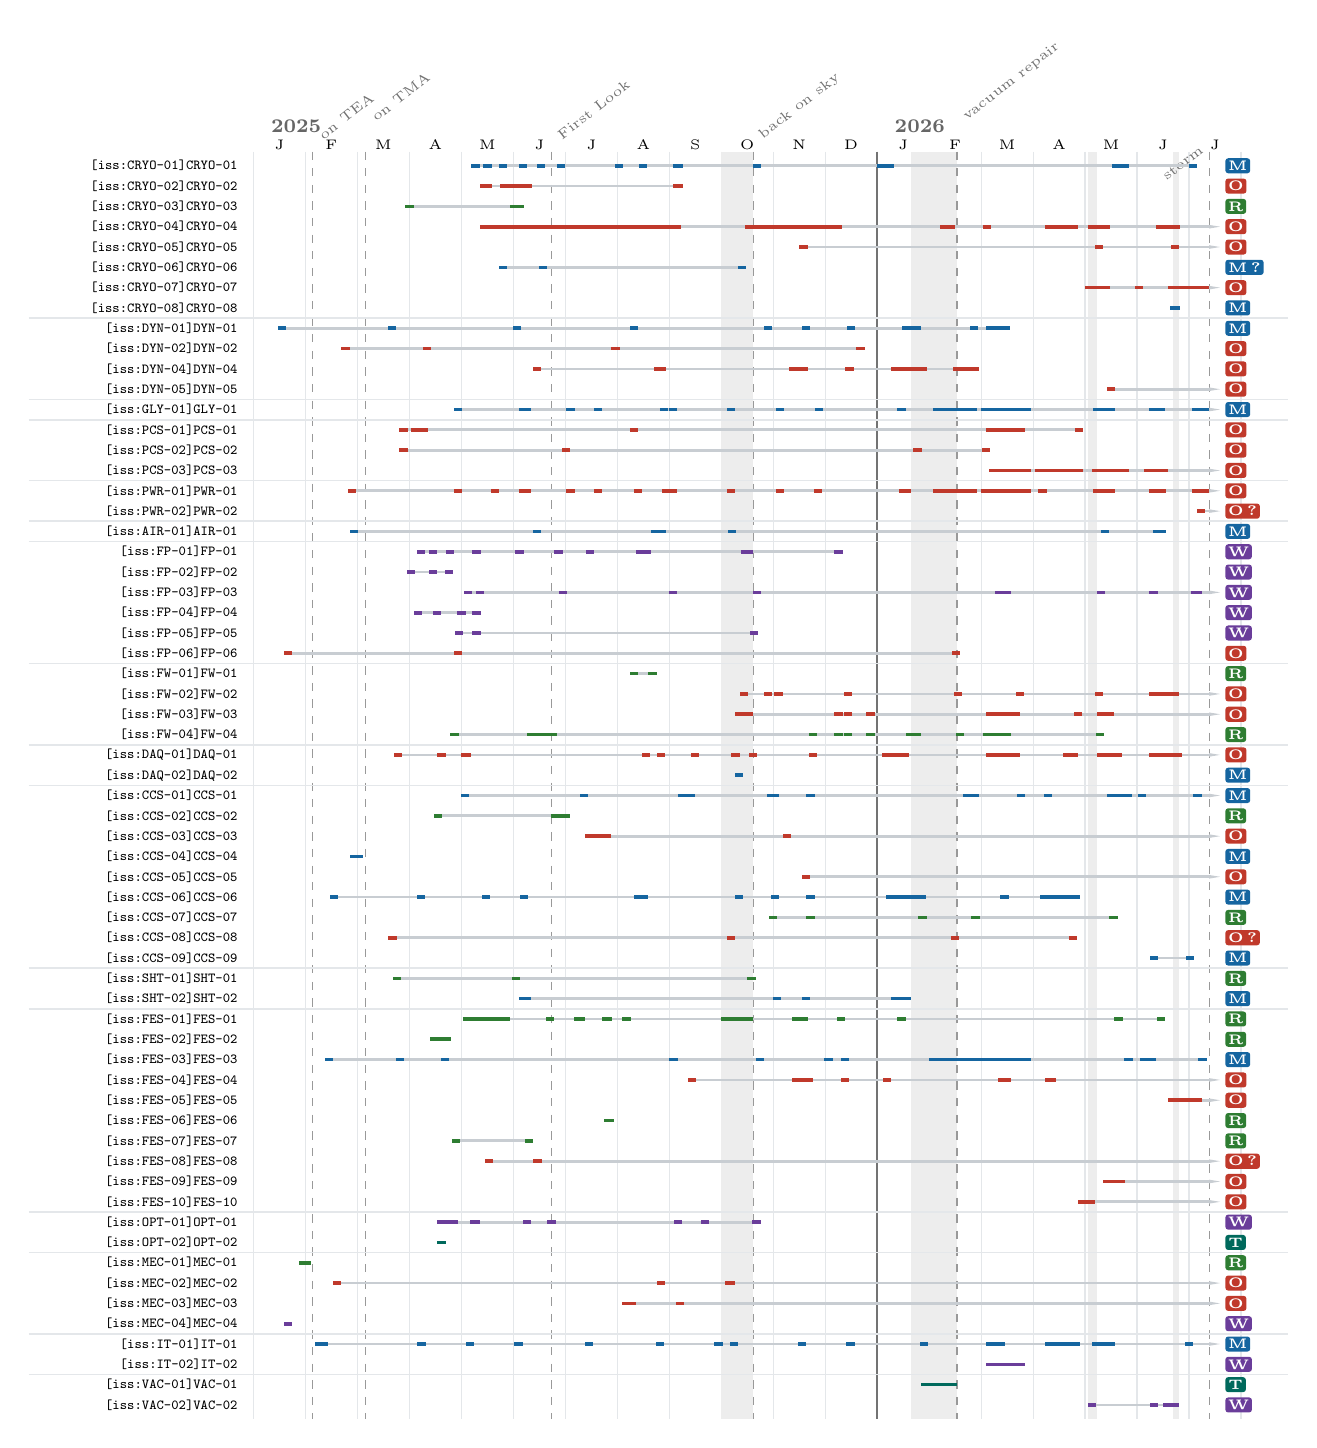
\begin{tikzpicture}[x=0.660cm, y=-0.258cm]
\foreach \m in {0,1,...,19} { \draw[issgrid,line width=0.4pt] (\m,-0.7) -- (\m,61.70); }
\node[font=\tiny] at (0.500,-1.05) {J};
\node[font=\tiny] at (1.500,-1.05) {F};
\node[font=\tiny] at (2.500,-1.05) {M};
\node[font=\tiny] at (3.500,-1.05) {A};
\node[font=\tiny] at (4.500,-1.05) {M};
\node[font=\tiny] at (5.500,-1.05) {J};
\node[font=\tiny] at (6.500,-1.05) {J};
\node[font=\tiny] at (7.500,-1.05) {A};
\node[font=\tiny] at (8.500,-1.05) {S};
\node[font=\tiny] at (9.500,-1.05) {O};
\node[font=\tiny] at (10.500,-1.05) {N};
\node[font=\tiny] at (11.500,-1.05) {D};
\node[font=\tiny] at (12.500,-1.05) {J};
\node[font=\tiny] at (13.500,-1.05) {F};
\node[font=\tiny] at (14.500,-1.05) {M};
\node[font=\tiny] at (15.500,-1.05) {A};
\node[font=\tiny] at (16.500,-1.05) {M};
\node[font=\tiny] at (17.500,-1.05) {J};
\node[font=\tiny] at (18.500,-1.05) {J};
\draw[black!55,line width=0.7pt] (12,-0.7) -- (12,61.70);
\node[font=\scriptsize\bfseries,text=black!60,anchor=west] at (0.15,-1.95) {2025};
\node[font=\scriptsize\bfseries,text=black!60,anchor=west] at (12.15,-1.95) {2026};
\fill[black!7] (9.000,-0.7) rectangle (9.613,61.70);
\fill[black!7] (12.645,-0.7) rectangle (13.536,61.70);
\fill[black!7] (16.065,-0.7) rectangle (16.226,61.70);
\fill[black!7] (17.700,-0.7) rectangle (17.800,61.70);
\draw[black!40,dashed,line width=0.4pt] (1.143,-0.7) -- (1.143,61.70);
\node[font=\tiny,text=black!55,anchor=west,rotate=38] at (1.143,-1.15) {on TEA};
\draw[black!40,dashed,line width=0.4pt] (2.161,-0.7) -- (2.161,61.70);
\node[font=\tiny,text=black!55,anchor=west,rotate=38] at (2.161,-2.05) {on TMA};
\draw[black!40,dashed,line width=0.4pt] (5.733,-0.7) -- (5.733,61.70);
\node[font=\tiny,text=black!55,anchor=west,rotate=38] at (5.733,-1.15) {First Look};
\draw[black!40,dashed,line width=0.4pt] (9.613,-0.7) -- (9.613,61.70);
\node[font=\tiny,text=black!55,anchor=west,rotate=38] at (9.613,-1.15) {back on sky};
\draw[black!40,dashed,line width=0.4pt] (13.536,-0.7) -- (13.536,61.70);
\node[font=\tiny,text=black!55,anchor=west,rotate=38] at (13.536,-2.05) {vacuum repair};
\draw[black!40,dashed,line width=0.4pt] (18.387,-0.7) -- (18.387,61.70);
\node[font=\tiny,text=black!55,anchor=east,rotate=38] at (18.387,-1.15) {storm};
\node[font=\tiny\ttfamily,anchor=east] at (-0.121,0.00) {\hyperref[iss:CRYO-01]{CRYO-01}};
\draw[issspan,line width=1.0pt] (4.226,0.00) -- (18.161,0.00);
\fill[stmit] (4.194,-0.09) rectangle (4.354,0.09);
\fill[stmit] (4.420,-0.09) rectangle (4.580,0.09);
\fill[stmit] (4.726,-0.09) rectangle (4.886,0.09);
\fill[stmit] (5.103,-0.09) rectangle (5.263,0.09);
\fill[stmit] (5.453,-0.09) rectangle (5.613,0.09);
\fill[stmit] (5.837,-0.09) rectangle (5.997,0.09);
\fill[stmit] (6.952,-0.09) rectangle (7.112,0.09);
\fill[stmit] (7.420,-0.09) rectangle (7.580,0.09);
\fill[stmit] (8.067,-0.09) rectangle (8.267,0.09);
\fill[stmit] (9.613,-0.09) rectangle (9.774,0.09);
\fill[stmit] (12.000,-0.09) rectangle (12.323,0.09);
\fill[stmit] (16.516,-0.09) rectangle (16.839,0.09);
\fill[stmit] (18.000,-0.09) rectangle (18.161,0.09);
\node[font=\tiny\bfseries,text=white,fill=stmit,rounded corners=1pt,inner sep=1.0pt,minimum width=0.26cm,anchor=west] at (18.690,0.00) {M};
\node[font=\tiny\ttfamily,anchor=east] at (-0.121,1.00) {\hyperref[iss:CRYO-02]{CRYO-02}};
\draw[issspan,line width=1.0pt] (4.355,1.00) -- (8.267,1.00);
\fill[stopn] (4.355,0.91) rectangle (4.581,1.09);
\fill[stopn] (4.742,0.91) rectangle (5.367,1.09);
\fill[stopn] (8.067,0.91) rectangle (8.267,1.09);
\node[font=\tiny\bfseries,text=white,fill=stopn,rounded corners=1pt,inner sep=1.0pt,minimum width=0.26cm,anchor=west] at (18.690,1.00) {O};
\node[font=\tiny\ttfamily,anchor=east] at (-0.121,2.00) {\hyperref[iss:CRYO-03]{CRYO-03}};
\draw[issspan,line width=1.0pt] (3.000,2.00) -- (5.200,2.00);
\fill[stres] (2.920,1.91) rectangle (3.080,2.09);
\fill[stres] (4.935,1.91) rectangle (5.200,2.09);
\node[font=\tiny\bfseries,text=white,fill=stres,rounded corners=1pt,inner sep=1.0pt,minimum width=0.26cm,anchor=west] at (18.690,2.00) {R};
\node[font=\tiny\ttfamily,anchor=east] at (-0.121,3.00) {\hyperref[iss:CRYO-04]{CRYO-04}};
\draw[issspan,line width=1.0pt] (4.355,3.00) -- (18.387,3.00);
\fill[issspan] (18.387,2.91) -- (18.387,3.09) -- (18.599,3.00) -- cycle;
\fill[stopn] (4.355,2.91) rectangle (8.233,3.09);
\fill[stopn] (9.452,2.91) rectangle (11.323,3.09);
\fill[stopn] (13.214,2.91) rectangle (13.500,3.09);
\fill[stopn] (14.033,2.91) rectangle (14.193,3.09);
\fill[stopn] (15.233,2.91) rectangle (15.867,3.09);
\fill[stopn] (16.065,2.91) rectangle (16.484,3.09);
\fill[stopn] (17.367,2.91) rectangle (17.833,3.09);
\node[font=\tiny\bfseries,text=white,fill=stopn,rounded corners=1pt,inner sep=1.0pt,minimum width=0.26cm,anchor=west] at (18.690,3.00) {O};
\node[font=\tiny\ttfamily,anchor=east] at (-0.121,4.00) {\hyperref[iss:CRYO-05]{CRYO-05}};
\draw[issspan,line width=1.0pt] (10.567,4.00) -- (18.387,4.00);
\fill[issspan] (18.387,3.91) -- (18.387,4.09) -- (18.599,4.00) -- cycle;
\fill[stopn] (10.503,3.91) rectangle (10.663,4.09);
\fill[stopn] (16.194,3.91) rectangle (16.354,4.09);
\fill[stopn] (17.653,3.91) rectangle (17.813,4.09);
\node[font=\tiny\bfseries,text=white,fill=stopn,rounded corners=1pt,inner sep=1.0pt,minimum width=0.26cm,anchor=west] at (18.690,4.00) {O};
\node[font=\tiny\ttfamily,anchor=east] at (-0.121,5.00) {\hyperref[iss:CRYO-06]{CRYO-06}};
\draw[issspan,line width=1.0pt] (4.806,5.00) -- (9.484,5.00);
\fill[stmit] (4.726,4.91) rectangle (4.886,5.09);
\fill[stmit] (5.487,4.91) rectangle (5.647,5.09);
\fill[stmit] (9.323,4.91) rectangle (9.484,5.09);
\node[font=\tiny\bfseries,text=white,fill=stmit,rounded corners=1pt,inner sep=1.0pt,minimum width=0.26cm,anchor=west] at (18.690,5.00) {M\,?};
\node[font=\tiny\ttfamily,anchor=east] at (-0.121,6.00) {\hyperref[iss:CRYO-07]{CRYO-07}};
\draw[issspan,line width=1.0pt] (16.000,6.00) -- (18.387,6.00);
\fill[issspan] (18.387,5.91) -- (18.387,6.09) -- (18.599,6.00) -- cycle;
\fill[stopn] (16.000,5.91) rectangle (16.484,6.09);
\fill[stopn] (16.953,5.91) rectangle (17.113,6.09);
\fill[stopn] (17.600,5.91) rectangle (18.387,6.09);
\node[font=\tiny\bfseries,text=white,fill=stopn,rounded corners=1pt,inner sep=1.0pt,minimum width=0.26cm,anchor=west] at (18.690,6.00) {O};
\node[font=\tiny\ttfamily,anchor=east] at (-0.121,7.00) {\hyperref[iss:CRYO-08]{CRYO-08}};
\draw[issspan,line width=1.0pt] (17.633,7.00) -- (17.833,7.00);
\fill[stmit] (17.633,6.91) rectangle (17.833,7.09);
\node[font=\tiny\bfseries,text=white,fill=stmit,rounded corners=1pt,inner sep=1.0pt,minimum width=0.26cm,anchor=west] at (18.690,7.00) {M};
\draw[issgrid,line width=0.6pt] (-4.33,7.50) -- (19.90,7.50);
\node[font=\tiny\ttfamily,anchor=east] at (-0.121,8.00) {\hyperref[iss:DYN-01]{DYN-01}};
\draw[issspan,line width=1.0pt] (0.548,8.00) -- (14.548,8.00);
\fill[stmit] (0.468,7.91) rectangle (0.628,8.09);
\fill[stmit] (2.581,7.91) rectangle (2.741,8.09);
\fill[stmit] (4.987,7.91) rectangle (5.147,8.09);
\fill[stmit] (7.243,7.91) rectangle (7.403,8.09);
\fill[stmit] (9.823,7.91) rectangle (9.983,8.09);
\fill[stmit] (10.553,7.91) rectangle (10.713,8.09);
\fill[stmit] (11.420,7.91) rectangle (11.580,8.09);
\fill[stmit] (12.484,7.91) rectangle (12.839,8.09);
\fill[stmit] (13.777,7.91) rectangle (13.937,8.09);
\fill[stmit] (14.097,7.91) rectangle (14.548,8.09);
\node[font=\tiny\bfseries,text=white,fill=stmit,rounded corners=1pt,inner sep=1.0pt,minimum width=0.26cm,anchor=west] at (18.690,8.00) {M};
\node[font=\tiny\ttfamily,anchor=east] at (-0.121,9.00) {\hyperref[iss:DYN-02]{DYN-02}};
\draw[issspan,line width=1.0pt] (1.714,9.00) -- (11.677,9.00);
\fill[stopn] (1.688,8.91) rectangle (1.848,9.09);
\fill[stopn] (3.253,8.91) rectangle (3.413,9.09);
\fill[stopn] (6.888,8.91) rectangle (7.048,9.09);
\fill[stopn] (11.597,8.91) rectangle (11.757,9.09);
\node[font=\tiny\bfseries,text=white,fill=stopn,rounded corners=1pt,inner sep=1.0pt,minimum width=0.26cm,anchor=west] at (18.690,9.00) {O};
\node[font=\tiny\ttfamily,anchor=east] at (-0.121,10.00) {\hyperref[iss:DYN-04]{DYN-04}};
\draw[issspan,line width=1.0pt] (5.433,10.00) -- (13.964,10.00);
\fill[stopn] (5.370,9.91) rectangle (5.530,10.09);
\fill[stopn] (7.710,9.91) rectangle (7.935,10.09);
\fill[stopn] (10.300,9.91) rectangle (10.667,10.09);
\fill[stopn] (11.388,9.91) rectangle (11.548,10.09);
\fill[stopn] (12.258,9.91) rectangle (12.968,10.09);
\fill[stopn] (13.464,9.91) rectangle (13.964,10.09);
\node[font=\tiny\bfseries,text=white,fill=stopn,rounded corners=1pt,inner sep=1.0pt,minimum width=0.26cm,anchor=west] at (18.690,10.00) {O};
\node[font=\tiny\ttfamily,anchor=east] at (-0.121,11.00) {\hyperref[iss:DYN-05]{DYN-05}};
\draw[issspan,line width=1.0pt] (16.419,11.00) -- (18.387,11.00);
\fill[issspan] (18.387,10.91) -- (18.387,11.09) -- (18.599,11.00) -- cycle;
\fill[stopn] (16.419,10.91) rectangle (16.581,11.09);
\node[font=\tiny\bfseries,text=white,fill=stopn,rounded corners=1pt,inner sep=1.0pt,minimum width=0.26cm,anchor=west] at (18.690,11.00) {O};
\draw[issgrid,line width=0.6pt] (-4.33,11.50) -- (19.90,11.50);
\node[font=\tiny\ttfamily,anchor=east] at (-0.121,12.00) {\hyperref[iss:GLY-01]{GLY-01}};
\draw[issspan,line width=1.0pt] (3.900,12.00) -- (18.387,12.00);
\fill[issspan] (18.387,11.91) -- (18.387,12.09) -- (18.599,12.00) -- cycle;
\fill[stmit] (3.853,11.91) rectangle (4.013,12.09);
\fill[stmit] (5.100,11.91) rectangle (5.333,12.09);
\fill[stmit] (6.017,11.91) rectangle (6.177,12.09);
\fill[stmit] (6.549,11.91) rectangle (6.709,12.09);
\fill[stmit] (7.823,11.91) rectangle (7.983,12.09);
\fill[stmit] (7.987,11.91) rectangle (8.147,12.09);
\fill[stmit] (9.114,11.91) rectangle (9.274,12.09);
\fill[stmit] (10.053,11.91) rectangle (10.213,12.09);
\fill[stmit] (10.803,11.91) rectangle (10.963,12.09);
\fill[stmit] (12.388,11.91) rectangle (12.548,12.09);
\fill[stmit] (13.071,11.91) rectangle (13.929,12.09);
\fill[stmit] (14.000,11.91) rectangle (14.968,12.09);
\fill[stmit] (16.161,11.91) rectangle (16.581,12.09);
\fill[stmit] (17.233,11.91) rectangle (17.533,12.09);
\fill[stmit] (18.065,11.91) rectangle (18.387,12.09);
\node[font=\tiny\bfseries,text=white,fill=stmit,rounded corners=1pt,inner sep=1.0pt,minimum width=0.26cm,anchor=west] at (18.690,12.00) {M};
\draw[issgrid,line width=0.6pt] (-4.33,12.50) -- (19.90,12.50);
\node[font=\tiny\ttfamily,anchor=east] at (-0.121,13.00) {\hyperref[iss:PCS-01]{PCS-01}};
\draw[issspan,line width=1.0pt] (2.871,13.00) -- (15.967,13.00);
\fill[stopn] (2.807,12.91) rectangle (2.967,13.09);
\fill[stopn] (3.037,12.91) rectangle (3.197,13.09);
\fill[stopn] (3.203,12.91) rectangle (3.363,13.09);
\fill[stopn] (7.243,12.91) rectangle (7.403,13.09);
\fill[stopn] (14.097,12.91) rectangle (14.839,13.09);
\fill[stopn] (15.800,12.91) rectangle (15.967,13.09);
\node[font=\tiny\bfseries,text=white,fill=stopn,rounded corners=1pt,inner sep=1.0pt,minimum width=0.26cm,anchor=west] at (18.690,13.00) {O};
\node[font=\tiny\ttfamily,anchor=east] at (-0.121,14.00) {\hyperref[iss:PCS-02]{PCS-02}};
\draw[issspan,line width=1.0pt] (2.871,14.00) -- (14.097,14.00);
\fill[stopn] (2.807,13.91) rectangle (2.967,14.09);
\fill[stopn] (5.936,13.91) rectangle (6.096,14.09);
\fill[stopn] (12.694,13.91) rectangle (12.854,14.09);
\fill[stopn] (14.017,13.91) rectangle (14.177,14.09);
\node[font=\tiny\bfseries,text=white,fill=stopn,rounded corners=1pt,inner sep=1.0pt,minimum width=0.26cm,anchor=west] at (18.690,14.00) {O};
\node[font=\tiny\ttfamily,anchor=east] at (-0.121,15.00) {\hyperref[iss:PCS-03]{PCS-03}};
\draw[issspan,line width=1.0pt] (14.161,15.00) -- (18.387,15.00);
\fill[issspan] (18.387,14.91) -- (18.387,15.09) -- (18.599,15.00) -- cycle;
\fill[stopn] (14.161,14.91) rectangle (14.968,15.09);
\fill[stopn] (15.033,14.91) rectangle (15.967,15.09);
\fill[stopn] (16.129,14.91) rectangle (16.839,15.09);
\fill[stopn] (17.133,14.91) rectangle (17.600,15.09);
\node[font=\tiny\bfseries,text=white,fill=stopn,rounded corners=1pt,inner sep=1.0pt,minimum width=0.26cm,anchor=west] at (18.690,15.00) {O};
\draw[issgrid,line width=0.6pt] (-4.33,15.50) -- (19.90,15.50);
\node[font=\tiny\ttfamily,anchor=east] at (-0.121,16.00) {\hyperref[iss:PWR-01]{PWR-01}};
\draw[issspan,line width=1.0pt] (1.857,16.00) -- (18.387,16.00);
\fill[issspan] (18.387,15.91) -- (18.387,16.09) -- (18.599,16.00) -- cycle;
\fill[stopn] (1.813,15.91) rectangle (1.973,16.09);
\fill[stopn] (3.853,15.91) rectangle (4.013,16.09);
\fill[stopn] (4.565,15.91) rectangle (4.725,16.09);
\fill[stopn] (5.100,15.91) rectangle (5.333,16.09);
\fill[stopn] (6.017,15.91) rectangle (6.177,16.09);
\fill[stopn] (6.549,15.91) rectangle (6.709,16.09);
\fill[stopn] (7.323,15.91) rectangle (7.484,16.09);
\fill[stopn] (7.855,15.91) rectangle (8.015,16.09);
\fill[stopn] (7.987,15.91) rectangle (8.147,16.09);
\fill[stopn] (9.114,15.91) rectangle (9.274,16.09);
\fill[stopn] (10.053,15.91) rectangle (10.213,16.09);
\fill[stopn] (10.787,15.91) rectangle (10.947,16.09);
\fill[stopn] (12.419,15.91) rectangle (12.645,16.09);
\fill[stopn] (13.071,15.91) rectangle (13.929,16.09);
\fill[stopn] (14.000,15.91) rectangle (14.968,16.09);
\fill[stopn] (15.103,15.91) rectangle (15.263,16.09);
\fill[stopn] (16.161,15.91) rectangle (16.581,16.09);
\fill[stopn] (17.233,15.91) rectangle (17.567,16.09);
\fill[stopn] (18.065,15.91) rectangle (18.387,16.09);
\node[font=\tiny\bfseries,text=white,fill=stopn,rounded corners=1pt,inner sep=1.0pt,minimum width=0.26cm,anchor=west] at (18.690,16.00) {O};
\node[font=\tiny\ttfamily,anchor=east] at (-0.121,17.00) {\hyperref[iss:PWR-02]{PWR-02}};
\draw[issspan,line width=1.0pt] (18.194,17.00) -- (18.387,17.00);
\fill[issspan] (18.387,16.91) -- (18.387,17.09) -- (18.599,17.00) -- cycle;
\fill[stopn] (18.146,16.91) rectangle (18.306,17.09);
\node[font=\tiny\bfseries,text=white,fill=stopn,rounded corners=1pt,inner sep=1.0pt,minimum width=0.26cm,anchor=west] at (18.690,17.00) {O\,?};
\draw[issgrid,line width=0.6pt] (-4.33,17.50) -- (19.90,17.50);
\node[font=\tiny\ttfamily,anchor=east] at (-0.121,18.00) {\hyperref[iss:AIR-01]{AIR-01}};
\draw[issspan,line width=1.0pt] (1.929,18.00) -- (17.567,18.00);
\fill[stmit] (1.849,17.91) rectangle (2.009,18.09);
\fill[stmit] (5.370,17.91) rectangle (5.530,18.09);
\fill[stmit] (7.645,17.91) rectangle (7.935,18.09);
\fill[stmit] (9.130,17.91) rectangle (9.290,18.09);
\fill[stmit] (16.307,17.91) rectangle (16.467,18.09);
\fill[stmit] (17.300,17.91) rectangle (17.567,18.09);
\node[font=\tiny\bfseries,text=white,fill=stmit,rounded corners=1pt,inner sep=1.0pt,minimum width=0.26cm,anchor=west] at (18.690,18.00) {M};
\draw[issgrid,line width=0.6pt] (-4.33,18.50) -- (19.90,18.50);
\node[font=\tiny\ttfamily,anchor=east] at (-0.121,19.00) {\hyperref[iss:FP-01]{FP-01}};
\draw[issspan,line width=1.0pt] (3.200,19.00) -- (11.290,19.00);
\fill[stwrk] (3.137,18.91) rectangle (3.297,19.09);
\fill[stwrk] (3.370,18.91) rectangle (3.530,19.09);
\fill[stwrk] (3.703,18.91) rectangle (3.863,19.09);
\fill[stwrk] (4.210,18.91) rectangle (4.370,19.09);
\fill[stwrk] (5.037,18.91) rectangle (5.197,19.09);
\fill[stwrk] (5.787,18.91) rectangle (5.947,19.09);
\fill[stwrk] (6.388,18.91) rectangle (6.548,19.09);
\fill[stwrk] (7.355,18.91) rectangle (7.645,19.09);
\fill[stwrk] (9.387,18.91) rectangle (9.613,19.09);
\fill[stwrk] (11.178,18.91) rectangle (11.338,19.09);
\node[font=\tiny\bfseries,text=white,fill=stwrk,rounded corners=1pt,inner sep=1.0pt,minimum width=0.26cm,anchor=west] at (18.690,19.00) {W};
\node[font=\tiny\ttfamily,anchor=east] at (-0.121,20.00) {\hyperref[iss:FP-02]{FP-02}};
\draw[issspan,line width=1.0pt] (3.033,20.00) -- (3.767,20.00);
\fill[stwrk] (2.953,19.91) rectangle (3.113,20.09);
\fill[stwrk] (3.370,19.91) rectangle (3.530,20.09);
\fill[stwrk] (3.687,19.91) rectangle (3.847,20.09);
\node[font=\tiny\bfseries,text=white,fill=stwrk,rounded corners=1pt,inner sep=1.0pt,minimum width=0.26cm,anchor=west] at (18.690,20.00) {W};
\node[font=\tiny\ttfamily,anchor=east] at (-0.121,21.00) {\hyperref[iss:FP-03]{FP-03}};
\draw[issspan,line width=1.0pt] (4.129,21.00) -- (18.387,21.00);
\fill[issspan] (18.387,20.91) -- (18.387,21.09) -- (18.599,21.00) -- cycle;
\fill[stwrk] (4.049,20.91) rectangle (4.209,21.09);
\fill[stwrk] (4.275,20.91) rectangle (4.435,21.09);
\fill[stwrk] (5.870,20.91) rectangle (6.030,21.09);
\fill[stwrk] (7.987,20.91) rectangle (8.147,21.09);
\fill[stwrk] (9.613,20.91) rectangle (9.774,21.09);
\fill[stwrk] (14.258,20.91) rectangle (14.581,21.09);
\fill[stwrk] (16.226,20.91) rectangle (16.386,21.09);
\fill[stwrk] (17.233,20.91) rectangle (17.400,21.09);
\fill[stwrk] (18.032,20.91) rectangle (18.258,21.09);
\node[font=\tiny\bfseries,text=white,fill=stwrk,rounded corners=1pt,inner sep=1.0pt,minimum width=0.26cm,anchor=west] at (18.690,21.00) {W};
\node[font=\tiny\ttfamily,anchor=east] at (-0.121,22.00) {\hyperref[iss:FP-04]{FP-04}};
\draw[issspan,line width=1.0pt] (3.167,22.00) -- (4.290,22.00);
\fill[stwrk] (3.087,21.91) rectangle (3.247,22.09);
\fill[stwrk] (3.453,21.91) rectangle (3.613,22.09);
\fill[stwrk] (3.920,21.91) rectangle (4.080,22.09);
\fill[stwrk] (4.210,21.91) rectangle (4.370,22.09);
\node[font=\tiny\bfseries,text=white,fill=stwrk,rounded corners=1pt,inner sep=1.0pt,minimum width=0.26cm,anchor=west] at (18.690,22.00) {W};
\node[font=\tiny\ttfamily,anchor=east] at (-0.121,23.00) {\hyperref[iss:FP-05]{FP-05}};
\draw[issspan,line width=1.0pt] (3.933,23.00) -- (9.645,23.00);
\fill[stwrk] (3.870,22.91) rectangle (4.030,23.09);
\fill[stwrk] (4.210,22.91) rectangle (4.370,23.09);
\fill[stwrk] (9.549,22.91) rectangle (9.709,23.09);
\node[font=\tiny\bfseries,text=white,fill=stwrk,rounded corners=1pt,inner sep=1.0pt,minimum width=0.26cm,anchor=west] at (18.690,23.00) {W};
\node[font=\tiny\ttfamily,anchor=east] at (-0.121,24.00) {\hyperref[iss:FP-06]{FP-06}};
\draw[issspan,line width=1.0pt] (0.645,24.00) -- (13.536,24.00);
\fill[stopn] (0.581,23.91) rectangle (0.741,24.09);
\fill[stopn] (3.853,23.91) rectangle (4.013,24.09);
\fill[stopn] (13.438,23.91) rectangle (13.598,24.09);
\node[font=\tiny\bfseries,text=white,fill=stopn,rounded corners=1pt,inner sep=1.0pt,minimum width=0.26cm,anchor=west] at (18.690,24.00) {O};
\draw[issgrid,line width=0.6pt] (-4.33,24.50) -- (19.90,24.50);
\node[font=\tiny\ttfamily,anchor=east] at (-0.121,25.00) {\hyperref[iss:FW-01]{FW-01}};
\draw[issspan,line width=1.0pt] (7.323,25.00) -- (7.710,25.00);
\fill[stres] (7.243,24.91) rectangle (7.403,25.09);
\fill[stres] (7.597,24.91) rectangle (7.757,25.09);
\node[font=\tiny\bfseries,text=white,fill=stres,rounded corners=1pt,inner sep=1.0pt,minimum width=0.26cm,anchor=west] at (18.690,25.00) {R};
\node[font=\tiny\ttfamily,anchor=east] at (-0.121,26.00) {\hyperref[iss:FW-02]{FW-02}};
\draw[issspan,line width=1.0pt] (9.387,26.00) -- (18.387,26.00);
\fill[issspan] (18.387,25.91) -- (18.387,26.09) -- (18.599,26.00) -- cycle;
\fill[stopn] (9.355,25.91) rectangle (9.515,26.09);
\fill[stopn] (9.823,25.91) rectangle (9.983,26.09);
\fill[stopn] (10.020,25.91) rectangle (10.180,26.09);
\fill[stopn] (11.355,25.91) rectangle (11.515,26.09);
\fill[stopn] (13.474,25.91) rectangle (13.634,26.09);
\fill[stopn] (14.662,25.91) rectangle (14.822,26.09);
\fill[stopn] (16.194,25.91) rectangle (16.354,26.09);
\fill[stopn] (17.233,25.91) rectangle (17.800,26.09);
\node[font=\tiny\bfseries,text=white,fill=stopn,rounded corners=1pt,inner sep=1.0pt,minimum width=0.26cm,anchor=west] at (18.690,26.00) {O};
\node[font=\tiny\ttfamily,anchor=east] at (-0.121,27.00) {\hyperref[iss:FW-03]{FW-03}};
\draw[issspan,line width=1.0pt] (9.258,27.00) -- (18.387,27.00);
\fill[issspan] (18.387,26.91) -- (18.387,27.09) -- (18.599,27.00) -- cycle;
\fill[stopn] (9.258,26.91) rectangle (9.613,27.09);
\fill[stopn] (11.178,26.91) rectangle (11.338,27.09);
\fill[stopn] (11.355,26.91) rectangle (11.515,27.09);
\fill[stopn] (11.791,26.91) rectangle (11.951,27.09);
\fill[stopn] (14.097,26.91) rectangle (14.742,27.09);
\fill[stopn] (15.787,26.91) rectangle (15.947,27.09);
\fill[stopn] (16.226,26.91) rectangle (16.548,27.09);
\node[font=\tiny\bfseries,text=white,fill=stopn,rounded corners=1pt,inner sep=1.0pt,minimum width=0.26cm,anchor=west] at (18.690,27.00) {O};
\node[font=\tiny\ttfamily,anchor=east] at (-0.121,28.00) {\hyperref[iss:FW-04]{FW-04}};
\draw[issspan,line width=1.0pt] (3.833,28.00) -- (16.323,28.00);
\fill[stres] (3.787,27.91) rectangle (3.947,28.09);
\fill[stres] (5.267,27.91) rectangle (5.833,28.09);
\fill[stres] (10.687,27.91) rectangle (10.847,28.09);
\fill[stres] (11.178,27.91) rectangle (11.338,28.09);
\fill[stres] (11.355,27.91) rectangle (11.515,28.09);
\fill[stres] (11.791,27.91) rectangle (11.951,28.09);
\fill[stres] (12.548,27.91) rectangle (12.839,28.09);
\fill[stres] (13.509,27.91) rectangle (13.669,28.09);
\fill[stres] (14.032,27.91) rectangle (14.581,28.09);
\fill[stres] (16.210,27.91) rectangle (16.370,28.09);
\node[font=\tiny\bfseries,text=white,fill=stres,rounded corners=1pt,inner sep=1.0pt,minimum width=0.26cm,anchor=west] at (18.690,28.00) {R};
\draw[issgrid,line width=0.6pt] (-4.33,28.50) -- (19.90,28.50);
\node[font=\tiny\ttfamily,anchor=east] at (-0.121,29.00) {\hyperref[iss:DAQ-01]{DAQ-01}};
\draw[issspan,line width=1.0pt] (2.742,29.00) -- (18.387,29.00);
\fill[issspan] (18.387,28.91) -- (18.387,29.09) -- (18.599,29.00) -- cycle;
\fill[stopn] (2.694,28.91) rectangle (2.854,29.09);
\fill[stopn] (3.537,28.91) rectangle (3.697,29.09);
\fill[stopn] (4.000,28.91) rectangle (4.194,29.09);
\fill[stopn] (7.468,28.91) rectangle (7.628,29.09);
\fill[stopn] (7.759,28.91) rectangle (7.919,29.09);
\fill[stopn] (8.420,28.91) rectangle (8.580,29.09);
\fill[stopn] (9.194,28.91) rectangle (9.354,29.09);
\fill[stopn] (9.533,28.91) rectangle (9.693,29.09);
\fill[stopn] (10.687,28.91) rectangle (10.847,29.09);
\fill[stopn] (12.097,28.91) rectangle (12.613,29.09);
\fill[stopn] (14.097,28.91) rectangle (14.742,29.09);
\fill[stopn] (15.567,28.91) rectangle (15.867,29.09);
\fill[stopn] (16.226,28.91) rectangle (16.710,29.09);
\fill[stopn] (17.233,28.91) rectangle (17.867,29.09);
\node[font=\tiny\bfseries,text=white,fill=stopn,rounded corners=1pt,inner sep=1.0pt,minimum width=0.26cm,anchor=west] at (18.690,29.00) {O};
\node[font=\tiny\ttfamily,anchor=east] at (-0.121,30.00) {\hyperref[iss:DAQ-02]{DAQ-02}};
\draw[issspan,line width=1.0pt] (9.290,30.00) -- (9.387,30.00);
\fill[stmit] (9.259,29.91) rectangle (9.419,30.09);
\node[font=\tiny\bfseries,text=white,fill=stmit,rounded corners=1pt,inner sep=1.0pt,minimum width=0.26cm,anchor=west] at (18.690,30.00) {M};
\draw[issgrid,line width=0.6pt] (-4.33,30.50) -- (19.90,30.50);
\node[font=\tiny\ttfamily,anchor=east] at (-0.121,31.00) {\hyperref[iss:CCS-01]{CCS-01}};
\draw[issspan,line width=1.0pt] (4.000,31.00) -- (18.387,31.00);
\fill[issspan] (18.387,30.91) -- (18.387,31.09) -- (18.599,31.00) -- cycle;
\fill[stmit] (3.985,30.91) rectangle (4.145,31.09);
\fill[stmit] (6.275,30.91) rectangle (6.435,31.09);
\fill[stmit] (8.167,30.91) rectangle (8.500,31.09);
\fill[stmit] (9.888,30.91) rectangle (10.048,31.09);
\fill[stmit] (9.953,30.91) rectangle (10.113,31.09);
\fill[stmit] (10.637,30.91) rectangle (10.797,31.09);
\fill[stmit] (13.643,30.91) rectangle (13.964,31.09);
\fill[stmit] (14.694,30.91) rectangle (14.854,31.09);
\fill[stmit] (15.203,30.91) rectangle (15.363,31.09);
\fill[stmit] (16.419,30.91) rectangle (16.903,31.09);
\fill[stmit] (17.020,30.91) rectangle (17.180,31.09);
\fill[stmit] (18.081,30.91) rectangle (18.241,31.09);
\node[font=\tiny\bfseries,text=white,fill=stmit,rounded corners=1pt,inner sep=1.0pt,minimum width=0.26cm,anchor=west] at (18.690,31.00) {M};
\node[font=\tiny\ttfamily,anchor=east] at (-0.121,32.00) {\hyperref[iss:CCS-02]{CCS-02}};
\draw[issspan,line width=1.0pt] (3.500,32.00) -- (6.097,32.00);
\fill[stres] (3.470,31.91) rectangle (3.630,32.09);
\fill[stres] (5.733,31.91) rectangle (6.097,32.09);
\node[font=\tiny\bfseries,text=white,fill=stres,rounded corners=1pt,inner sep=1.0pt,minimum width=0.26cm,anchor=west] at (18.690,32.00) {R};
\node[font=\tiny\ttfamily,anchor=east] at (-0.121,33.00) {\hyperref[iss:CCS-03]{CCS-03}};
\draw[issspan,line width=1.0pt] (6.387,33.00) -- (18.387,33.00);
\fill[issspan] (18.387,32.91) -- (18.387,33.09) -- (18.599,33.00) -- cycle;
\fill[stopn] (6.387,32.91) rectangle (6.871,33.09);
\fill[stopn] (10.187,32.91) rectangle (10.347,33.09);
\node[font=\tiny\bfseries,text=white,fill=stopn,rounded corners=1pt,inner sep=1.0pt,minimum width=0.26cm,anchor=west] at (18.690,33.00) {O};
\node[font=\tiny\ttfamily,anchor=east] at (-0.121,34.00) {\hyperref[iss:CCS-04]{CCS-04}};
\draw[issspan,line width=1.0pt] (1.857,34.00) -- (2.097,34.00);
\fill[stmit] (1.857,33.91) rectangle (2.097,34.09);
\node[font=\tiny\bfseries,text=white,fill=stmit,rounded corners=1pt,inner sep=1.0pt,minimum width=0.26cm,anchor=west] at (18.690,34.00) {M};
\node[font=\tiny\ttfamily,anchor=east] at (-0.121,35.00) {\hyperref[iss:CCS-05]{CCS-05}};
\draw[issspan,line width=1.0pt] (10.633,35.00) -- (18.387,35.00);
\fill[issspan] (18.387,34.91) -- (18.387,35.09) -- (18.599,35.00) -- cycle;
\fill[stopn] (10.553,34.91) rectangle (10.713,35.09);
\node[font=\tiny\bfseries,text=white,fill=stopn,rounded corners=1pt,inner sep=1.0pt,minimum width=0.26cm,anchor=west] at (18.690,35.00) {O};
\node[font=\tiny\ttfamily,anchor=east] at (-0.121,36.00) {\hyperref[iss:CCS-06]{CCS-06}};
\draw[issspan,line width=1.0pt] (1.500,36.00) -- (15.900,36.00);
\fill[stmit] (1.474,35.91) rectangle (1.634,36.09);
\fill[stmit] (3.137,35.91) rectangle (3.297,36.09);
\fill[stmit] (4.388,35.91) rectangle (4.548,36.09);
\fill[stmit] (5.120,35.91) rectangle (5.280,36.09);
\fill[stmit] (7.323,35.91) rectangle (7.581,36.09);
\fill[stmit] (9.259,35.91) rectangle (9.419,36.09);
\fill[stmit] (9.953,35.91) rectangle (10.113,36.09);
\fill[stmit] (10.637,35.91) rectangle (10.797,36.09);
\fill[stmit] (12.161,35.91) rectangle (12.935,36.09);
\fill[stmit] (14.372,35.91) rectangle (14.532,36.09);
\fill[stmit] (15.133,35.91) rectangle (15.900,36.09);
\node[font=\tiny\bfseries,text=white,fill=stmit,rounded corners=1pt,inner sep=1.0pt,minimum width=0.26cm,anchor=west] at (18.690,36.00) {M};
\node[font=\tiny\ttfamily,anchor=east] at (-0.121,37.00) {\hyperref[iss:CCS-07]{CCS-07}};
\draw[issspan,line width=1.0pt] (10.000,37.00) -- (16.613,37.00);
\fill[stres] (9.920,36.91) rectangle (10.080,37.09);
\fill[stres] (10.637,36.91) rectangle (10.797,37.09);
\fill[stres] (12.791,36.91) rectangle (12.951,37.09);
\fill[stres] (13.813,36.91) rectangle (13.973,37.09);
\fill[stres] (16.468,36.91) rectangle (16.628,37.09);
\node[font=\tiny\bfseries,text=white,fill=stres,rounded corners=1pt,inner sep=1.0pt,minimum width=0.26cm,anchor=west] at (18.690,37.00) {R};
\node[font=\tiny\ttfamily,anchor=east] at (-0.121,38.00) {\hyperref[iss:CCS-08]{CCS-08}};
\draw[issspan,line width=1.0pt] (2.677,38.00) -- (15.767,38.00);
\fill[stopn] (2.597,37.91) rectangle (2.757,38.09);
\fill[stopn] (9.114,37.91) rectangle (9.274,38.09);
\fill[stopn] (13.420,37.91) rectangle (13.580,38.09);
\fill[stopn] (15.687,37.91) rectangle (15.847,38.09);
\node[font=\tiny\bfseries,text=white,fill=stopn,rounded corners=1pt,inner sep=1.0pt,minimum width=0.26cm,anchor=west] at (18.690,38.00) {O\,?};
\node[font=\tiny\ttfamily,anchor=east] at (-0.121,39.00) {\hyperref[iss:CCS-09]{CCS-09}};
\draw[issspan,line width=1.0pt] (17.267,39.00) -- (18.032,39.00);
\fill[stmit] (17.253,38.91) rectangle (17.413,39.09);
\fill[stmit] (17.936,38.91) rectangle (18.096,39.09);
\node[font=\tiny\bfseries,text=white,fill=stmit,rounded corners=1pt,inner sep=1.0pt,minimum width=0.26cm,anchor=west] at (18.690,39.00) {M};
\draw[issgrid,line width=0.6pt] (-4.33,39.50) -- (19.90,39.50);
\node[font=\tiny\ttfamily,anchor=east] at (-0.121,40.00) {\hyperref[iss:SHT-01]{SHT-01}};
\draw[issspan,line width=1.0pt] (2.742,40.00) -- (9.645,40.00);
\fill[stres] (2.678,39.91) rectangle (2.838,40.09);
\fill[stres] (4.970,39.91) rectangle (5.130,40.09);
\fill[stres] (9.501,39.91) rectangle (9.661,40.09);
\node[font=\tiny\bfseries,text=white,fill=stres,rounded corners=1pt,inner sep=1.0pt,minimum width=0.26cm,anchor=west] at (18.690,40.00) {R};
\node[font=\tiny\ttfamily,anchor=east] at (-0.121,41.00) {\hyperref[iss:SHT-02]{SHT-02}};
\draw[issspan,line width=1.0pt] (5.100,41.00) -- (12.645,41.00);
\fill[stmit] (5.100,40.91) rectangle (5.333,41.09);
\fill[stmit] (9.987,40.91) rectangle (10.147,41.09);
\fill[stmit] (10.553,40.91) rectangle (10.713,41.09);
\fill[stmit] (12.258,40.91) rectangle (12.645,41.09);
\node[font=\tiny\bfseries,text=white,fill=stmit,rounded corners=1pt,inner sep=1.0pt,minimum width=0.26cm,anchor=west] at (18.690,41.00) {M};
\draw[issgrid,line width=0.6pt] (-4.33,41.50) -- (19.90,41.50);
\node[font=\tiny\ttfamily,anchor=east] at (-0.121,42.00) {\hyperref[iss:FES-01]{FES-01}};
\draw[issspan,line width=1.0pt] (4.032,42.00) -- (17.467,42.00);
\fill[stres] (4.032,41.91) rectangle (4.935,42.09);
\fill[stres] (5.620,41.91) rectangle (5.780,42.09);
\fill[stres] (6.161,41.91) rectangle (6.387,42.09);
\fill[stres] (6.710,41.91) rectangle (6.903,42.09);
\fill[stres] (7.097,41.91) rectangle (7.257,42.09);
\fill[stres] (9.000,41.91) rectangle (9.613,42.09);
\fill[stres] (10.367,41.91) rectangle (10.667,42.09);
\fill[stres] (11.226,41.91) rectangle (11.387,42.09);
\fill[stres] (12.388,41.91) rectangle (12.548,42.09);
\fill[stres] (16.565,41.91) rectangle (16.725,42.09);
\fill[stres] (17.387,41.91) rectangle (17.547,42.09);
\node[font=\tiny\bfseries,text=white,fill=stres,rounded corners=1pt,inner sep=1.0pt,minimum width=0.26cm,anchor=west] at (18.690,42.00) {R};
\node[font=\tiny\ttfamily,anchor=east] at (-0.121,43.00) {\hyperref[iss:FES-02]{FES-02}};
\draw[issspan,line width=1.0pt] (3.400,43.00) -- (3.800,43.00);
\fill[stres] (3.400,42.91) rectangle (3.800,43.09);
\node[font=\tiny\bfseries,text=white,fill=stres,rounded corners=1pt,inner sep=1.0pt,minimum width=0.26cm,anchor=west] at (18.690,43.00) {R};
\node[font=\tiny\ttfamily,anchor=east] at (-0.121,44.00) {\hyperref[iss:FES-03]{FES-03}};
\draw[issspan,line width=1.0pt] (1.429,44.00) -- (18.258,44.00);
\fill[stmit] (1.366,43.91) rectangle (1.526,44.09);
\fill[stmit] (2.742,43.91) rectangle (2.903,44.09);
\fill[stmit] (3.603,43.91) rectangle (3.763,44.09);
\fill[stmit] (8.003,43.91) rectangle (8.163,44.09);
\fill[stmit] (9.662,43.91) rectangle (9.822,44.09);
\fill[stmit] (10.985,43.91) rectangle (11.145,44.09);
\fill[stmit] (11.307,43.91) rectangle (11.467,44.09);
\fill[stmit] (13.000,43.91) rectangle (14.968,44.09);
\fill[stmit] (16.759,43.91) rectangle (16.919,44.09);
\fill[stmit] (17.067,43.91) rectangle (17.367,44.09);
\fill[stmit] (18.178,43.91) rectangle (18.338,44.09);
\node[font=\tiny\bfseries,text=white,fill=stmit,rounded corners=1pt,inner sep=1.0pt,minimum width=0.26cm,anchor=west] at (18.690,44.00) {M};
\node[font=\tiny\ttfamily,anchor=east] at (-0.121,45.00) {\hyperref[iss:FES-04]{FES-04}};
\draw[issspan,line width=1.0pt] (8.433,45.00) -- (18.387,45.00);
\fill[issspan] (18.387,44.91) -- (18.387,45.09) -- (18.599,45.00) -- cycle;
\fill[stopn] (8.353,44.91) rectangle (8.513,45.09);
\fill[stopn] (10.367,44.91) rectangle (10.767,45.09);
\fill[stopn] (11.307,44.91) rectangle (11.467,45.09);
\fill[stopn] (12.114,44.91) rectangle (12.274,45.09);
\fill[stopn] (14.323,44.91) rectangle (14.581,45.09);
\fill[stopn] (15.233,44.91) rectangle (15.433,45.09);
\node[font=\tiny\bfseries,text=white,fill=stopn,rounded corners=1pt,inner sep=1.0pt,minimum width=0.26cm,anchor=west] at (18.690,45.00) {O};
\node[font=\tiny\ttfamily,anchor=east] at (-0.121,46.00) {\hyperref[iss:FES-05]{FES-05}};
\draw[issspan,line width=1.0pt] (17.600,46.00) -- (18.387,46.00);
\fill[issspan] (18.387,45.91) -- (18.387,46.09) -- (18.599,46.00) -- cycle;
\fill[stopn] (17.600,45.91) rectangle (18.258,46.09);
\node[font=\tiny\bfseries,text=white,fill=stopn,rounded corners=1pt,inner sep=1.0pt,minimum width=0.26cm,anchor=west] at (18.690,46.00) {O};
\node[font=\tiny\ttfamily,anchor=east] at (-0.121,47.00) {\hyperref[iss:FES-06]{FES-06}};
\draw[issspan,line width=1.0pt] (6.742,47.00) -- (6.935,47.00);
\fill[stres] (6.742,46.91) rectangle (6.935,47.09);
\node[font=\tiny\bfseries,text=white,fill=stres,rounded corners=1pt,inner sep=1.0pt,minimum width=0.26cm,anchor=west] at (18.690,47.00) {R};
\node[font=\tiny\ttfamily,anchor=east] at (-0.121,48.00) {\hyperref[iss:FES-07]{FES-07}};
\draw[issspan,line width=1.0pt] (3.900,48.00) -- (5.333,48.00);
\fill[stres] (3.820,47.91) rectangle (3.980,48.09);
\fill[stres] (5.220,47.91) rectangle (5.380,48.09);
\node[font=\tiny\bfseries,text=white,fill=stres,rounded corners=1pt,inner sep=1.0pt,minimum width=0.26cm,anchor=west] at (18.690,48.00) {R};
\node[font=\tiny\ttfamily,anchor=east] at (-0.121,49.00) {\hyperref[iss:FES-08]{FES-08}};
\draw[issspan,line width=1.0pt] (4.452,49.00) -- (18.387,49.00);
\fill[issspan] (18.387,48.91) -- (18.387,49.09) -- (18.599,49.00) -- cycle;
\fill[stopn] (4.452,48.91) rectangle (4.613,49.09);
\fill[stopn] (5.387,48.91) rectangle (5.547,49.09);
\node[font=\tiny\bfseries,text=white,fill=stopn,rounded corners=1pt,inner sep=1.0pt,minimum width=0.26cm,anchor=west] at (18.690,49.00) {O\,?};
\node[font=\tiny\ttfamily,anchor=east] at (-0.121,50.00) {\hyperref[iss:FES-09]{FES-09}};
\draw[issspan,line width=1.0pt] (16.355,50.00) -- (18.387,50.00);
\fill[issspan] (18.387,49.91) -- (18.387,50.09) -- (18.599,50.00) -- cycle;
\fill[stopn] (16.355,49.91) rectangle (16.774,50.09);
\node[font=\tiny\bfseries,text=white,fill=stopn,rounded corners=1pt,inner sep=1.0pt,minimum width=0.26cm,anchor=west] at (18.690,50.00) {O};
\node[font=\tiny\ttfamily,anchor=east] at (-0.121,51.00) {\hyperref[iss:FES-10]{FES-10}};
\draw[issspan,line width=1.0pt] (15.867,51.00) -- (18.387,51.00);
\fill[issspan] (18.387,50.91) -- (18.387,51.09) -- (18.599,51.00) -- cycle;
\fill[stopn] (15.867,50.91) rectangle (16.194,51.09);
\node[font=\tiny\bfseries,text=white,fill=stopn,rounded corners=1pt,inner sep=1.0pt,minimum width=0.26cm,anchor=west] at (18.690,51.00) {O};
\draw[issgrid,line width=0.6pt] (-4.33,51.50) -- (19.90,51.50);
\node[font=\tiny\ttfamily,anchor=east] at (-0.121,52.00) {\hyperref[iss:OPT-01]{OPT-01}};
\draw[issspan,line width=1.0pt] (3.533,52.00) -- (9.677,52.00);
\fill[stwrk] (3.533,51.91) rectangle (3.933,52.09);
\fill[stwrk] (4.161,51.91) rectangle (4.355,52.09);
\fill[stwrk] (5.187,51.91) rectangle (5.347,52.09);
\fill[stwrk] (5.653,51.91) rectangle (5.813,52.09);
\fill[stwrk] (8.087,51.91) rectangle (8.247,52.09);
\fill[stwrk] (8.603,51.91) rectangle (8.763,52.09);
\fill[stwrk] (9.597,51.91) rectangle (9.757,52.09);
\node[font=\tiny\bfseries,text=white,fill=stwrk,rounded corners=1pt,inner sep=1.0pt,minimum width=0.26cm,anchor=west] at (18.690,52.00) {W};
\node[font=\tiny\ttfamily,anchor=east] at (-0.121,53.00) {\hyperref[iss:OPT-02]{OPT-02}};
\draw[issspan,line width=1.0pt] (3.600,53.00) -- (3.633,53.00);
\fill[sttra] (3.537,52.91) rectangle (3.697,53.09);
\node[font=\tiny\bfseries,text=white,fill=sttra,rounded corners=1pt,inner sep=1.0pt,minimum width=0.26cm,anchor=west] at (18.690,53.00) {T};
\draw[issgrid,line width=0.6pt] (-4.33,53.50) -- (19.90,53.50);
\node[font=\tiny\ttfamily,anchor=east] at (-0.121,54.00) {\hyperref[iss:MEC-01]{MEC-01}};
\draw[issspan,line width=1.0pt] (0.871,54.00) -- (1.107,54.00);
\fill[stres] (0.871,53.91) rectangle (1.107,54.09);
\node[font=\tiny\bfseries,text=white,fill=stres,rounded corners=1pt,inner sep=1.0pt,minimum width=0.26cm,anchor=west] at (18.690,54.00) {R};
\node[font=\tiny\ttfamily,anchor=east] at (-0.121,55.00) {\hyperref[iss:MEC-02]{MEC-02}};
\draw[issspan,line width=1.0pt] (1.607,55.00) -- (18.387,55.00);
\fill[issspan] (18.387,54.91) -- (18.387,55.09) -- (18.599,55.00) -- cycle;
\fill[stopn] (1.527,54.91) rectangle (1.687,55.09);
\fill[stopn] (7.759,54.91) rectangle (7.919,55.09);
\fill[stopn] (9.065,54.91) rectangle (9.258,55.09);
\node[font=\tiny\bfseries,text=white,fill=stopn,rounded corners=1pt,inner sep=1.0pt,minimum width=0.26cm,anchor=west] at (18.690,55.00) {O};
\node[font=\tiny\ttfamily,anchor=east] at (-0.121,56.00) {\hyperref[iss:MEC-03]{MEC-03}};
\draw[issspan,line width=1.0pt] (7.097,56.00) -- (18.387,56.00);
\fill[issspan] (18.387,55.91) -- (18.387,56.09) -- (18.599,56.00) -- cycle;
\fill[stopn] (7.097,55.91) rectangle (7.355,56.09);
\fill[stopn] (8.120,55.91) rectangle (8.280,56.09);
\node[font=\tiny\bfseries,text=white,fill=stopn,rounded corners=1pt,inner sep=1.0pt,minimum width=0.26cm,anchor=west] at (18.690,56.00) {O};
\node[font=\tiny\ttfamily,anchor=east] at (-0.121,57.00) {\hyperref[iss:MEC-04]{MEC-04}};
\draw[issspan,line width=1.0pt] (0.645,57.00) -- (0.677,57.00);
\fill[stwrk] (0.581,56.91) rectangle (0.741,57.09);
\node[font=\tiny\bfseries,text=white,fill=stwrk,rounded corners=1pt,inner sep=1.0pt,minimum width=0.26cm,anchor=west] at (18.690,57.00) {W};
\draw[issgrid,line width=0.6pt] (-4.33,57.50) -- (19.90,57.50);
\node[font=\tiny\ttfamily,anchor=east] at (-0.121,58.00) {\hyperref[iss:IT-01]{IT-01}};
\draw[issspan,line width=1.0pt] (1.179,58.00) -- (18.387,58.00);
\fill[issspan] (18.387,57.91) -- (18.387,58.09) -- (18.599,58.00) -- cycle;
\fill[stmit] (1.179,57.91) rectangle (1.429,58.09);
\fill[stmit] (3.153,57.91) rectangle (3.313,58.09);
\fill[stmit] (4.081,57.91) rectangle (4.241,58.09);
\fill[stmit] (5.020,57.91) rectangle (5.180,58.09);
\fill[stmit] (6.372,57.91) rectangle (6.532,58.09);
\fill[stmit] (7.743,57.91) rectangle (7.903,58.09);
\fill[stmit] (8.870,57.91) rectangle (9.030,58.09);
\fill[stmit] (9.162,57.91) rectangle (9.322,58.09);
\fill[stmit] (10.470,57.91) rectangle (10.630,58.09);
\fill[stmit] (11.404,57.91) rectangle (11.564,58.09);
\fill[stmit] (12.823,57.91) rectangle (12.983,58.09);
\fill[stmit] (14.097,57.91) rectangle (14.452,58.09);
\fill[stmit] (15.233,57.91) rectangle (15.900,58.09);
\fill[stmit] (16.129,57.91) rectangle (16.581,58.09);
\fill[stmit] (17.920,57.91) rectangle (18.080,58.09);
\node[font=\tiny\bfseries,text=white,fill=stmit,rounded corners=1pt,inner sep=1.0pt,minimum width=0.26cm,anchor=west] at (18.690,58.00) {M};
\node[font=\tiny\ttfamily,anchor=east] at (-0.121,59.00) {\hyperref[iss:IT-02]{IT-02}};
\draw[issspan,line width=1.0pt] (14.097,59.00) -- (14.839,59.00);
\fill[stwrk] (14.097,58.91) rectangle (14.839,59.09);
\node[font=\tiny\bfseries,text=white,fill=stwrk,rounded corners=1pt,inner sep=1.0pt,minimum width=0.26cm,anchor=west] at (18.690,59.00) {W};
\draw[issgrid,line width=0.6pt] (-4.33,59.50) -- (19.90,59.50);
\node[font=\tiny\ttfamily,anchor=east] at (-0.121,60.00) {\hyperref[iss:VAC-01]{VAC-01}};
\draw[issspan,line width=1.0pt] (12.839,60.00) -- (13.536,60.00);
\fill[sttra] (12.839,59.91) rectangle (13.536,60.09);
\node[font=\tiny\bfseries,text=white,fill=sttra,rounded corners=1pt,inner sep=1.0pt,minimum width=0.26cm,anchor=west] at (18.690,60.00) {T};
\node[font=\tiny\ttfamily,anchor=east] at (-0.121,61.00) {\hyperref[iss:VAC-02]{VAC-02}};
\draw[issspan,line width=1.0pt] (16.129,61.00) -- (17.800,61.00);
\fill[stwrk] (16.049,60.91) rectangle (16.209,61.09);
\fill[stwrk] (17.253,60.91) rectangle (17.413,61.09);
\fill[stwrk] (17.500,60.91) rectangle (17.800,61.09);
\node[font=\tiny\bfseries,text=white,fill=stwrk,rounded corners=1pt,inner sep=1.0pt,minimum width=0.26cm,anchor=west] at (18.690,61.00) {W};
\end{tikzpicture}%
\endgroup
\caption{Activity timeline of the issues in the register, January 2025 to the closure of
the summit on 13~July 2026.  A solid bar marks a period in which the issue was being worked on
in \#cam-summit-ops, \#cam-operator or \#cam-filter-exchange; the thin grey line joins first to
last mention, so gaps in it show how long an issue lay untouched.  Bars reaching the right-hand
edge were still open when the record ends.  The letter at the right is the status of
Table~\ref{tab:issue-status}; ``?'' marks an outcome not determinable from the channels.  Grey
bands are the periods off sky; dashed lines mark installation on the Top End Assembly and on the
telescope, First Look, the two returns to sky, and the storm.}
\label{fig:issue-timeline}
\end{figure}

\subsubsection{Issue summaries}
\label{sec:issue-summaries}

\noindent\textit{Cryogenic refrigeration}
\begin{description}
\item[CRYO-01]\label{iss:CRYO-01} \textbf{Loss of cryo cooling capacity in cold ambient air.}
  \emph{First to last mention 2025-05-08 to 2026-07-06; status \textcolor{stmit}{\textbf{Mitigated}}.}
  The dominant operational problem of the year.  Below a dome air temperature of roughly 7\,$^{\circ}$C the cryo circuits lose capacity, cryo-plate trim heat falls to zero and the focal plane can no longer be held in thermal control; six events between May and September forced the CCDs, the HV and in the worst cases nearly all REBs off, with recoveries of 7 hours to 3 days (\rubintkt{OBS-931}, \rubintkt{FRACAS-280}).  Pointing to horizon and adjusting the refrigerant charge were stopgaps.  The mechanism is re-condensation of vapor refrigerant in the line, set by the ambient temperature against the phase-separator temperature; the fix carried through during the year was insulation and heater tape on the refrigeration lines, with a matching glycol setpoint.  The insulation and heater tape held up: the first temperature-sensitivity episode of 2026 came only on May~17, and turning on the heater tape was worth 30\,W of capacity.  The margin is still thin, though, and it is now thin for a different reason --- the camera has been running on four of six refrigeration circuits since June (CRYO-07, CRYO-08).  Cold nights in early July again cost capacity, and a move from a fixed 14\,$^{\circ}$C PCS setpoint to one that follows ambient was under discussion when the record ends. Treated in detail in Sections~\ref{sec:cryo-tempsens-intro} to \ref{sec:cryo-tempsens-solution}.

\begin{figure}[H]
\centering
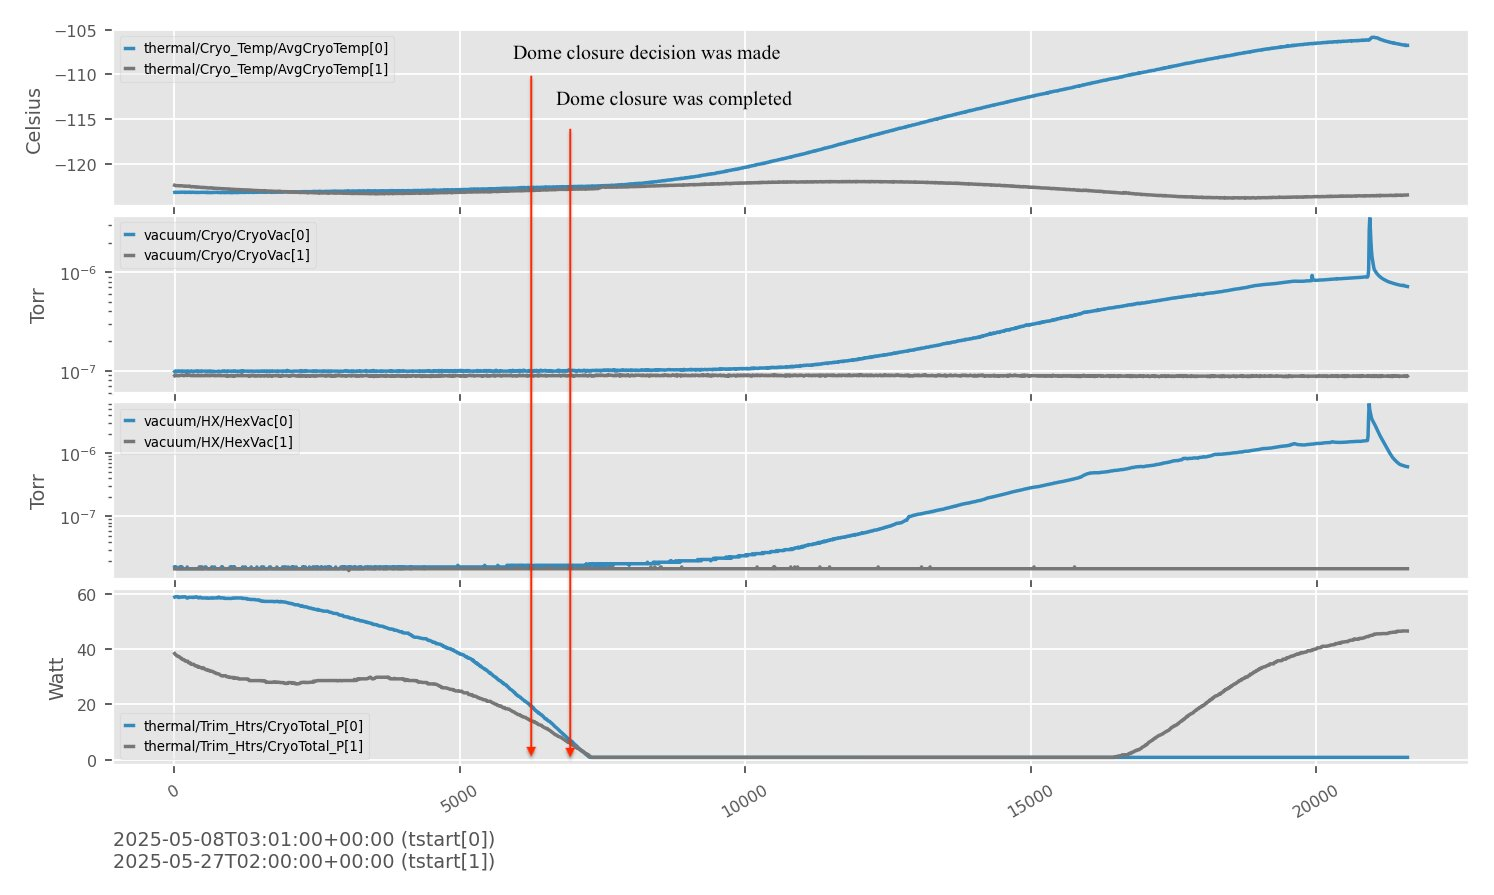
\includegraphics[width=0.60\textwidth]{issues2025/figs/CRYO-01-a.jpg}
\\[4pt]
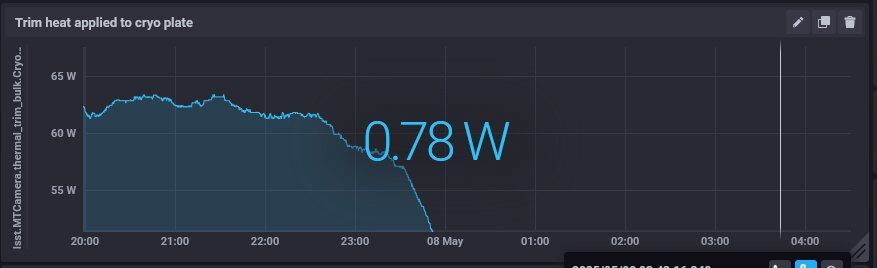
\includegraphics[width=0.90\textwidth]{issues2025/figs/CRYO-01-b.jpg}
\caption{\textbf{CRYO-01.} Top: the 8 May loss of capacity as it was reconstructed afterwards --- cryo temperatures, cryostat and heat-exchanger vacuum and the cryo-plate trim heat, with the moments the dome-closure decision was taken and completed marked (2025-05-27).  Bottom: trim heat applied to the cryo plate falling to 0.78\,W, the floor at which the plate can no longer be held in control (2025-05-25).}
\label{fig:iss-CRYO-01}
\end{figure}

\item[CRYO-02]\label{iss:CRYO-02} \textbf{Cryo 1 heat-exchanger return temperature below the dome dew point.}
  \emph{First to last mention 2025-05-12 to 2025-09-09; status \textcolor{stopn}{\textbf{Open}}.}
  Cryo~1's heat-exchanger return line ran colder than the in-dome dew point, risking frost or an ice sheet on the plumbing, and the circuit had to be stopped nightly for several weeks.  Throttling the liquid-line isolation valve (June~1--4) and then removing refrigerant to lower the discharge pressure raised the return temperature to about +3\,$^{\circ}$C, and in September the circuit was removed from the dome-closure decision criteria.  None of that was a fix: Cryo~1 recovered by itself, and the underlying question --- whether a low heat-exchanger return temperature at low refrigerant flow is acceptable --- has never been settled either way.  The clog now thought to lie behind it is registered as CRYO-04.  Experience since, including in high humidity, gives no indication that it is critical, but establishing that would require measuring the tube temperature against the temperature and humidity of the surrounding air.  Nothing further appears in 2026; the question of whether a low heat-exchanger return temperature at low refrigerant flow is acceptable was never taken up again. The trim-heat and dome-closure behavior that accompanies these nights is shown in Figure~\ref{fig:iss-CRYO-01}.

\item[CRYO-03]\label{iss:CRYO-03} \textbf{Cryo 6 compressor failure.}
  \emph{First to last mention 2025-04-01 to 2025-06-07; status \textcolor{stres}{\textbf{Resolved}}.}
  Cryo~6 tripped on a compressor failure on April~1 and stayed out of service.  The compressor module was replaced with the Cryo~5 unit from the MRCR between June~2 and June~7 (\lsstls{LCA-14623}), and after charging, gas chromatography and additive top-up the circuit returned to service, restoring six of six cryo circuits.

\item[CRYO-04]\label{iss:CRYO-04} \textbf{Suspected capillary clogs on Cryo 1, Cryo 3 and Cryo 4.}
  \emph{First to last mention 2025-05-12 to 2026-06-26; status \textcolor{stopn}{\textbf{Open}}.}
  Three circuits developed what was read as a restriction at the capillary: Cryo~1 from around May~10, Cryo~3 on the recharge that followed the nitrogen contamination of CRYO-06, and Cryo~4 in early December.  Power cycling did not clear any of them --- Cryo~1 was cycled of order 30--60 times --- and neither did adding refrigerant or running the telescope horizontal.  Two came back on their own: Cryo~4 overnight on December~10, Cryo~1 over some months, with no one intervention creditable.  Cryo~3 did not; it was given up on October~20 and the camera has run on five of six circuits since.  The low heat-exchanger return temperature Cryo~1 was left with is CRYO-02.  Two more circuits joined in 2026.  Cryo~2 clogged at C3 and was flushed in March, clogged again, refused to pass nitrogen at all in May --- ``absolutely zero flow'' --- and was set aside until an R123 flush in August.  Cryo~6 clogged at C4 and was cleared by the June purge.  Cryo~1 clogged again on its liquid line in May, and the replacement compressor fitted to Cryo~4 in June arrived with a C3 clog of its own.  Refrigerant was added repeatedly to buy margin.  Of the six circuits, two were out of service and one degraded when the record ends.

\begin{figure}[H]
\centering
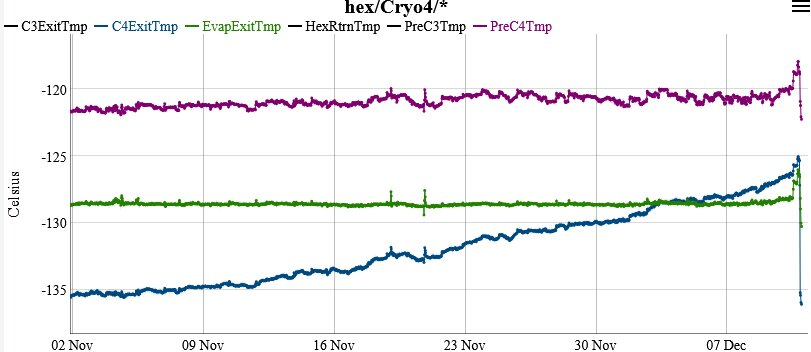
\includegraphics[width=0.90\textwidth]{issues2025/figs/CRYO-04-a.jpg}
\caption{\textbf{CRYO-04.} The Cryo~4 clog developing through November: the C4 exit temperature (blue) drifts up toward the pre-capillary temperature over 5 weeks, the signature by which the clog was recognized (2025-12-11, \#cam-operator).}
\label{fig:iss-CRYO-04}
\end{figure}

\item[CRYO-05]\label{iss:CRYO-05} \textbf{Cryo 6 PLC death after an external setpoint change.}
  \emph{First to last mention 2025-11-18 to 2026-06-24; status \textcolor{stopn}{\textbf{Open}}.}
  On November~19 the Cryo~6 PLC was declared dead at 00:34\,UTC with the discharge temperature reading 122\,$^{\circ}$C and the oil level negative; the PLC recovered by itself 33 minutes later.  The overheating of the cabinet that preceded it was attributed to a software update elsewhere on the summit mis-setting the glycol setpoint in response to bad environmental sensor readings (\rubintkt{FRACAS-322}, \rubintkt{OBS-1394}, \rubintkt{OBS-1395}).  The PLC failure itself is suspected to be a problem in the PLC, and its root cause is not known.  The CCS logic that closes the coolant valve when a PLC is declared dead was flagged as needing revision (\slactkt{LSSTCCSREFRIG-319} and \slactkt{LSSTCCSREFRIG-332}).  It happened three more times.  Cryo~6 dropped into a dead PLC state twice on 2026 May~8 (\rubintkt{LSSTCAM-174}, \rubintkt{LSSTCAM-175}) and again on June~24 --- the day after the controller had been swapped for the fault (\rubintkt{SUMMIT-12738}).  Moving the network switch port and power-cycling recovered it, and a suspect Ethernet cable was named but not replaced.  The root cause is still unknown.

\begin{figure}[H]
\centering
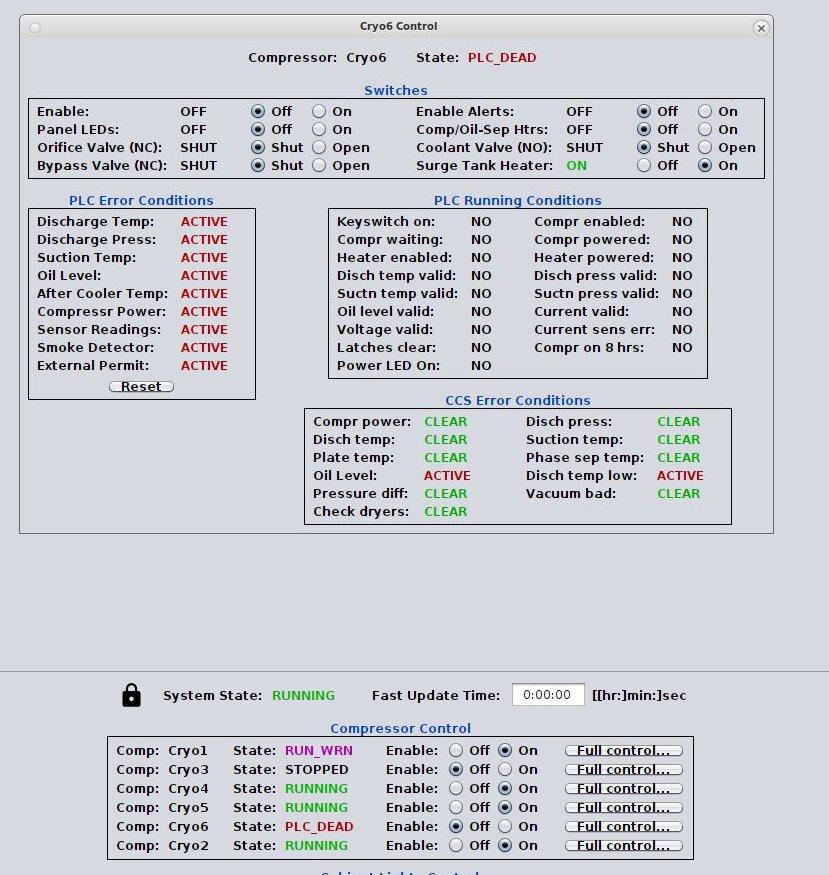
\includegraphics[height=6.20cm]{issues2025/figs/CRYO-05-a.jpg}\hfill
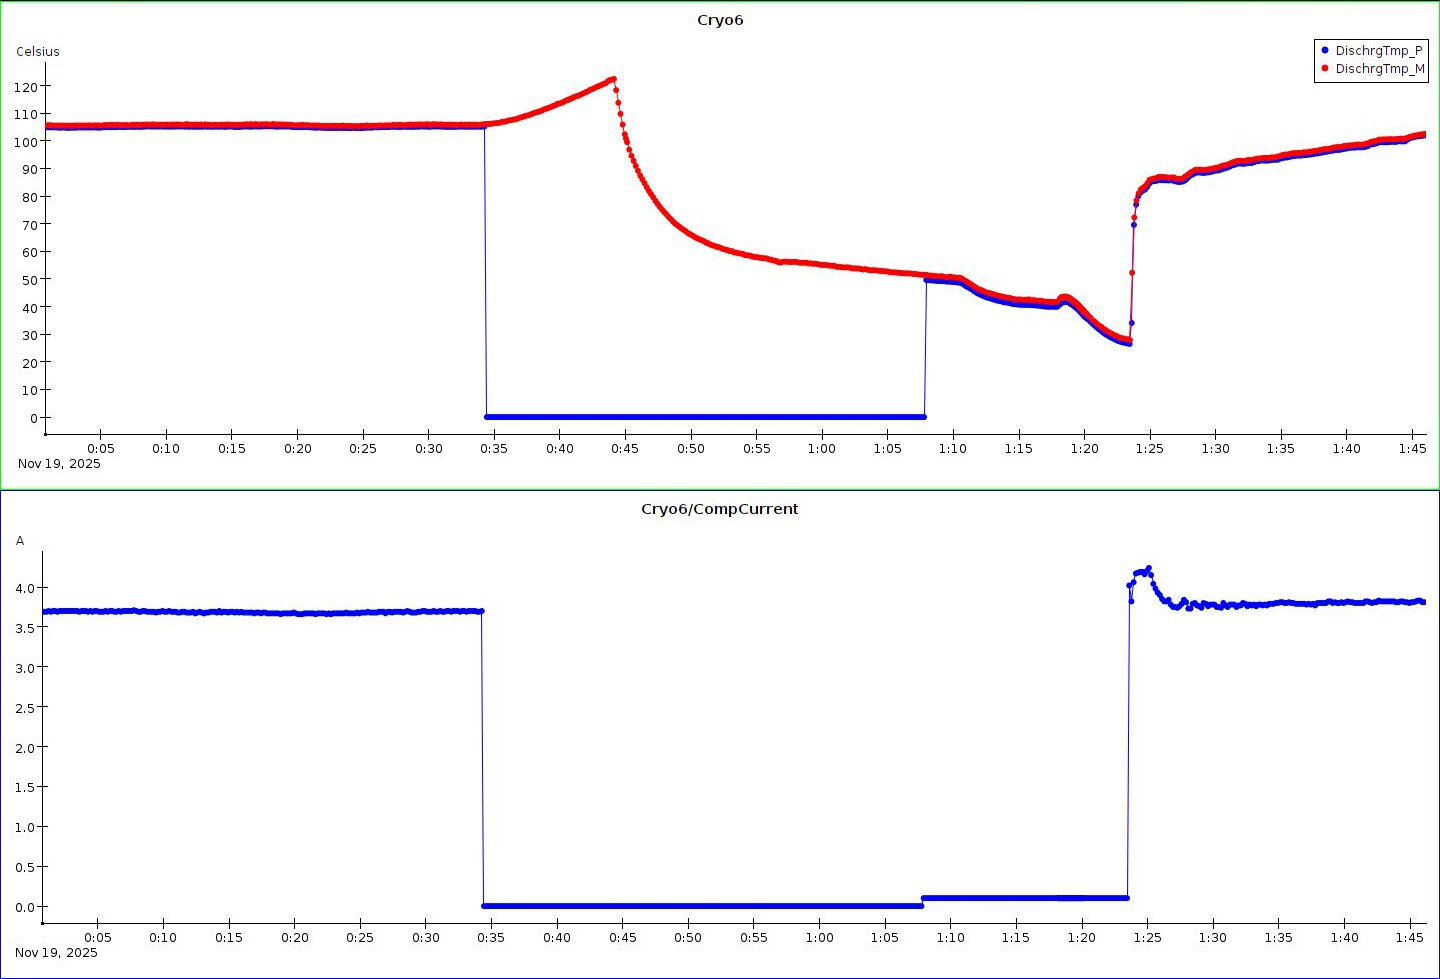
\includegraphics[height=6.20cm]{issues2025/figs/CRYO-05-b.jpg}
\caption{\textbf{CRYO-05.} Left: the CCS Cryo~6 panel during the failure, reporting \texttt{State: PLC\_DEAD} with every PLC error condition ACTIVE.  Right: the discharge temperature and compressor current across the event, the temperature rising while the compressor is off (2025-11-19).}
\label{fig:iss-CRYO-05}
\end{figure}

\item[CRYO-06]\label{iss:CRYO-06} \textbf{Nitrogen contamination of cryo circuits during maintenance.}
  \emph{First to last mention 2025-05-26 to 2025-10-16; status \textcolor{stmit}{\textbf{Mitigated}}\,\textbf{?}.}
  Twice in the year nitrogen got into a refrigeration circuit during work on it, by two different routes, and in both cases it was recognized only afterwards.  Cryo~2 took about 45\,grams during an oil addition on April~2; the resulting high discharge pressure was carried for months and was not explained until May~26, and the circuit was still sitting at 420\,psi discharge in mid-June with refrigerant removal under discussion as the remedy.  In October, during the filter-dryer replacement campaign, nitrogen reached the refrigerant in Cryo~3: the filter dryer was pressurized with nitrogen above the pressure of the rest of the circuit and a cross-leaking isolation valve --- described afterwards as stuck open --- let it through.  Cryo~3 had to be evacuated over the weekend of October~11--12 and recharged, and it is on that recharge that it developed the clog which cost it the rest of the year (CRYO-04).  The corrective action is procedural and was stated precisely on October~16: confirm the isolation valve is fully closed before pressurizing the filter dryer with nitrogen, and never pressurize the filter dryer above the pressure of the remaining circuit.  Revisions to \lsstls{LCA-14625} (evacuation and charging) and \lsstls{LCA-17726} (filter-dryer replacement) were promised for that week; whether they were issued is not visible in these channels.  A third suspicion --- that nitrogen entered Cryo~1 during a filter-dryer swap and explained its poor performance --- was raised on May~26 and ruled out on the physics: nitrogen raises the discharge pressure but cannot produce a low heat-exchanger return temperature.

\item[CRYO-07]\label{iss:CRYO-07} \textbf{Cryo 5 compressor failure and refrigerant-line leak.}
  \emph{First to last mention 2026-05-01 to 2026-07-13; status \textcolor{stopn}{\textbf{Open}}.}
  Cryo~5 tripped on 2026 May~1 at 19:49\,UTC on a 3886\,W power spike and its compressor was found burnt.  The spare compressor from Cryo~2 was fitted by May~13, but the circuit would not hold and was given up on May~16.  The reason emerged during the Cryo~4 emergency of late June: the circuit has an active refrigerant leak at a hose-barb crimp fitting.  A cut-and-reclamp repair on June~23 failed its hold test by a wide margin --- vapor pressure fell from 410.9 to 326.3\,psia in 22 minutes --- and the circuit was re-pressurized on July~9 without holding either.  An E-Z-Clip reassembly was being considered instead when the summit closed.  Cryo~5 has been out of service since May~1.

\item[CRYO-08]\label{iss:CRYO-08} \textbf{Cryo 4 compressor failure and the MRCR spare.}
  \emph{First to last mention 2026-06-20 to 2026-06-26; status \textcolor{stmit}{\textbf{Mitigated}}.}
  Cryo~4 failed overnight on 2026 June~20 with blown fuses, on the same signature as the Cryo~5 failure 7 weeks earlier, and the CCDs had to be turned off camera-wide.  The response was decided in an emergency meeting the next morning: fit the unmounted MRCR spare compressor rather than wait (\rubintkt{SUMMIT-12941}).  It was hoisted and installed on June~22, charged on June~23 and brought back on line.  Two defects came with it --- a capillary clog on C3, and glycol flowing the wrong way through the unit, found on June~26, whose correction cost about 10\,W of cooling capacity.  The camera has run on four of six circuits since.

\end{description}

\noindent\textit{Dynalene [utility-trunk cooling]}
\begin{description}
\item[DYN-01]\label{iss:DYN-01} \textbf{Recurrent loss of Dynalene flow to the utility trunk.}
  \emph{First to last mention 2025-01-18 to 2026-03-18; status \textcolor{stmit}{\textbf{Mitigated}}.}
  Dynalene, which cools the utility-trunk electronics, failed repeatedly all year --- from control computer (cRIO) reboots and crashes, chiller faults and power events --- each time forcing an emergency power-down of CCDs, REBs and often the shutter and filter changer (\rubintkt{OBS-1014}, \rubintkt{FRACAS-321}, \rubintkt{FRACAS-328}).  A review of the August~11 event established that the camera tolerates only about 13 minutes without flow before REB power-supply boards approach their 48\,$^{\circ}$C trip limit.  The cRIO was replaced on November~4 and a small UPS was added in late November, but outages continued into the second half of December.  January brought the worst of these events and then the fix.  On 2026 January~21 the cRIO failed, six or seven restart attempts failed with it, and the loss of flow ran long enough to put a utility-trunk sensor over its 35\,$^{\circ}$C limit --- ``A UT temperature went above the limit (35.0).  Turning off power.'' --- which shut the whole camera down (\rubintkt{OBS-1546}).  Recovery took until the 27th and included a physical cRIO swap and the disconnection of a faulty pressure-sensor bus.  A flow-regulator change on February~24 then raised the Level-6 manifold from 4.5 to 8\,bar and the camera flow from 5.2 to 7.6\,gpm, and it held through a real power outage 2 days later (\rubintkt{SUMMIT-12136}).  No loss of flow is recorded after March.

\begin{figure}[H]
\centering
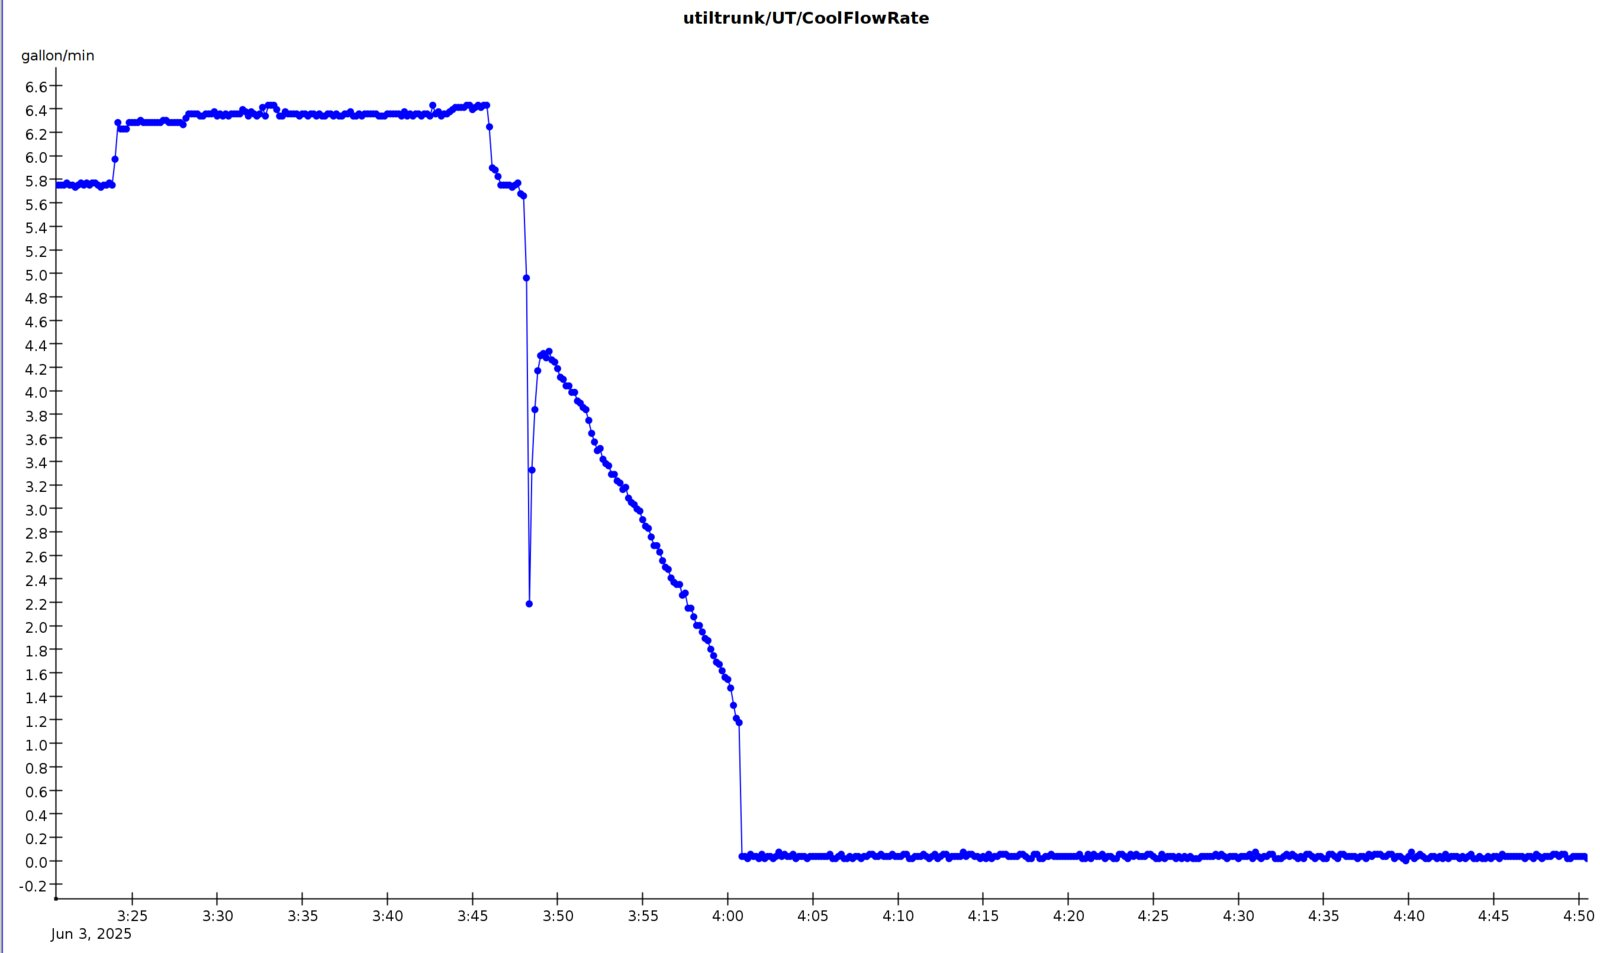
\includegraphics[width=0.62\textwidth]{issues2025/figs/DYN-01-a.jpg}
\caption{\textbf{DYN-01.} Utility-trunk Dynalene flow collapsing to zero.  This is the signature the events have in common: whatever the cause upstream --- a cRIO reboot, a chiller fault, a power event --- what the camera sees is the flow going away, and from that moment it has about 13 minutes before the REB power-supply boards approach their 48\,$^{\circ}$C trip limit (2025-06-03, \#cam-operator).}
\label{fig:iss-DYN-01}
\end{figure}

\item[DYN-02]\label{iss:DYN-02} \textbf{Camera warm-up on Dynalene chiller changeover and filter cleaning.}
  \emph{First to last mention 2025-02-21 to 2025-12-22; status \textcolor{stopn}{\textbf{Open}}.}
  Distinct from an outright loss of flow: routine facility actions --- weekly Dynalene filter cleaning, a clogged glycol filter, or switching between chillers --- warm the supply enough to push REB power-supply board temperatures toward their limit and trip the HV.  A clogged filter drove utility-trunk Dynalene to 22\,$^{\circ}$C in February, and on December~22 a chiller changeover forced HV and then the CCDs off for about an hour (\rubintkt{OBS-1490}).  No interlock or procedural gate prevents this at year end.  Nothing in 2026 beyond the weekly filter-cleaning reminders; no interlock was added. The flow signature is the one in Figure~\ref{fig:iss-DYN-01}; here it is the supply temperature rather than the flow that moves.

\item[DYN-04]\label{iss:DYN-04} \textbf{Condensation and humidity around the Top End Assembly.}
  \emph{First to last mention 2025-06-14 to 2026-02-28; status \textcolor{stopn}{\textbf{Open}}.}
  The camera region of the Top End Assembly runs more humid than ambient, and the compressed dry air supplied there has little authority over it --- the June investigation found the supply had been silently off for an unknown period and that the air reaching the camera is heavily mixed with dome air.  In November infrared imaging showed hot spots and a suspected dry-air leak near the heat-exchanger return, and in December water droplets were found on M1M3, traced to condensation on uninsulated Dynalene supply pipes at the Top End Assembly (\rubintkt{SUMMIT-11795}, \rubintkt{OBS-1479}).  Open at year end, with insulation the proposed fix.  Condensation during the January recovery was found ``everywhere in the observatory'', inside the PCS and cryo cabinets included, and a utility-trunk leak fault turned out to be condensation on the cable of the leak detector itself.  Dynalene setpoints were nudged twice in February against the dew point.  A purge-fan test at the end of February was inconclusive and the question was left as being broader than the fans.

\begin{figure}[H]
\centering
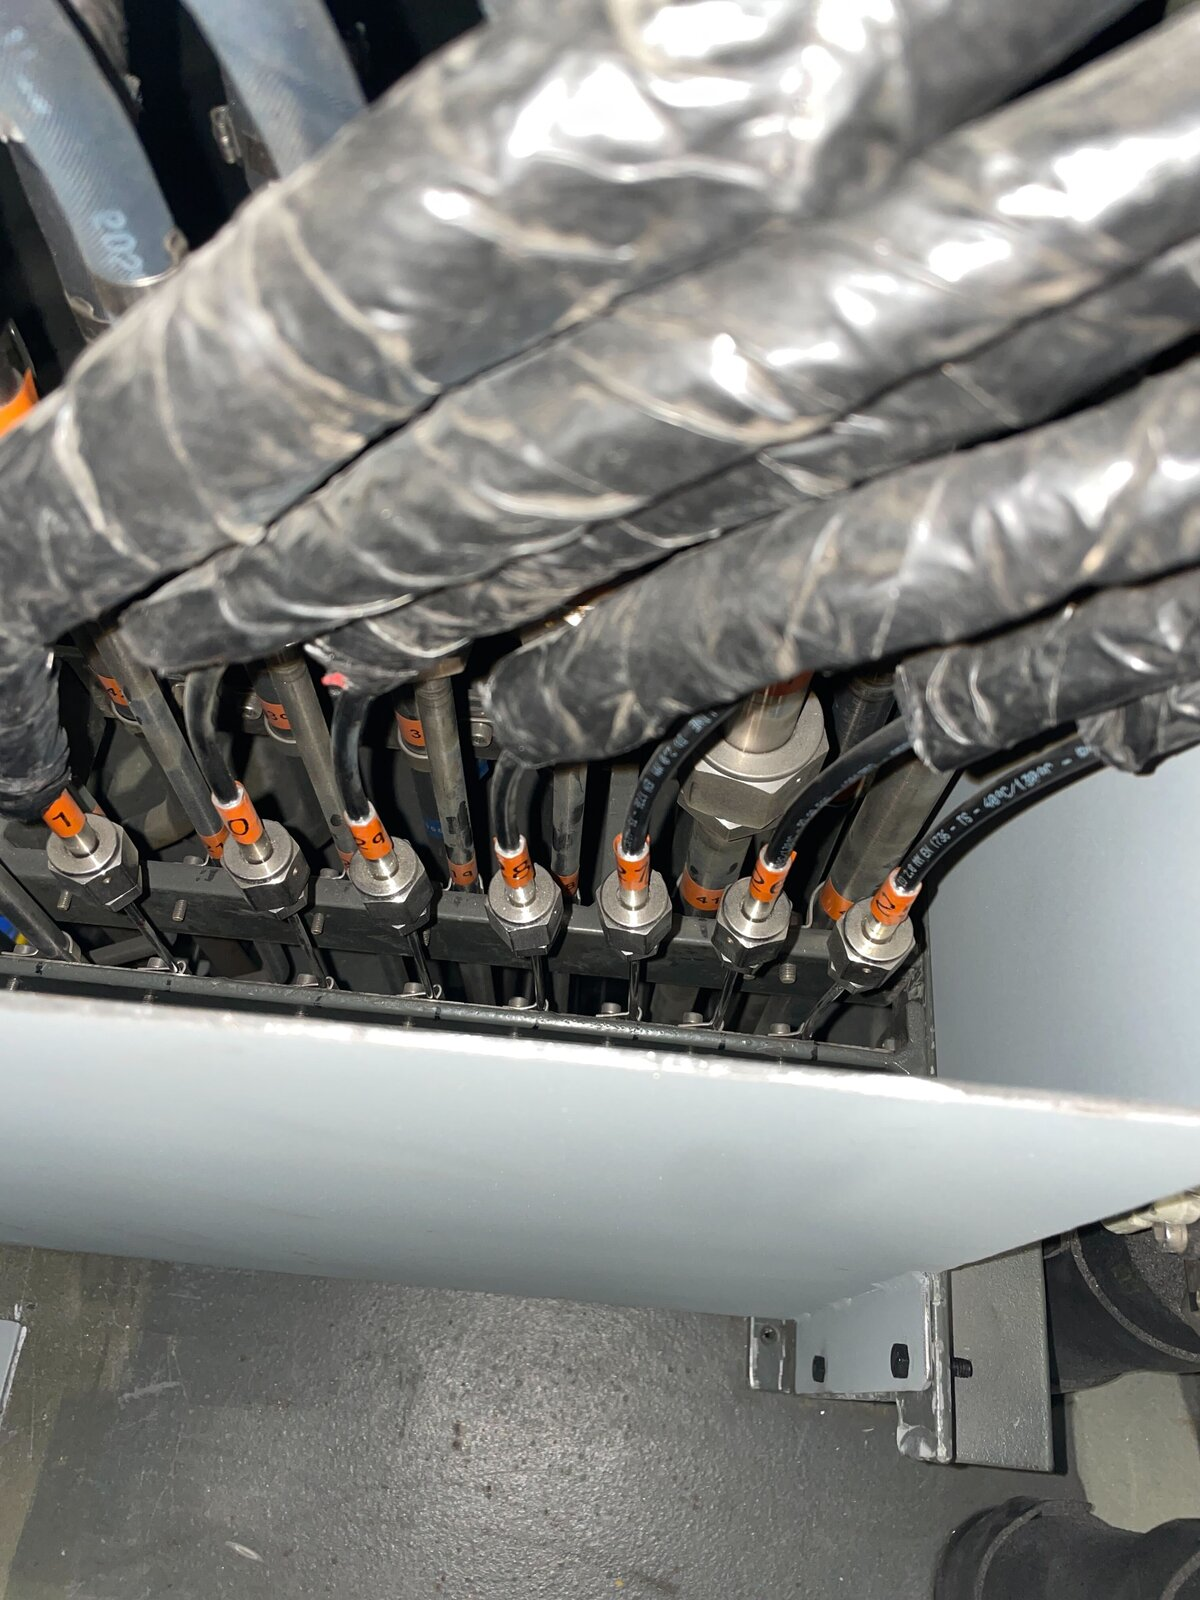
\includegraphics[height=6.50cm]{issues2025/figs/DYN-04-a.jpg}\hfill
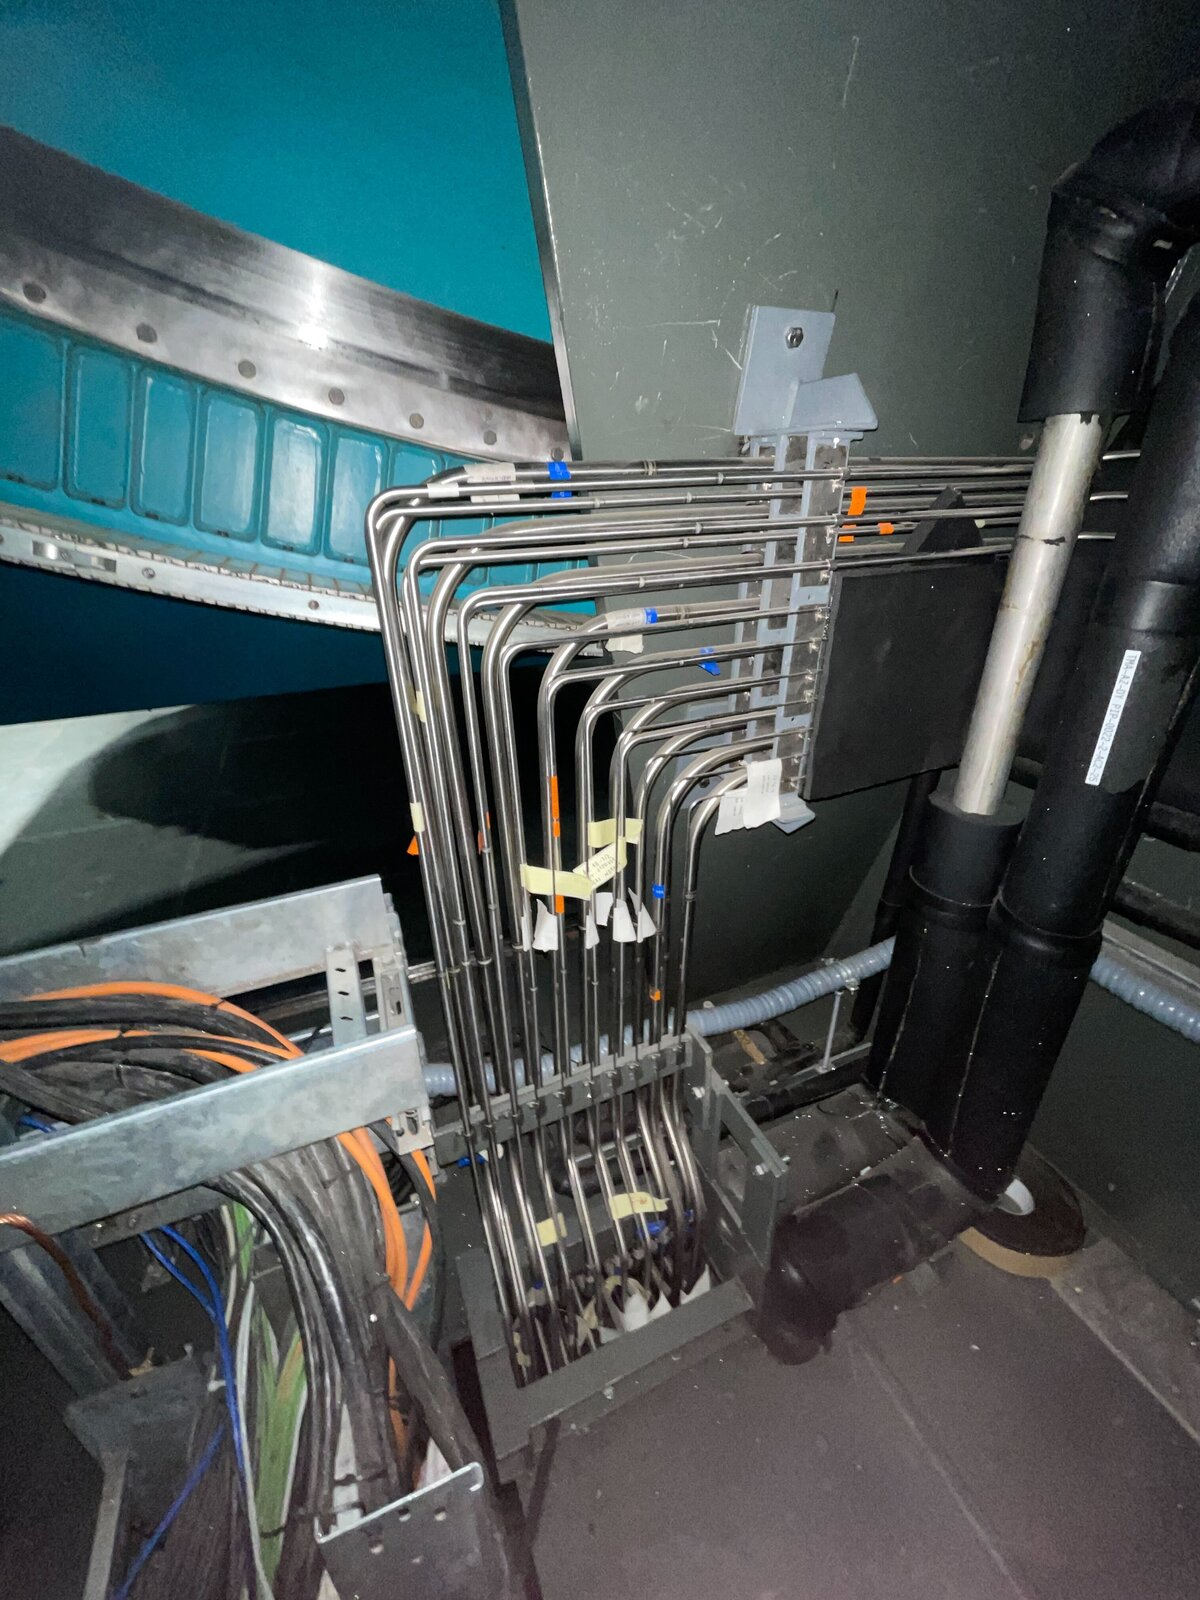
\includegraphics[height=6.50cm]{issues2025/figs/DYN-04-b.jpg}
\caption{\textbf{DYN-04.} Left: the liquid found below the camera cable wrap on 16~December, a little left of center looking into the mirror --- the drops that were traced back to the Top End Assembly.  Right: the source, measured a week later: an uninsulated Dynalene line at the cable wrap reading 1.6\,$^{\circ}$C on its surface, well below the dew point of the air around it (2025-12-16 and 2025-12-24, \#cam-summit-ops).}
\label{fig:iss-DYN-04}
\end{figure}

\item[DYN-05]\label{iss:DYN-05} \textbf{Age and handling of the Dynalene fluid.}
  \emph{First to last mention 2026-05-14 to 2026-05-19; status \textcolor{stopn}{\textbf{Open}}.}
  A large leak found near Level~7/8 on 2026 May~14 turned out to be the telescope's own circuit and not the camera's, but it opened a question that applies to both.  The Dynalene held at the summit has been stored in open containers for about 4.5 years against a manufacturer's specification of 5 years sealed, and a corroded copper joint was found during the investigation.  The camera's own plumbing contains copper --- the VPC and MPC heat exchangers and the brazed heat-exchanger pipe --- so the same corrosion mechanism applies to it.  Nothing was concluded.

\end{description}

\noindent\textit{Glycol [facility cooling]}
\begin{description}
\item[GLY-01]\label{iss:GLY-01} \textbf{Glycol flow interruptions to the PCS on power events.}
  \emph{First to last mention 2025-04-28 to 2026-07-13; status \textcolor{stmit}{\textbf{Mitigated}}.}
  Every commercial power glitch or generator transfer stops the glycol recirculation pumps for roughly 70--90 seconds, against an observed PCS chiller trip threshold of 90--120 seconds --- so each event is a near miss, and several were not (\rubintkt{FRACAS-277}, \rubintkt{FRACAS-278}, \rubintkt{FRACAS-279}).  The identified fix, putting the recirculating pumps on UPS, was still pending throughout 2025; in September, observing on generator power had to be restricted in pointing because of it.  The issue was closed in early February 2026, after the period covered here.  This is the entry that has to be taken back.  It was closed in early February 2026 --- and the flow had already been cut again on January~15 by a power glitch, ``something that should never happen as of mid December'' (\rubintkt{OBS-1525}), because the recirculating pump was never fully wired to ride one through.  The UPS-backed pumps were finished on February~19: ``Flow should never stop again for the known failure modes'' (\rubintkt{SUMMIT-12024}).  Flow stopped again on February~27, in March, in May, in June and 3 times in July.  The outages are now short --- tens of seconds rather than minutes --- so the fix did most of what was claimed for it, but the failure mode is not gone, and it has acquired a second form: a power cut leaves the site HVAC controller unable to restore its own setpoints (\rubintkt{FRACAS-402}).

\begin{figure}[H]
\centering
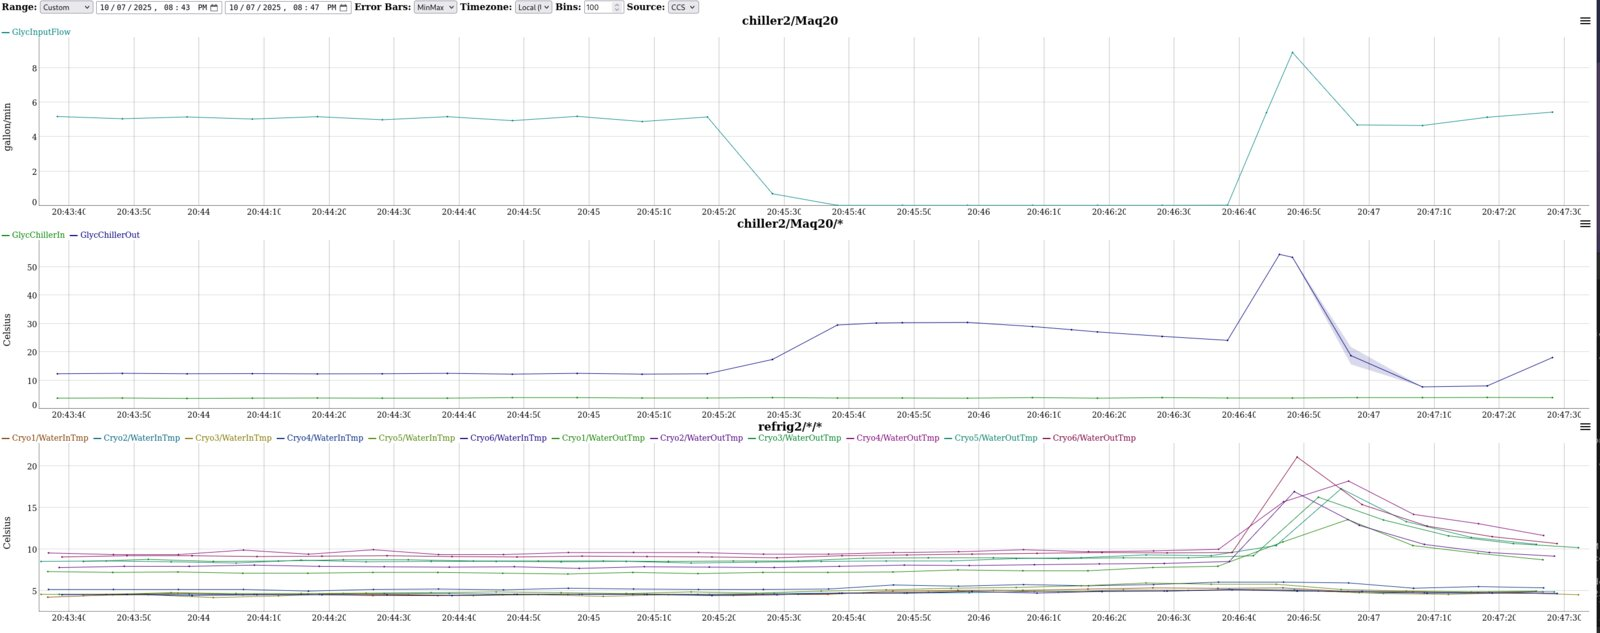
\includegraphics[width=0.90\textwidth]{issues2025/figs/GLY-01-a.jpg}
\caption{\textbf{GLY-01.} One of the near misses, at second resolution.  Glycol input flow to the PCS (top) drops from 5.2\,gallons per minute to zero at 20:45:30 and is restored about 70 seconds later; the chiller outlet temperature (middle) had already climbed from 12 to 30\,$^{\circ}$C before the interruption and overshoots to 54\,$^{\circ}$C on restart, and the cryo water-out temperatures (bottom) follow it up.  The chiller trips if the flow is lost for 90 to 120 seconds (2025-10-07, \#cam-operator).}
\label{fig:iss-GLY-01}
\end{figure}

\end{description}

\noindent\textit{Pumped-coolant system chiller}
\begin{description}
\item[PCS-01]\label{iss:PCS-01} \textbf{PCS chiller reliability.}
  \emph{First to last mention 2025-03-28 to 2026-04-30; status \textcolor{stopn}{\textbf{Open}}.}
  A cluster of PCS chiller problems in spring, all of them traced and fixed: an under-rated 32\,A supply breaker against a 50\,A service requirement, which tripped the chiller twice in one morning (\rubintkt{OBS-826}); a stage-1 refrigerant leak that took the chiller out of service for a day and left the camera quiescent overnight; and spurious trips with no real chiller anomaly, traced to an unseated pin in a refrigeration-permit connector on the telescope-side cabling and aggravated by TMA shaking tests (\rubintkt{SUMMIT-10642}, \rubintkt{SUMMIT-10652}).  The breaker was replaced, the leak repaired and the connector pins and shell renewed.  Reopened.  The PCS chiller failed overnight on 2026 March~19--20 on a compressor fault, and the REBs were off until the following afternoon.  The cause was a shorted cabinet fan, its thermostat set at 20\,$^{\circ}$C so that it ran continuously and reached the end of its one-year life, which tripped a breaker that also fed the compressor protection circuit.  The thermostat was lowered to 10\,$^{\circ}$C and spares were ordered (\rubintkt{SUMMIT-12289}).  The replacement fans delivered in April were found to contain the same material that had burnt.

\begin{figure}[H]
\centering
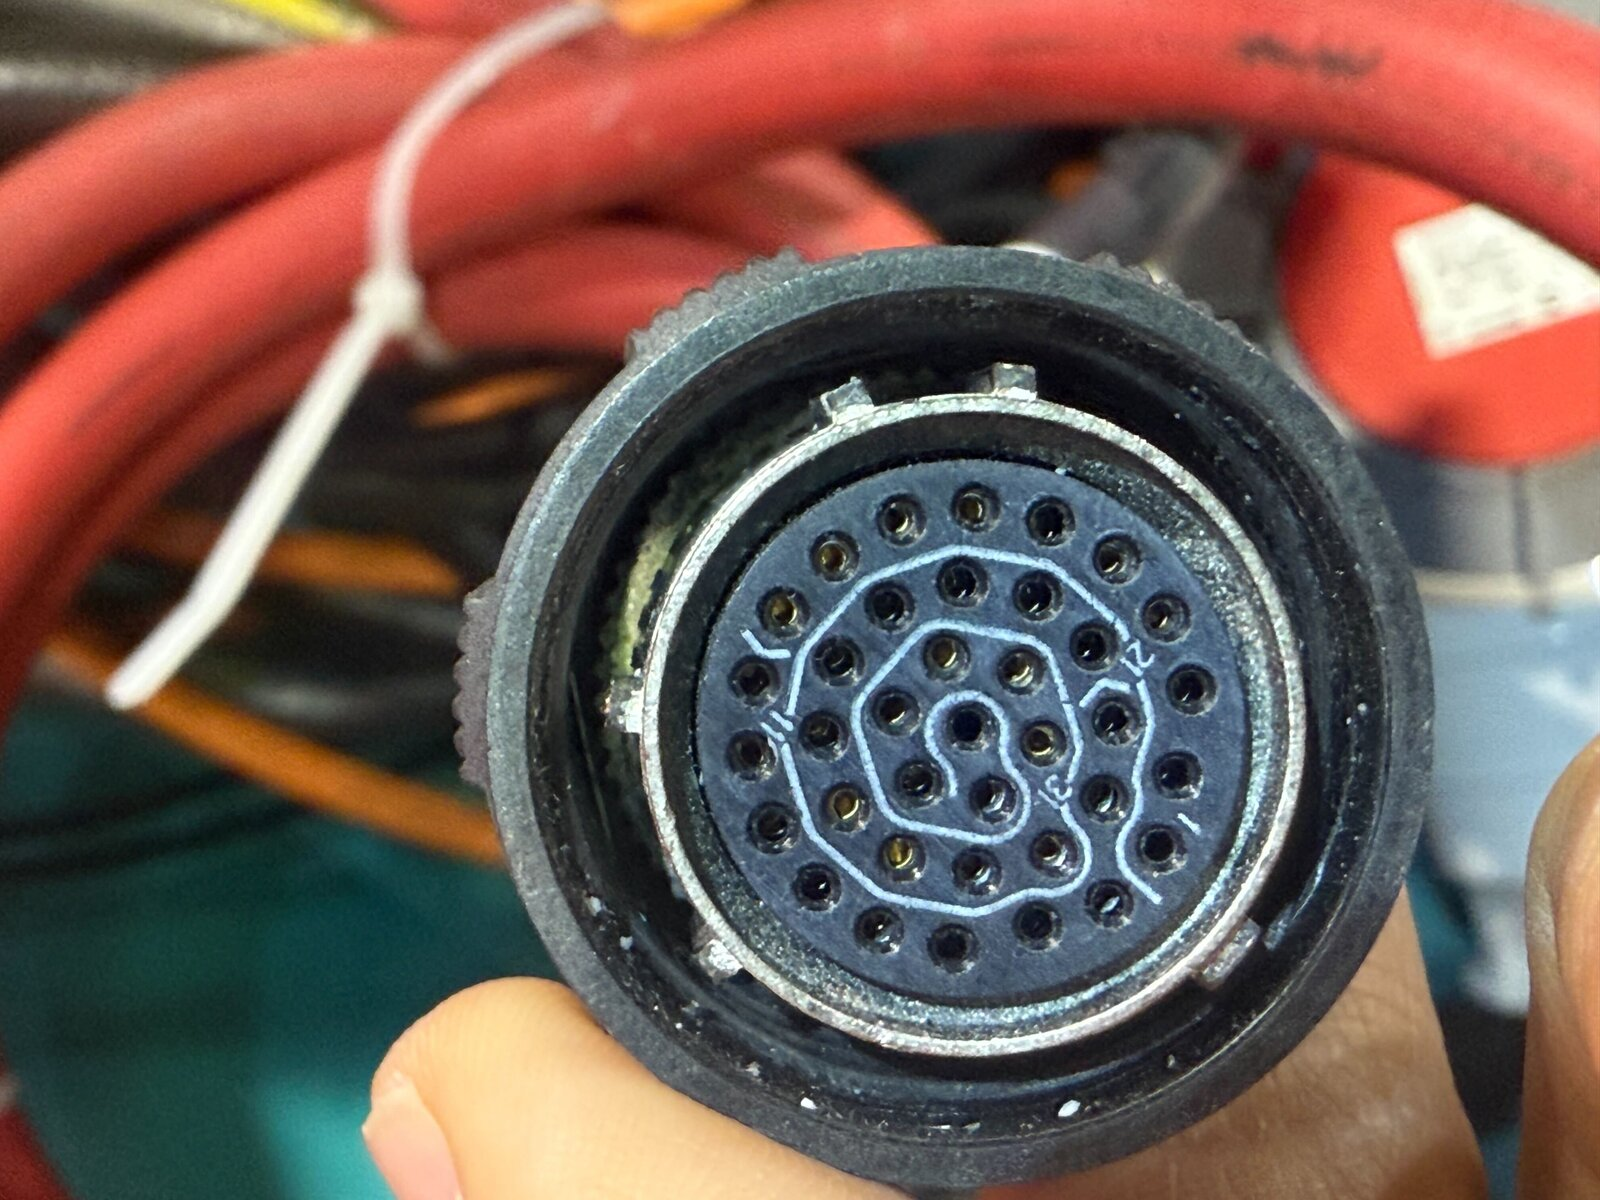
\includegraphics[width=0.62\textwidth]{issues2025/figs/PCS-01-a.jpg}
\caption{\textbf{PCS-01.} The pin face of the refrigeration-permit connector on the telescope-side cabling.  An unseated pin here is what produced the spurious chiller trips --- no chiller anomaly, a permit signal that came and went as the TMA moved.  The pins and the shell were renewed (2025-04-11, \#cam-operator).}
\label{fig:iss-PCS-01}
\end{figure}

\item[PCS-02]\label{iss:PCS-02} \textbf{PCS chiller restart difficulty, and the MRCR unit.}
  \emph{First to last mention 2025-03-28 to 2026-03-04; status \textcolor{stopn}{\textbf{Open}}.}
  Restarting the chiller is a separate problem from the failures above and was never solved: the unit repeatedly trips on low HFE flow because gas bubbles form in the longer line configuration, which procedure \lsstls{LCA-20281} does not cover.  In March it took roughly a dozen attempts over 2 days, and was recovered only by pressurizing the coolant tank; a loud bypass-valve noise during those attempts was later explained as the high-pressure bypass cracking at an 80\,psi pump differential.  The same behavior blocked the restart of the unit at the MRCR in July.  The MRCR system was found to have failed during the year and is tracked as \rubintkt{LSSTCAM-119}.  Two more awkward restarts, in January and March; the underlying difficulty is unchanged.

\begin{figure}[H]
\centering
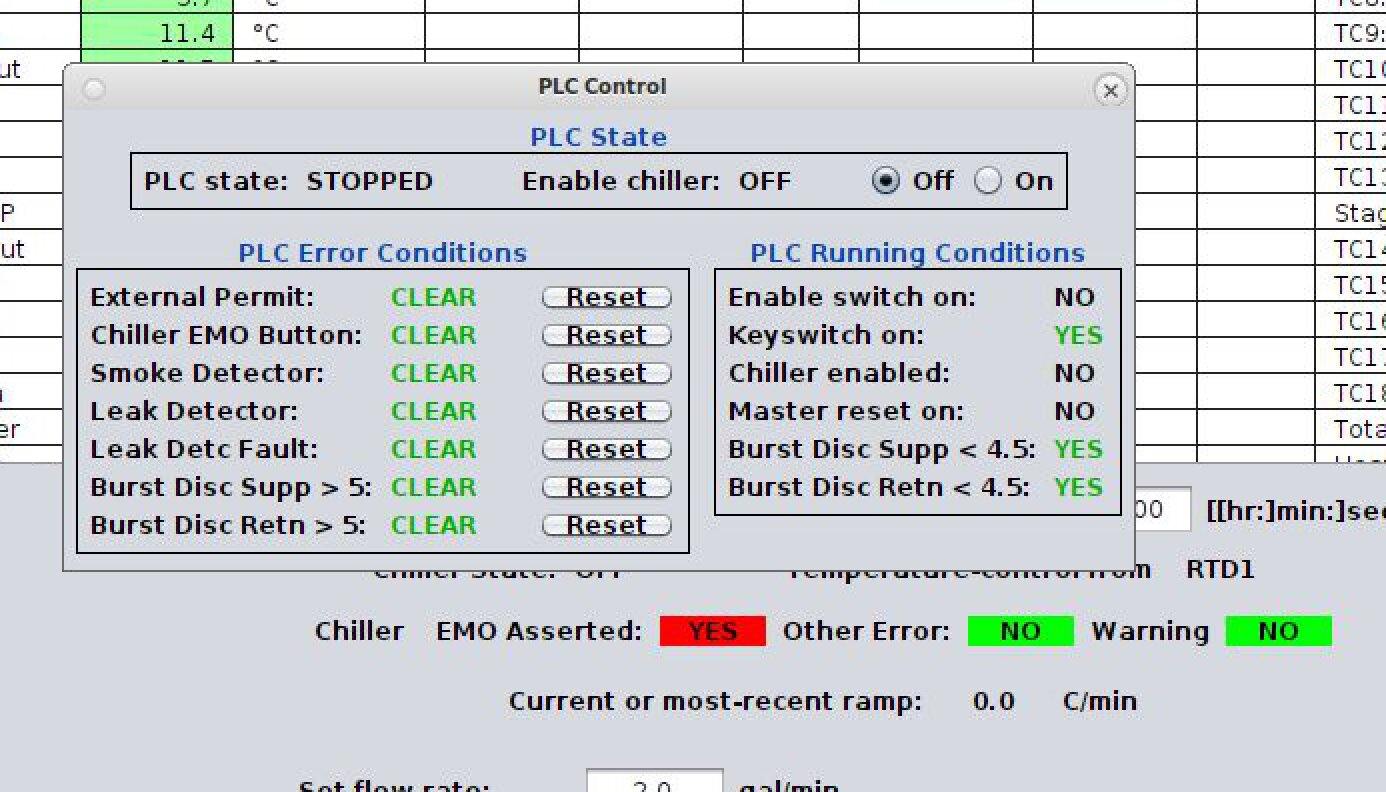
\includegraphics[width=0.62\textwidth]{issues2025/figs/PCS-02-a.jpg}
\caption{\textbf{PCS-02.} The chiller PLC panel during a restart attempt: stopped, with every error condition clear.  Nothing is reported as wrong, and the unit will still trip on low HFE flow when it is asked to start again --- which is why the restarts took about a dozen attempts over 2 days (2025-03-28, \#cam-operator).}
\label{fig:iss-PCS-02}
\end{figure}

\item[PCS-03]\label{iss:PCS-03} \textbf{Facility glycol capacity and the air handling units.}
  \emph{First to last mention 2026-03-06 to 2026-06-19; status \textcolor{stopn}{\textbf{Open}}.}
  The PCS chiller needs about 6.1\,gpm of glycol at 10\,$^{\circ}$C and degrades below 3--4.  Through 2026 it repeatedly did not get it.  Running all four site air handling units together pulls its flow down to about 2\,gpm and pushes its glycol-out temperature to 43--48\,$^{\circ}$C, so from March~6 the site ran three of four, toggled by observers at every dome opening (\rubintkt{SUMMIT-12191}).  A glycol chiller failure in April left the PCS on one chiller and ``redlining''; a bypass valve found open on April~21, wasting 600\,l/min of cold glycol, was worth 1.3\,gpm and 5--6\,$^{\circ}$C when closed.  In May a clogged PCS filter took the flow to 1.7\,gpm and forced the REBs off, and the recurring instability was traced to a chiller~2 setpoint its dirty evaporator could not reach (\rubintkt{FRACAS-387}).  The chiller-3 recirculation pump meant to settle it was still uncertified in mid-June.

\end{description}

\noindent\textit{Site power}
\begin{description}
\item[PWR-01]\label{iss:PWR-01} \textbf{Site power: grid glitches, generator failure and UPS capacity.}
  \emph{First to last mention 2025-02-25 to 2026-07-13; status \textcolor{stopn}{\textbf{Open}}.}
  The camera is exposed to the summit's power quality throughout: glitches stick valves closed (\rubintkt{FRACAS-282}), trip chillers and compressors, and interrupt cooling.  The most severe event was August~30, when the generator tripped --- its air inlet blocked by ice and snow (\rubintkt{FRACAS-299}) --- and left the camera on UPS alone.  The damage was not done by the loss of power to the camera itself but through the cooling chain: the glycol feeding the cryo circuits stopped with the recirculation pumps (GLY-01), the cryo systems were lost, and with them the cryostat pressure began to rise toward the ion-pump shutdown limit, at one point estimated to be about 15 minutes away.  The REBs and REB power supplies were shut down by hand while this was happening; generator power returned first and the pressure recovered.  Separately the server-room UPS exhausted its roughly 30-minute battery (\rubintkt{FRACAS-300}) and the backup diesel generator was found already out of service.  UPS batteries were replaced in November; the underlying exposure remains.  Glitches continued at much the same rate through 2026 and the camera absorbed them better than it had, thanks to the Dynalene and glycol work.  What they still do is upset the things downstream of them: the site HVAC controller loses its setpoints, a glycol chiller fails to restart, an air compressor stops.  Three power cuts in 1 day on July~3, and more on the 12th and 13th, were the last ordinary operating events before the summit closed.

\begin{figure}[H]
\centering
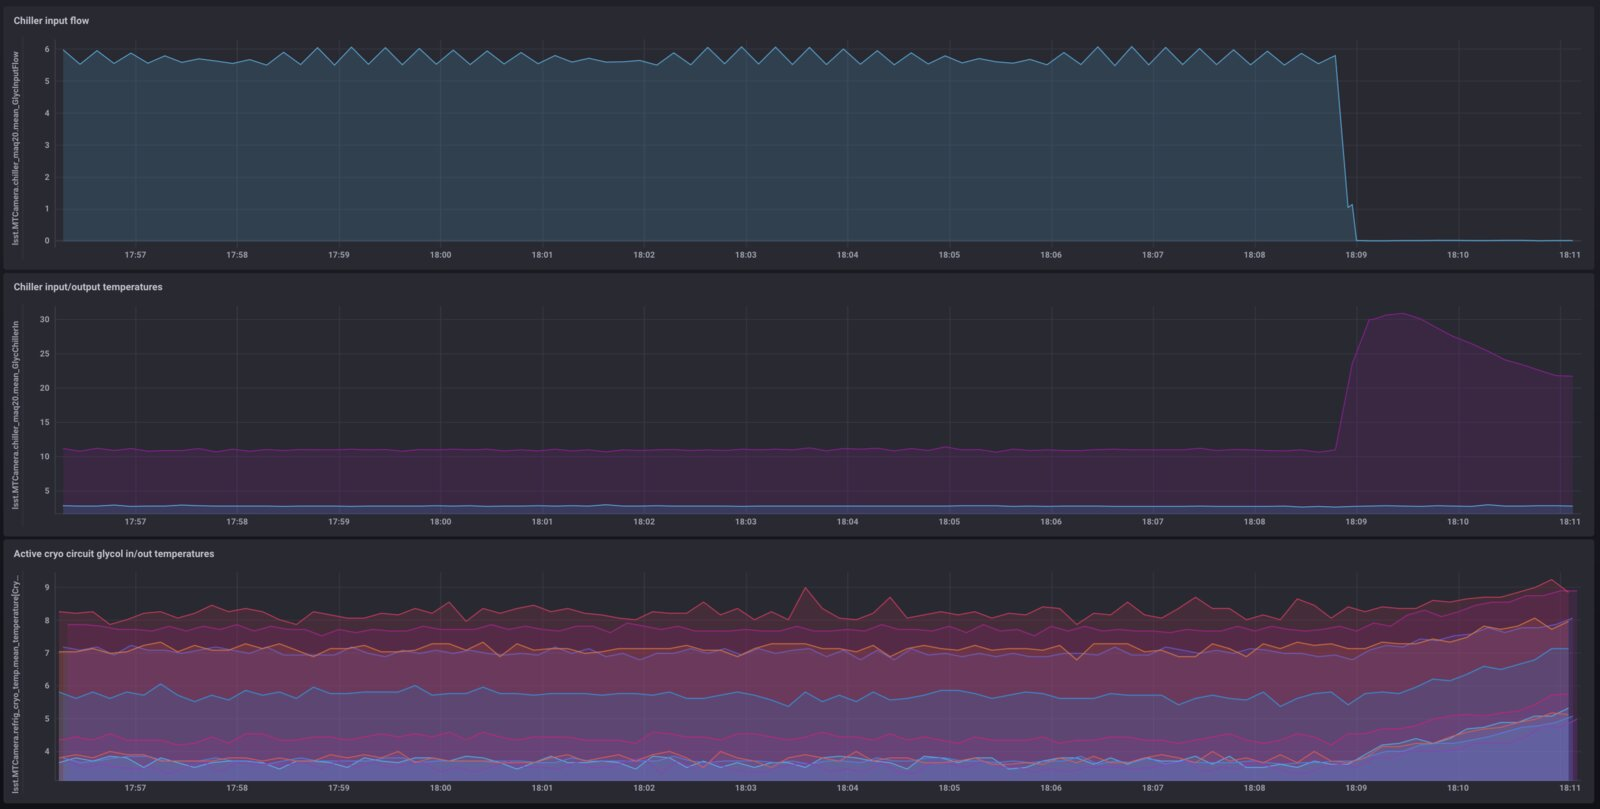
\includegraphics[width=0.60\textwidth]{issues2025/figs/PWR-01-b.jpg}
\\[4pt]
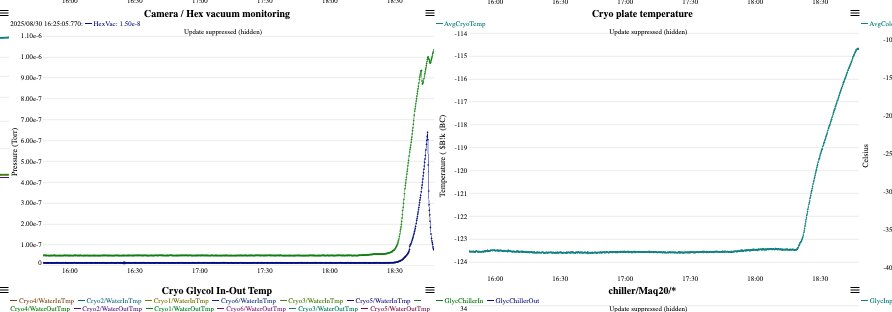
\includegraphics[width=0.90\textwidth]{issues2025/figs/PWR-01-a.jpg}
\caption{\textbf{PWR-01.} The chain of 30 August, in the order it happened.  Top: glycol input flow to the chiller collapsing when the generator trips, and the chiller outlet temperature stepping up as it goes --- ``No glycol flow to chiller.  Tripped.''  The cryo circuits go with it.  Bottom: the consequence some 20 minutes later --- cryostat and heat-exchanger pressure leaving $10^{-7}$\,Torr and rising past $1.1\times10^{-6}$, with the cryo plate warming from $-$124 toward $-$113\,$^{\circ}$C at about 0.6\,$^{\circ}$C per minute.  The ion-pump shutdown limit was estimated to be 15 minutes away when generator power came back (2025-08-30).}
\label{fig:iss-PWR-01}
\end{figure}

\item[PWR-02]\label{iss:PWR-02} \textbf{Mass REB power-supply trip of 7 July.}
  \emph{First to last mention 2026-07-07 to 2026-07-09; status \textcolor{stopn}{\textbf{Open}}\,\textbf{?}.}
  At 13:56:37\,UTC on 2026 July~7, 67 of 71 REBs tripped off at once.  Every REB power-supply board logged a voltage or current fault at essentially the same instant, across four separate 48\,V supplies, with the HV bias already off.  Inspection the next day found nothing, a single-REB test passed, and the camera was fully back by July~9.  No cause was established: ``We do not have firm evidence of a particular cause.  The consensus is a ground bounce event that was sufficient to trigger the RebPS safety system'' (\rubintkt{FRACAS-404}).  A coincident PDU alert was examined and rejected, since it could only have affected a sixth of the REBs.  Whether the open side panel and the vacuum work raised the electrostatic risk was asked and not answered.

\end{description}

\noindent\textit{Compressed dry air}
\begin{description}
\item[AIR-01]\label{iss:AIR-01} \textbf{Compressed dry air supply failures.}
  \emph{First to last mention 2025-02-27 to 2026-06-18; status \textcolor{stmit}{\textbf{Mitigated}}.}
  Compressed dry air operates the vacuum gate valves and purges the camera body, so its loss is a direct camera concern --- including frosting risk on the L3 lens.  Supply was cut for 2 hours for compressor maintenance in February, both Level-1 compressors degraded in August when their dryers froze at $-$8\,$^{\circ}$C, and a compressor was lost to a packing-seal failure in October.  Insulating jackets on the dryers addressed the freezing mode; single-compressor operation remains a routine condition.  The compressors faulted again in May (\rubintkt{FRACAS-385}) and once overnight in June, needing a remote restart; the operating procedure was rewritten afterwards to separate the manual and remote restart paths clearly.

\begin{figure}[H]
\centering
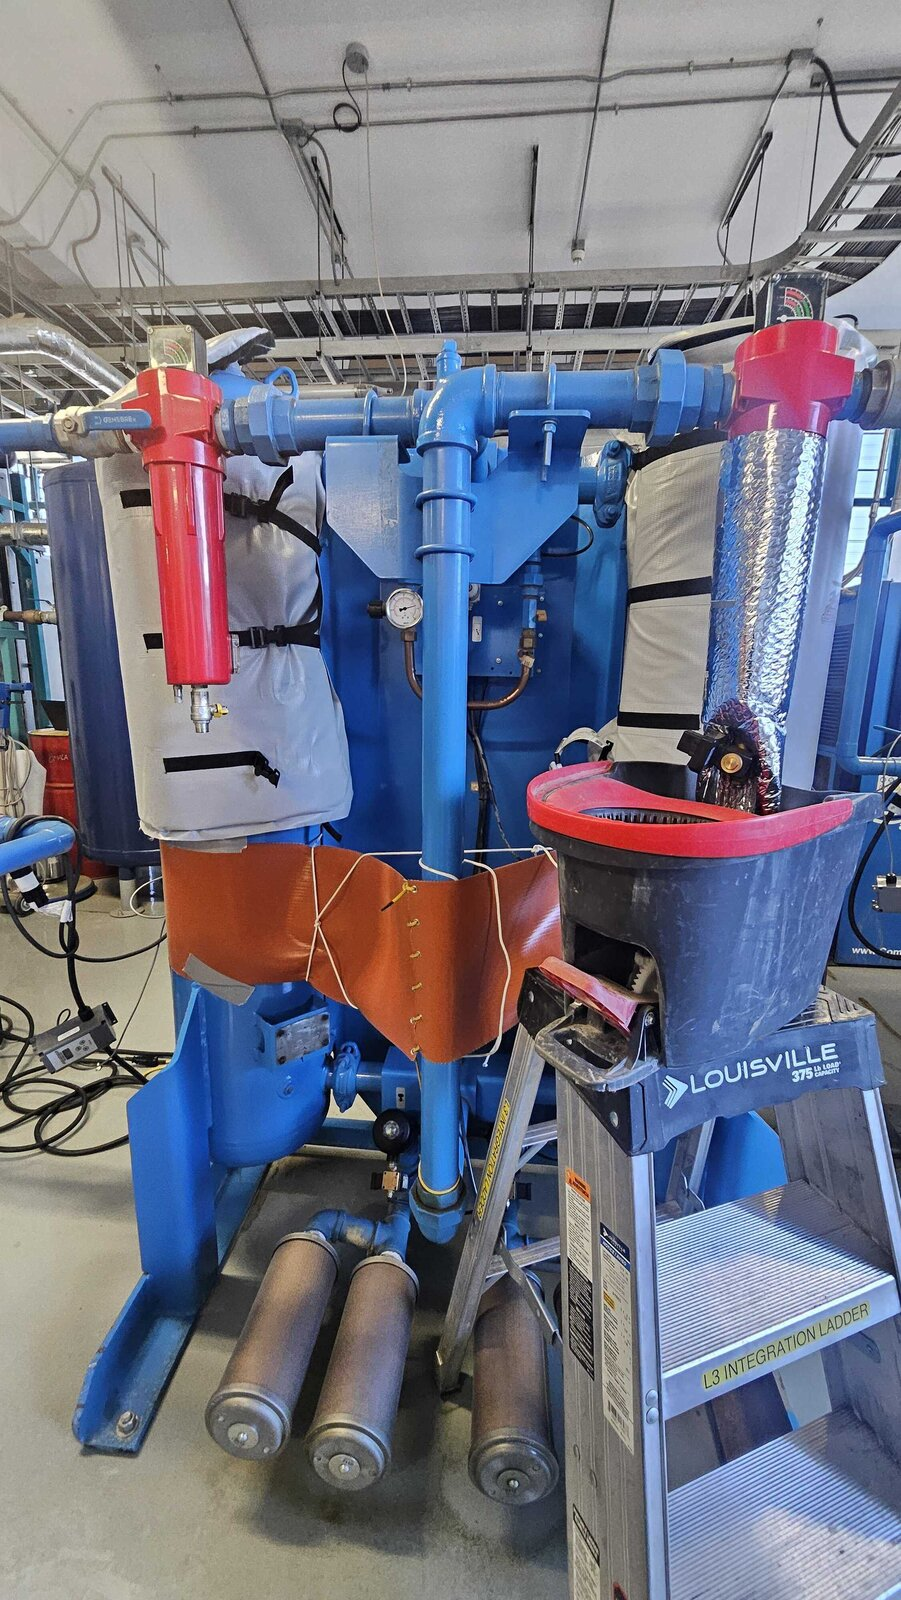
\includegraphics[height=6.50cm]{issues2025/figs/AIR-01-a.jpg}\hfill
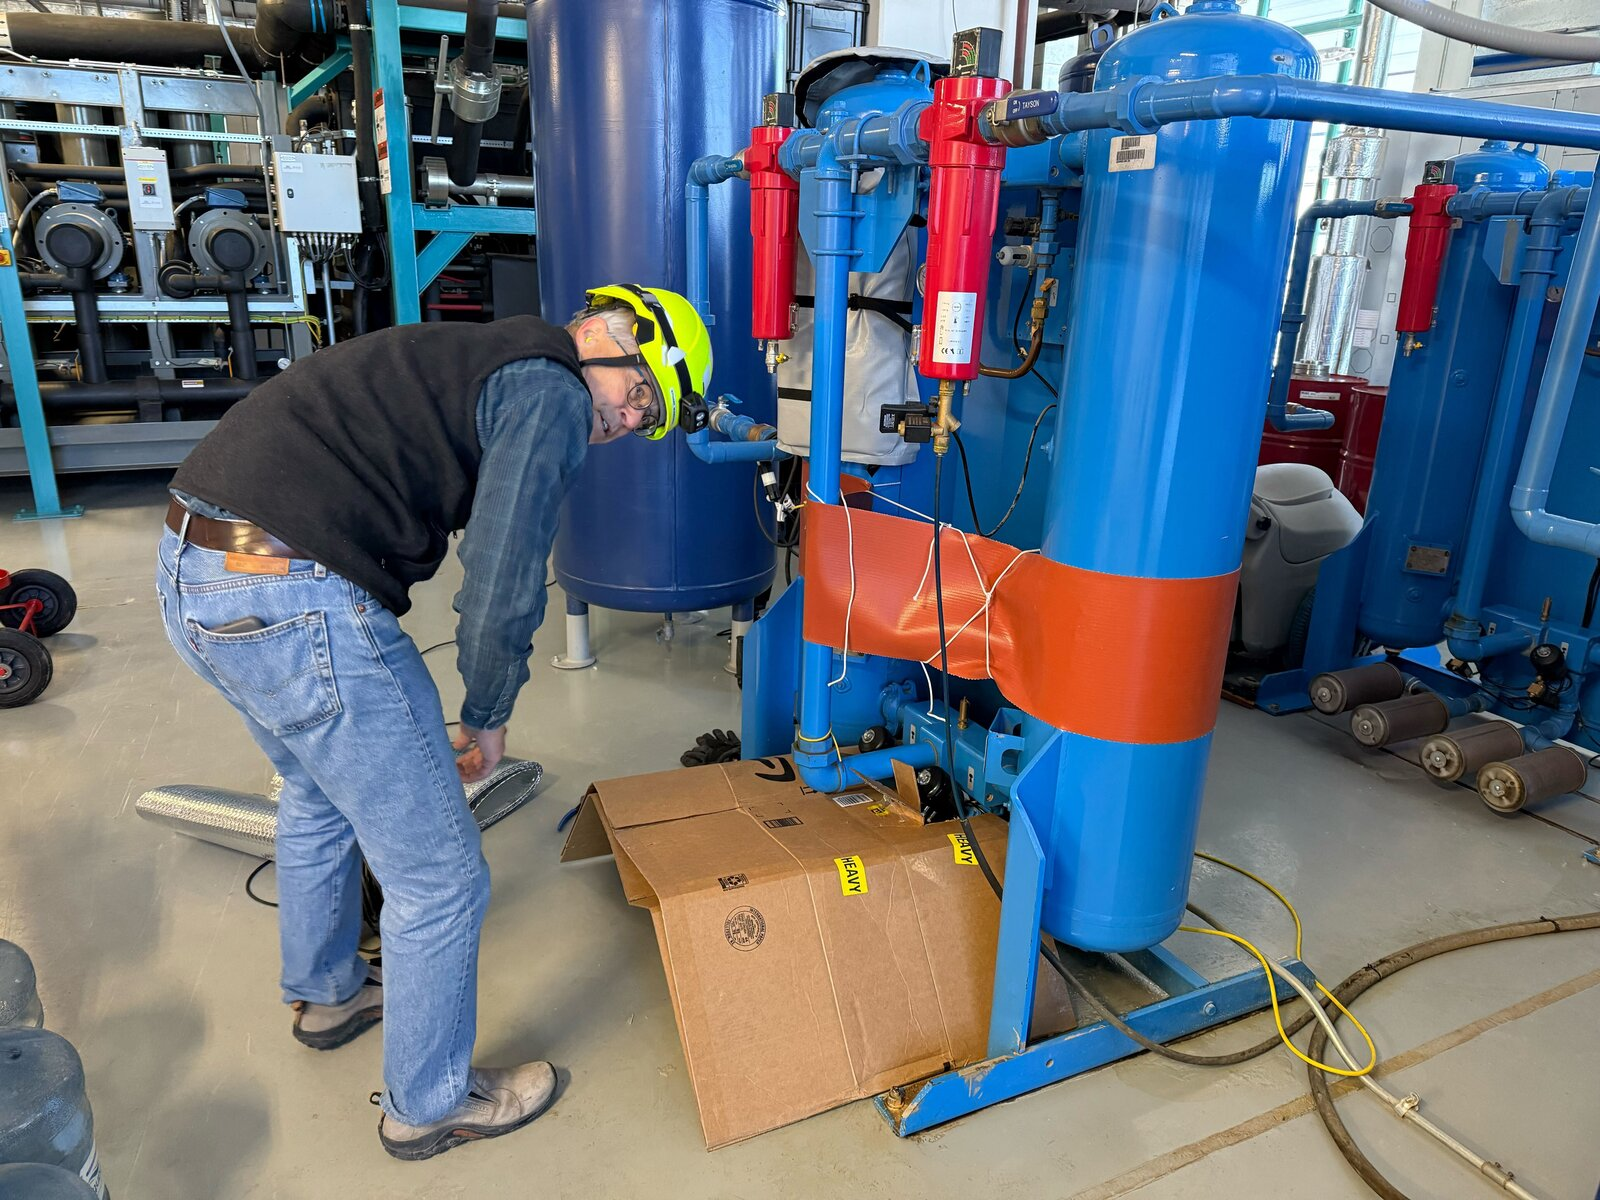
\includegraphics[height=6.50cm]{issues2025/figs/AIR-01-b.jpg}
\caption{\textbf{AIR-01.} The compressed-air dryers at Level~1, whose freezing in August stopped the air: the towers with their exhaust and drain lines, and the insulating jacket being fitted (2025-08-23 and 2025-08-26).}
\label{fig:iss-AIR-01}
\end{figure}

\end{description}

\noindent\textit{Focal plane}
\begin{description}
\item[FP-01]\label{iss:FP-01} \textbf{R30/Reb1/S12 suspected OD short (subject of this note).}
  \emph{First to last mention 2025-04-07 to 2025-12-10; status \textcolor{stwrk}{\textbf{Workaround}}.}
  On April~7, after a routine power cycle and a reorientation of the camera to zenith, R30/Reb1 raised a Bias2 OD2 overcurrent on S12 ($\mathrm{ODI}=0.213$\,A against an $0.082$\,A limit); S12 reached bias voltage in two steps and tripped off on both attempts, and the behavior was read at the time as a real short.  A retest on April~25 showed an unexplained digital-current spike of order 1\,A, and the REB was left as the only one switched off camera-wide through May.  It was returned to service on June~25--26 running two of three CCDs, which required an R30/Reb1 firmware update and relaxed bias-control limits; the CCD current on S12/Seg17 was noted as anomalously low at that turn-on and again on June~29.  The REB has carried its own firmware variant through every subsequent firmware campaign.  The workaround --- running two of the three CCDs on Reb1 --- was implemented on June~25--26 and has been in place since; the fault itself is unresolved. Described in detail in Sections~\ref{sec:r30s12} and~\ref{sec:r30s12-solution}.

\item[FP-02]\label{iss:FP-02} \textbf{R20/Reb2/S21 unphysical RD voltage read-back.}
  \emph{First to last mention 2025-04-02 to 2025-04-24; status \textcolor{stwrk}{\textbf{Workaround}}.}
  The April~2 CCD shorts test found R20/Reb2/S21 reading an unphysical $+54$\,V RD (reset drain) voltage; power cycling the REB and resetting the RCE did not change it, and the working theory was an open ADC input on the board.  The sensor blocked power-on of the raft until April~24, when the erroneous RD reading was configured to be ignored in software and R20 was returned to service.  No hardware repair was attempted. Described in detail in Section~\ref{sec:r20reb2}.

\item[FP-03]\label{iss:FP-03} \textbf{Non-linear HV bias behavior on R21/Reb0 and R12/Reb0.}
  \emph{First to last mention 2025-05-05 to 2026-07-09; status \textcolor{stwrk}{\textbf{Workaround}}.}
  R21/Reb0 repeatedly glitched and tripped its HV bias near 50\,V, where its DC-DC converter behaves non-linearly, once producing visible tree rings mid-integration.  It was set to run permanently at 46\,V, and R12/Reb0 later showed similar sensitivity requiring extra care during ramp-up.  Managed by lowered setpoints and careful ramping rather than repaired.  R21/Reb0 went on tripping on the ramp through 2026 and picked up two more workarounds: a hard DAC cap of 2582, and a faster idle clear during the ramp.  A periodic variation of the DAC on roughly a 77-minute cycle was noticed in May and not explained.  R12/Reb0 behaves the same way.

\begin{figure}[H]
\centering
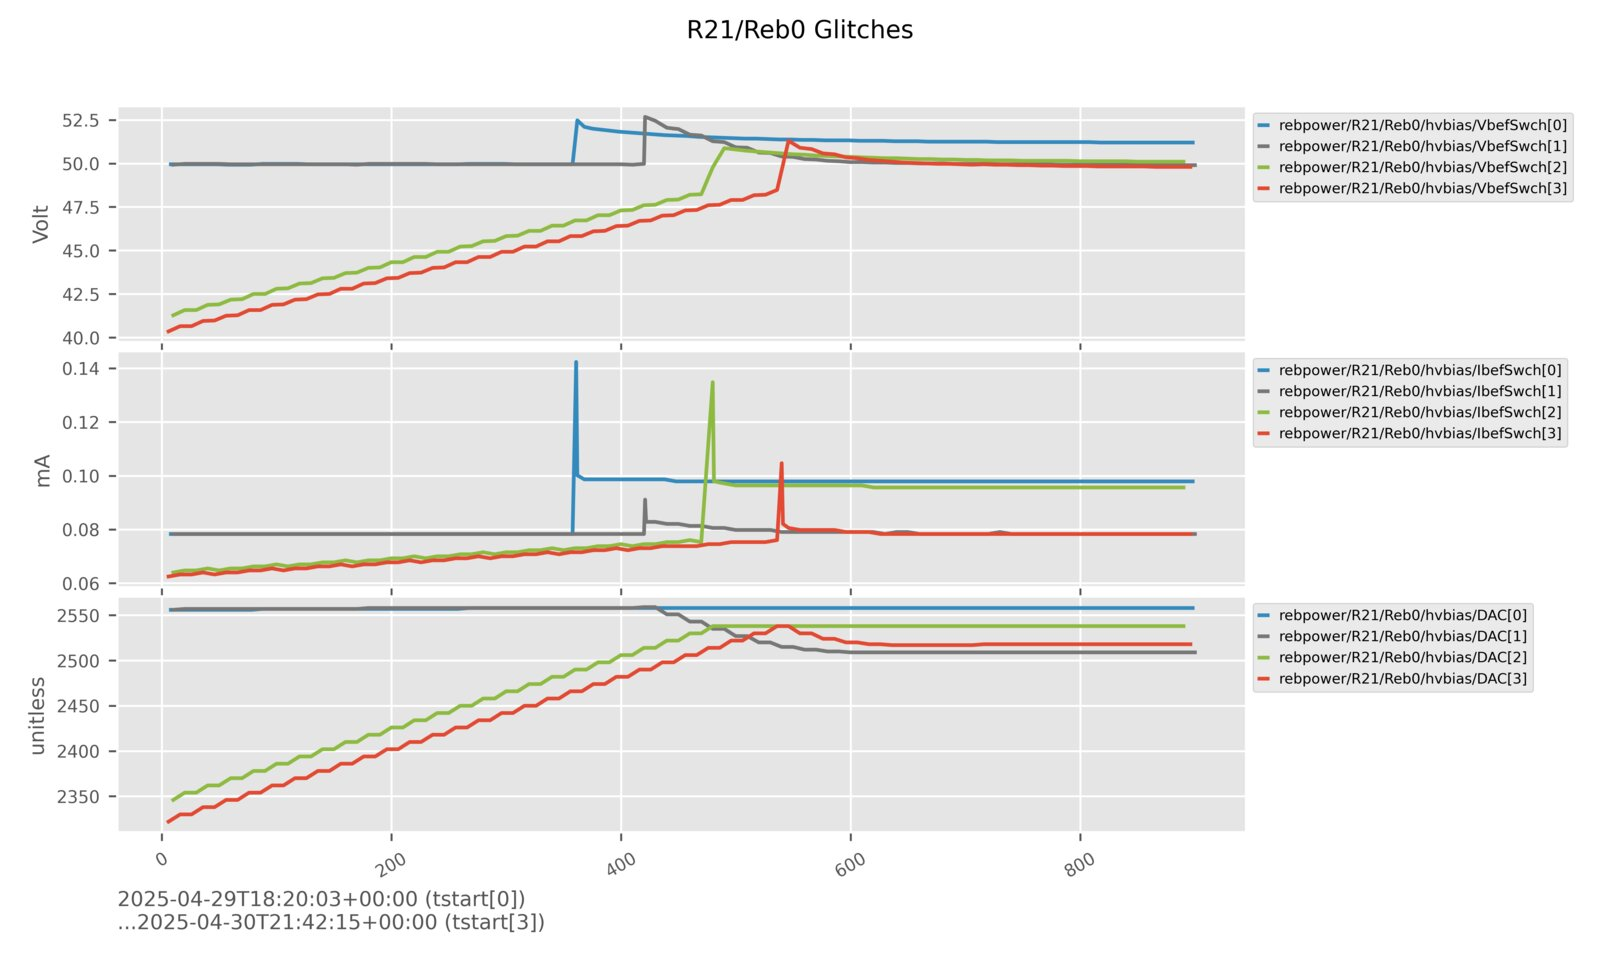
\includegraphics[width=0.62\textwidth]{issues2025/figs/FP-03-a.jpg}
\caption{\textbf{FP-03.} The glitches on R21/Reb0: HV bias voltage, current and DAC setting stepping and spiking as the bias is ramped, the behavior for which the operating point was lowered (2025-05-05, \#cam-operator).}
\label{fig:iss-FP-03}
\end{figure}

\item[FP-04]\label{iss:FP-04} \textbf{R03/Reb1/S11/Seg00 chronic bad amplifier.}
  \emph{First to last mention 2025-04-06 to 2025-05-10; status \textcolor{stwrk}{\textbf{Workaround}}.}
  A long-standing bad channel described in the logs as having gone ``back and forth from working to not, over the last few years''.  Its current stayed pinned at 0.5\,mA through repeated power cycles in April and May, and the neighbouring Amp16 also failed to return once.  The channel cannot be repaired in place; since the impact of a single amplifier is small, the decision is not to repair it and to continue operating with it as it is.

\begin{figure}[H]
\centering
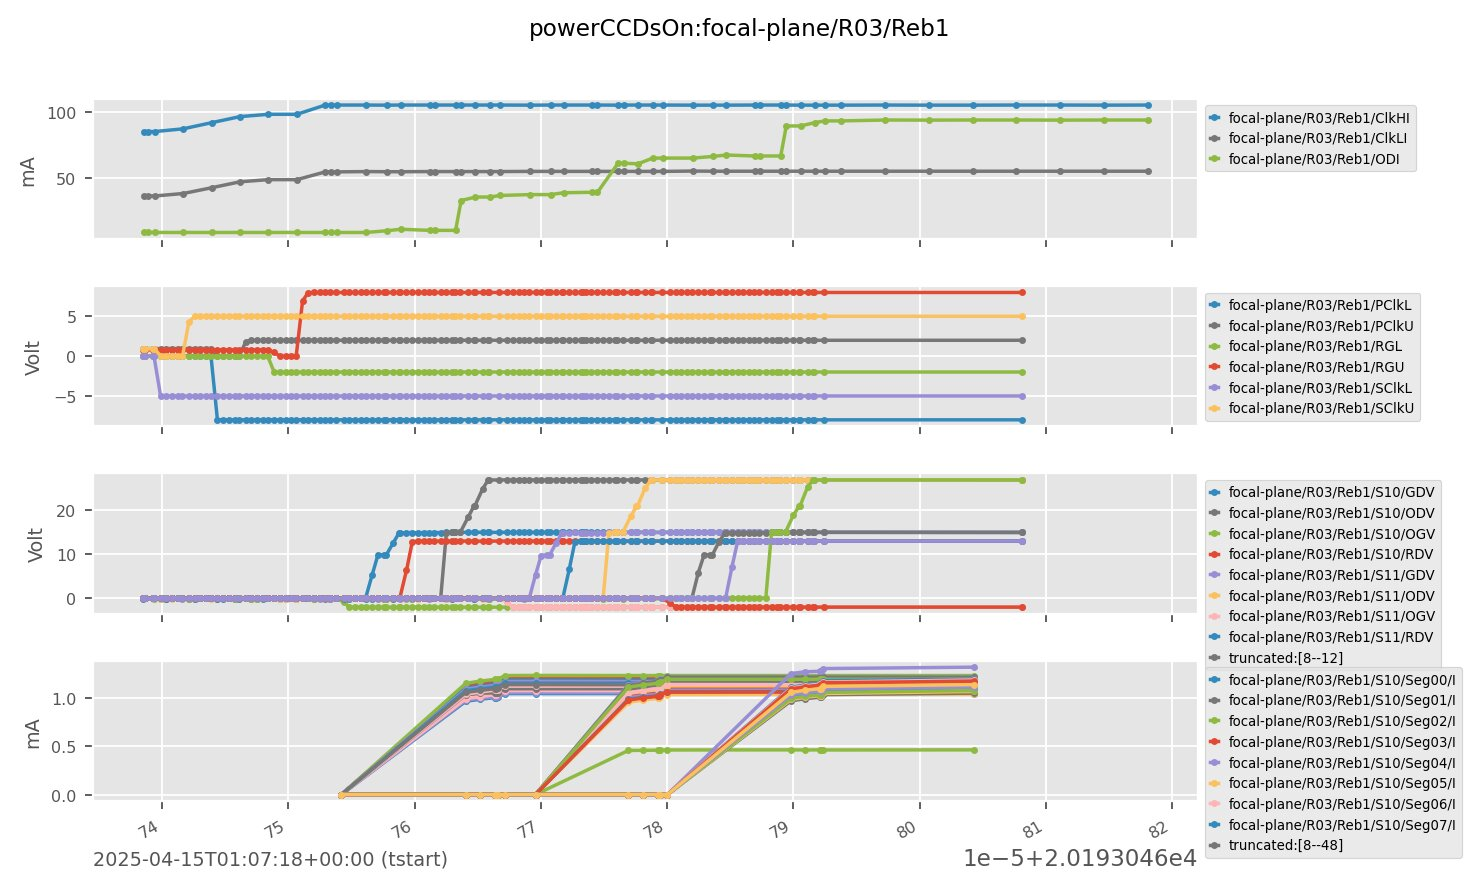
\includegraphics[width=0.62\textwidth]{issues2025/figs/FP-04-a.jpg}
\caption{\textbf{FP-04.} R03/Reb1 being powered on, 15 April.  In the bottom panel every segment current rises to about 1.2\,mA except one, which stays flat: S11/Seg00, the channel that has gone back and forth for years and did not come back this time either (2025-04-15, \#cam-operator).}
\label{fig:iss-FP-04}
\end{figure}

\item[FP-05]\label{iss:FP-05} \textbf{Corner-raft and wavefront-REB power-on workarounds.}
  \emph{First to last mention 2025-04-29 to 2025-10-21; status \textcolor{stwrk}{\textbf{Workaround}}.}
  Corner rafts do not reach the correct dphi level on power-on and need an undocumented DAC-toggle workaround (\rubintkt{LSSTCAM-107}), and a wavefront REB power-on failure requiring a REB power cycle recurred after the October shutdown (\rubintkt{LSSTCAM-37}).  Both were still being worked around at year end rather than fixed.

\item[FP-06]\label{iss:FP-06} \textbf{REB power-supply trips suspected to be electrostatic discharge.}
  \emph{First to last mention 2025-01-21 to 2026-02-16; status \textcolor{stopn}{\textbf{Open}}.}
  Recalled in January: in September 2024 there had been one or two REB power-supply trips that seemed to correlate with people touching or standing near the utility trunk, which is what put the camera-door grounding question (MEC-04) on the agenda in the first place.  A concrete case followed on April~29, when R21/Reb0 tripped during carbon-snow cleaning of M2 with no light-leak explanation and was tentatively attributed to an electrostatic discharge.  The investigation is tracked in the dedicated channel \#cam-issues-esd.  Four more REB power-supply trips in February, still unexplained.  The much larger event of July~7 is registered separately as PWR-02. The door interface a permanent strap has to use is shown in Figure~\ref{fig:iss-MEC-04}.

\end{description}

\noindent\textit{REB firmware}
\begin{description}
\item[FW-01]\label{iss:FW-01} \textbf{REB firmware applying maximum heater power.}
  \emph{First to last mention 2025-08-11 to 2025-08-23; status \textcolor{stres}{\textbf{Resolved}}.}
  The firmware booted during the August~11 recovery made the CCDs run measurably warmer, which was initially misread as lost cryo capacity during the storm.  Power-cycling the focal plane and rolling the firmware back confirmed a real power-draw increase of roughly 30\,W, and the cause was a register-map conflict in 0x313a5013 that applied maximum heater power --- a defect introduced together with the sequencer-override register in 0x31395011 and unnoticed until then.  It was fixed by the firmware upgrade to 0x313a5014. See the version history in Table~\ref{tab:science_reb_fw_en}.

\begin{figure}[H]
\centering
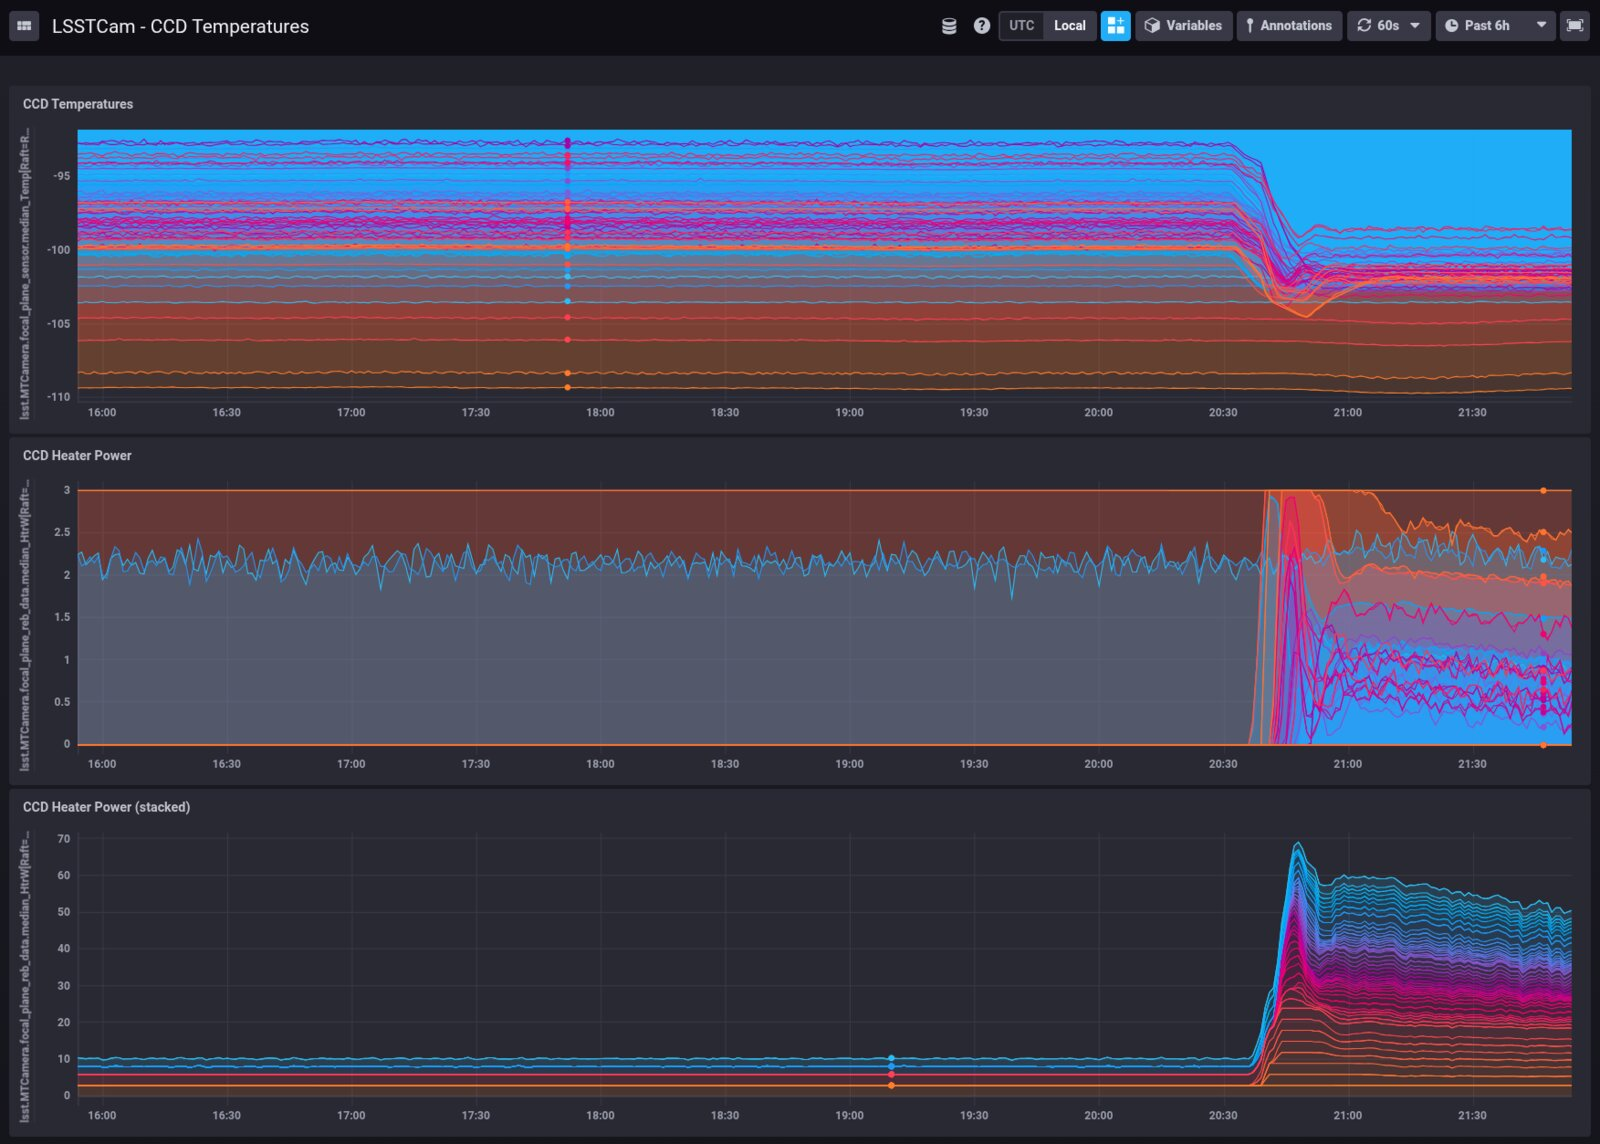
\includegraphics[height=5.63cm]{issues2025/figs/FW-01-a.jpg}\hfill
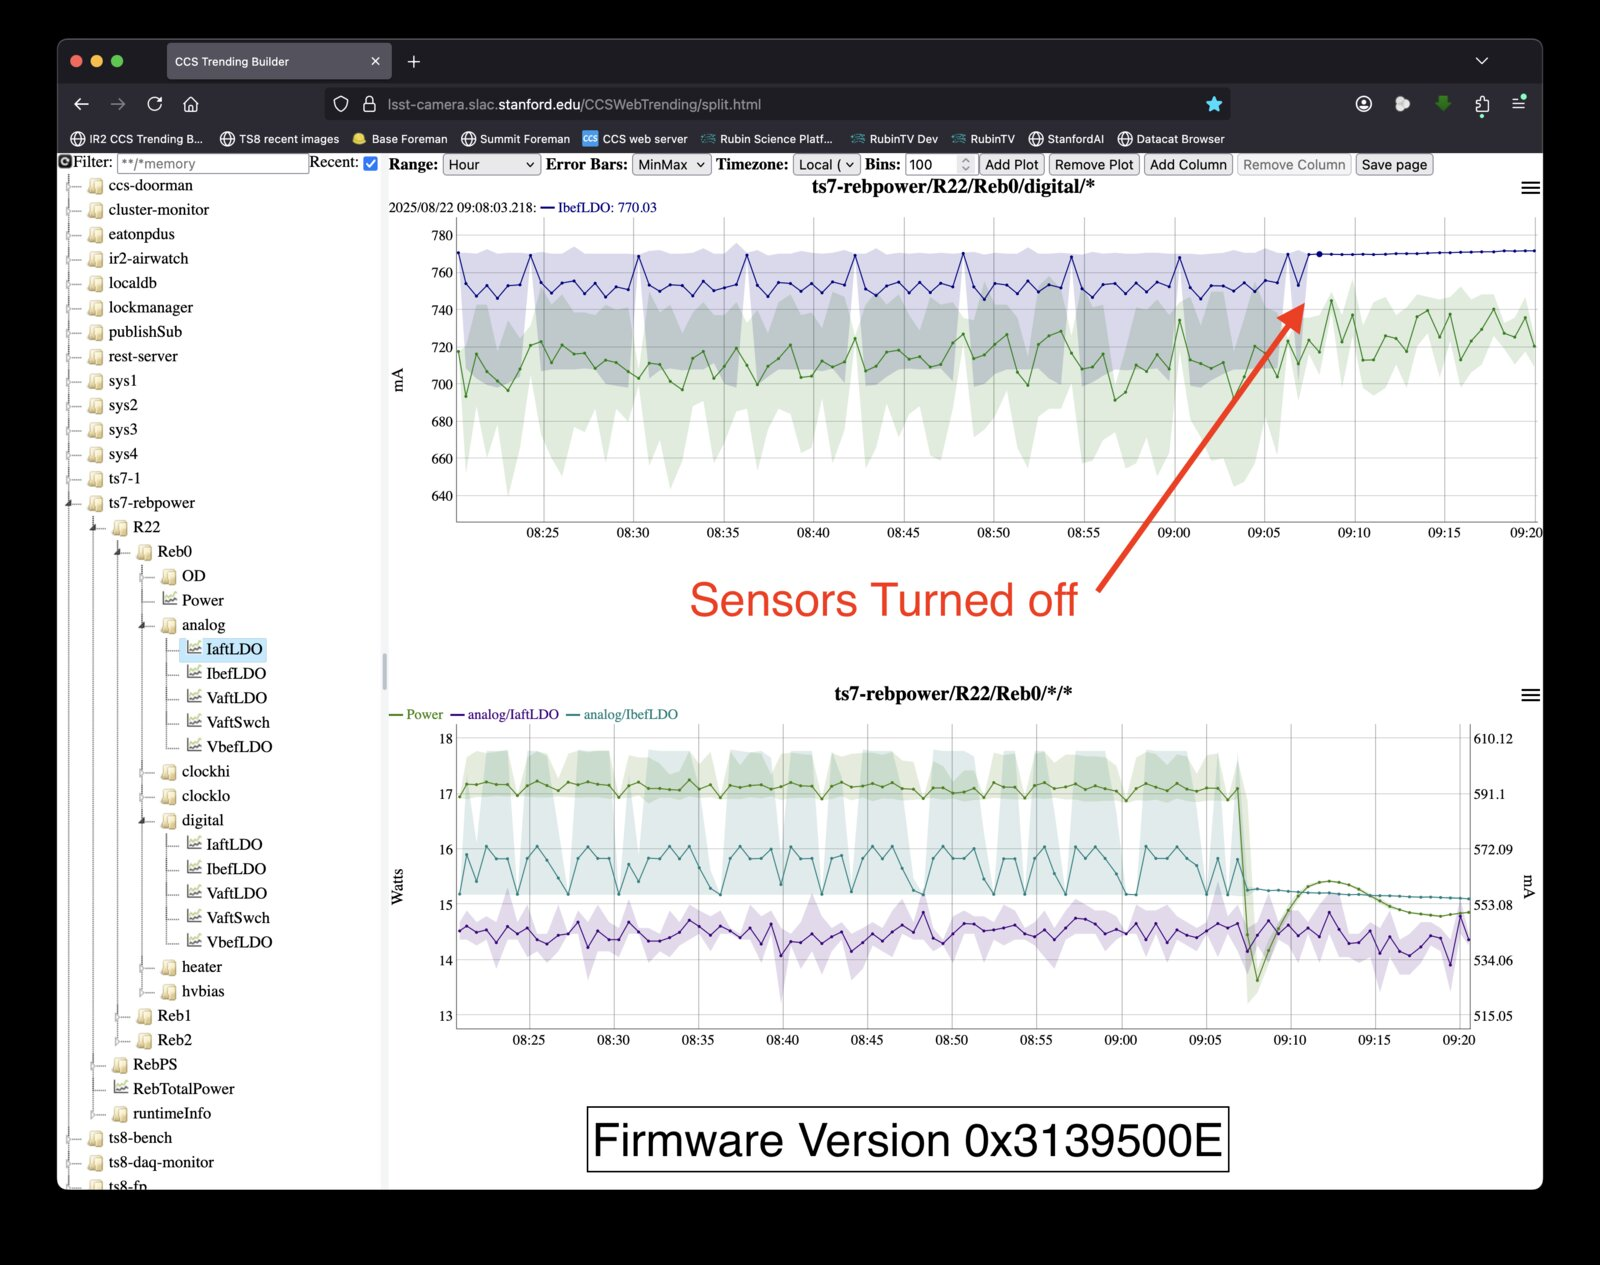
\includegraphics[height=5.63cm]{issues2025/figs/FW-01-b.jpg}
\caption{\textbf{FW-01.} Left: CCD temperatures and CCD heater power across the firmware rollback, the step in heater power being the extra draw the faulty build was applying (2025-08-21).  Right: the same measurement annotated during the investigation, with the moment the sensors were turned off marked and the firmware version under test named (2025-08-22).}
\label{fig:iss-FW-01}
\end{figure}

\item[FW-02]\label{iss:FW-02} \textbf{REB serial-number read race leaving REBs INVALID.}
  \emph{First to last mention 2025-10-13 to 2026-06-25; status \textcolor{stopn}{\textbf{Open}}.}
  Whenever REBs are power-cycled or booted from a different firmware slot, some come back reporting a serial number of zero and stay in an invalid validation state, requiring link resets or RCE reboots before they can be used.  It appeared with the October candidate-firmware rollout and recurred through every subsequent power cycle to the end of the year; tooling improvements (single-RCE reboot, a re-initialize command) were proposed but not delivered.  Unchanged, and now understood: the old wavefront-REB firmware reads the identifier before its clock has settled.  Corrected firmware exists but ``has not been blessed'', so the fix is still to power-cycle the board or restart the focal plane, which was done repeatedly through 2026.

\begin{figure}[H]
\centering
\begin{minipage}{\textwidth}
\hrule\vspace{4pt}
\begingroup\scriptsize
\begin{verbatim}
-- 2025-10-13 19:10 and 21:26 UTC, after the candidate-firmware rollout, #cam-operator

R01/Reb1: CCDsPowerState:OFF HVBiasState:OFF RebDeviceState:ONLINE RebValidationState:INVALID
R01/Reb2: CCDsPowerState:OFF HVBiasState:OFF RebDeviceState:ONLINE RebValidationState:INVALID
R30/Reb1: CCDsPowerState:OFF HVBiasState:OFF RebDeviceState:ONLINE RebValidationState:INVALID
R31/Reb1: CCDsPowerState:OFF HVBiasState:OFF RebDeviceState:ONLINE RebValidationState:INVALID
R32/Reb1: CCDsPowerState:OFF HVBiasState:OFF RebDeviceState:ONLINE RebValidationState:INVALID

-- 2025-11-04 15:31 UTC: the standing recovery, written out for the night crew

Check ID:
rms_read camera 0x800001
Re-read ID:
rms_write camera 0x800000 1
Reset opcode error:
rms_write camera 0x390001 1

-- "Reading 0x800000 shows you the IDs, the firmware bug means that sometimes they come up
--  0x00000000.  If they do, you can cause the REB to re-read the ID by writing 1 to 0x800001."
\end{verbatim}
\endgroup
\vspace{-10pt}\hrule
\end{minipage}
\caption{\textbf{FW-02.} REBs online but refusing validation after a power cycle, and the register recipe that became the standing workaround.  The identifier read is a firmware race, not a hardware fault: the board is reachable, it simply reports a serial number of zero until it is told to read it again.  No fix was delivered in 2025.}
\label{fig:iss-FW-02}
\end{figure}

\item[FW-03]\label{iss:FW-03} \textbf{Sequencer opcode errors after RCE reset.}
  \emph{First to last mention 2025-10-09 to 2026-05-18; status \textcolor{stopn}{\textbf{Open}}.}
  REBs reset or power-cycled while idle clear was running came up with the sequencer opcode-error bit set, needing a register write to clear.  Delaying the start of idle clear until the subsystem is operational was adopted as the mitigation, but the error recurred at the end of December with idle clear confirmed off, pointing at a firmware or boot-sequence cause instead (\rubintkt{LSSTCAM-153}).  Open.  Still recurring on every RCE reset, still cleared by hand.

\begin{figure}[H]
\centering
\begin{minipage}{\textwidth}
\hrule\vspace{4pt}
\begingroup\scriptsize
\begin{verbatim}
-- 2025-12-14 20:17 UTC, #cam-operator, after an RCE restart with idle clear disabled

The RCE restart left three issues. Disabling the idle clear didn't resolve all the issue.

2 Links went down
R22/Reb0: CCDsPowerState:UNKNOWN HVBiasState:UNKNOWN RebDeviceState:OFFLINE RebValidationState:UNKNOWN
R23/Reb2: CCDsPowerState:UNKNOWN HVBiasState:UNKNOWN RebDeviceState:OFFLINE RebValidationState:UNKNOWN

3 REBs have DELTA state in the CCD power
R13/Reb2: CCDsPowerState:DELTA HVBiasState:ON RebDeviceState:ONLINE RebValidationState:VALID
R14/Reb0: CCDsPowerState:DELTA HVBiasState:ON RebDeviceState:ONLINE RebValidationState:VALID
R34/Reb2: CCDsPowerState:DELTA HVBiasState:ON RebDeviceState:ONLINE RebValidationState:VALID

1 opcode error in rms_read
R43/Reb1
\end{verbatim}
\endgroup
\vspace{-10pt}\hrule
\end{minipage}
\caption{\textbf{FW-03.} The observation that reopened the issue.  Idle clear --- the mitigation adopted earlier in the year --- was confirmed off, and an RCE restart still produced a sequencer opcode error, which points the cause at the firmware or the boot sequence rather than at idle clear (\rubintkt{LSSTCAM-153}).}
\label{fig:iss-FW-03}
\end{figure}

\item[FW-04]\label{iss:FW-04} \textbf{Sequencer optimization and the 6.4 ns natural-frequency firmware.}
  \emph{First to last mention 2025-04-26 to 2026-05-11; status \textcolor{stres}{\textbf{Resolved}}.}
  A year-long programme rather than a fault: new sequencer files to address e2v noise and covariance anomalies (clear improvement on e2v, little change on ITL), the 3\,s readout sequencers, and finally the retuning of the sequencer clock to 6.4\,ns.  The natural-frequency firmware was tested on the summit in December in three campaigns and used for a holiday calibration run, but was not promoted to the default slot; the dense photon-transfer curve that these changes require was repeatedly deferred through the year.  The programme was closed in early January 2026, after the period covered here.  The 6.4\,ns firmware went to the whole focal plane on 2026 January~27.  It then produced the sharpest self-inflicted incident of the year: after a power cycle on February~17 the REBs came up with the jitter-cleaner chip left on, drawing about 60\,W more and running 6--7\,$^{\circ}$C hotter, because the build inherited that state instead of setting it.  The camera fell back to the 10\,ns firmware for the night and a corrected build was on the whole camera by the evening of the 18th.  The wavefront sensors were not converted: their testing was canceled in March for want of dark time and a May trial was reverted.

\begin{figure}[H]
\centering
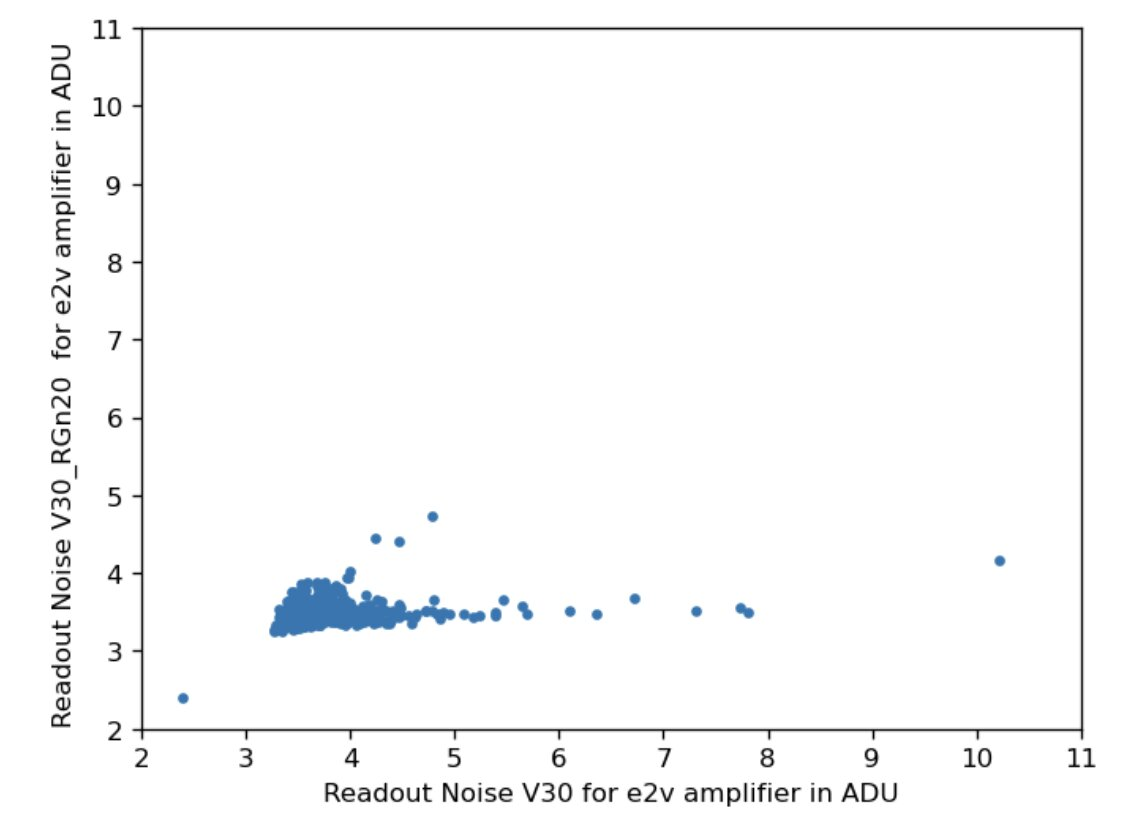
\includegraphics[height=6.31cm]{issues2025/figs/FW-04-a.jpg}\hfill
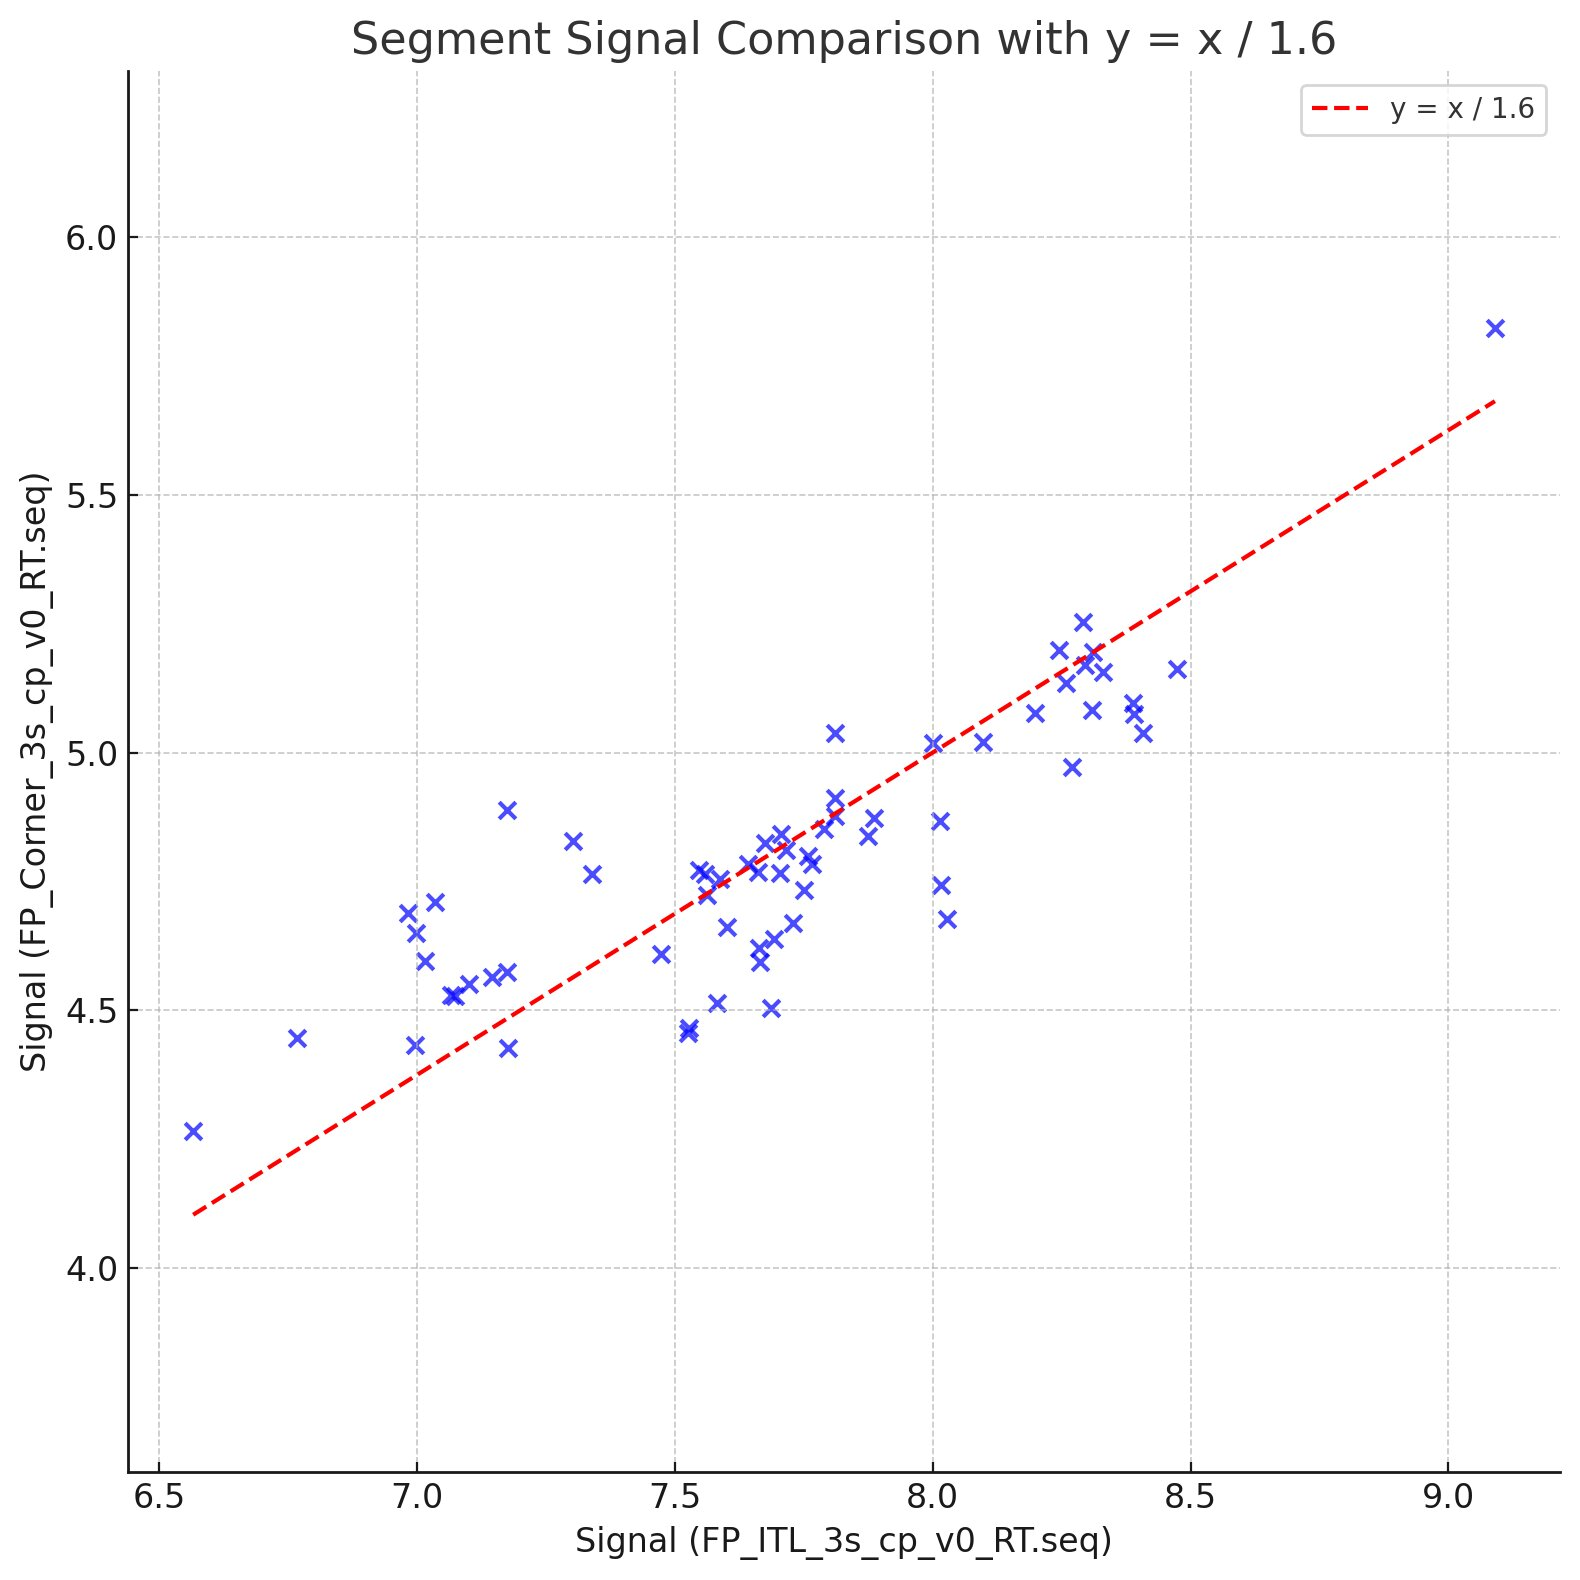
\includegraphics[height=6.31cm]{issues2025/figs/FW-04-b.jpg}
\caption{\textbf{FW-04.} Left: read noise per e2v amplifier with the new sequencer against the old one --- most amplifiers unchanged, the worst improved (2025-04-28).  Right: segment signal with the 3\,s corner-raft sequencer against the ITL one, compared with the expected ratio (2025-06-25).}
\label{fig:iss-FW-04}
\end{figure}

\end{description}

\noindent\textit{Data acquisition}
\begin{description}
\item[DAQ-01]\label{iss:DAQ-01} \textbf{Crate, RCE and data-node crashes.}
  \emph{First to last mention 2025-03-24 to 2026-06-27; status \textcolor{stopn}{\textbf{Open}}.}
  A steady background of DAQ hardware and host faults: bad B-side links traced to DAQ transceivers (March, fixed), memory failures on the data-collection nodes (\rubintkt{OBS-859}), crashed storage and switch-controlling RCEs (\rubintkt{OBS-1208}), a data-transport module needing rebooting twice in a month (\rubintkt{LSSTCAM-130}), and links auto-negotiating down or dropping packets (\rubintkt{LSSTCAM-151}).  Individual instances were cleared by reboots and reseating; the recurrence rate was not.  A serial console was subsequently connected to the worst offender to allow it to be debugged, as documented in \rubintkt{IHS-9431}.  The background rate is unchanged.  The January~19 crash lost a whole data-collection board mid-night and was recognized as the same failure as \rubintkt{OBS-1208} (\rubintkt{OBS-1538}); on April~27 the data-transport modules stopped talking to the DAQ and took the HV and the sensors down with them (\rubintkt{LSSTCAM-171}), again without a cause.

\begin{figure}[H]
\centering
\begin{minipage}{\textwidth}
\hrule\vspace{4pt}
\begingroup\scriptsize
\begin{verbatim}
-- lsstcam-dc06 kernel log, 2025-04-21 03:12 UTC, found during the 1 May investigation
-- and posted to #cam-operator

[Mon Apr 21 03:12:16 2025] {1}[Hardware Error]: Hardware error from APEI Generic Hardware Error Source:
        8
[Mon Apr 21 03:12:16 2025] {1}[Hardware Error]: event severity: corrected
[Mon Apr 21 03:12:16 2025] {1}[Hardware Error]:  fru_text: DIMM_A8
[Mon Apr 21 03:12:16 2025] {1}[Hardware Error]:   section_type: memory error
[Mon Apr 21 03:12:16 2025] {1}[Hardware Error]:    error_status: Storage error in DRAM memory
        (0x0000000000040400)
[Mon Apr 21 03:12:16 2025] {1}[Hardware Error]:   physical_address: 0x0000001e772bb000
[Mon Apr 21 03:12:16 2025] {1}[Hardware Error]:   node:0 card:4 module:1 rank:2 bank:9 row:61369
        column:512
[Mon Apr 21 03:12:16 2025] {1}[Hardware Error]:   error_type: 2, single-bit ECC
[Mon Apr 21 03:12:16 2025] mce: [Hardware Error]: Machine check events logged
\end{verbatim}
\endgroup
\vspace{-10pt}\hrule
\end{minipage}
\caption{\textbf{DAQ-01.} One of the hardware faults behind this entry: a corrected single-bit ECC error on a data-collection node, recorded 10 days before anyone went looking for it.  Faults of this class were cleared individually --- reseating, reboots, transceiver swaps --- but the rate at which they arrived was not addressed.  A serial console was later connected to the worst offender so that it could be debugged when it next fell over (\rubintkt{IHS-9431}).}
\label{fig:iss-DAQ-01}
\end{figure}

\item[DAQ-02]\label{iss:DAQ-02} \textbf{Dropped guider stamps at high ROI rates.}
  \emph{First to last mention 2025-10-10 to 2025-10-13; status \textcolor{stmit}{\textbf{Mitigated}}.}
  Stress-testing large guider regions of interest with the new DAQ release repeatedly dropped guider stamps on the path from the DAQ to \texttt{lsstcam-dc10}, the host that receives and writes them, and the same episodes coincided with dropped group-communication messages.  Extensive network diagnosis of the ATCA switches and the backplane found no definitive cause; the GDS socket buffers were enlarged to 16\,MB and a buffer monitor was run on \texttt{lsstcam-dc10}, after which a 20-image run completed with no dropped packets.

\begin{figure}[H]
\centering
\begin{minipage}{\textwidth}
\hrule\vspace{4pt}
\begingroup\scriptsize
\begin{verbatim}
-- 2025-10-10 18:59--19:15 UTC, guider stress test on lsstcam-dc10, #cam-operator

  "I just took one image MC_C_20251010_000004.  It seems that there were some dropped stamps."

  "N_STAMPS" : 139,   "N_STAMPS" : 138,   "N_STAMPS" : 139,   "N_STAMPS" : 139,
  "N_STAMPS" : 138,   "N_STAMPS" : 136,   "N_STAMPS" : 139,   "N_STAMPS" : 139,

  ("There should have been 139 stamps in that series.")

[2025-10-10T18:59:30.132+0000] WARNING: MC_C_20251010_000004: DAQ stamp count 139 not equal to number
        of stamps received 138 (org.lsst.ccs.daq.guider.FitsWriterFactory$FitsWriter fixupStampCount)
[2025-10-10T18:59:30.174+0000] WARNING: MC_C_20251010_000004: DAQ stamp count 139 not equal to number
        of stamps received 138
[2025-10-10T18:59:30.174+0000] WARNING: MC_C_20251010_000004: DAQ stamp count 139 not equal to number
        of stamps received 136

-- after a buffer monitor was put on the receiving host, 35 minutes later: "That time they all had 139."
\end{verbatim}
\endgroup
\vspace{-10pt}\hrule
\end{minipage}
\caption{\textbf{DAQ-02.} The loss counted at the receiving end.  The DAQ reports how many stamps it sent and the image handler reports how many it wrote, and the two do not agree --- by one to three stamps per sensor per series.  Enlarging the GDS socket buffers to 16\,MB and watching them on \texttt{lsstcam-dc10} removed the loss without ever identifying where it occurred.}
\label{fig:iss-DAQ-02}
\end{figure}

\end{description}

\noindent\textit{Camera Control System}
\begin{description}
\item[CCS-01]\label{iss:CCS-01} \textbf{Guider state desynchronization and focal-plane hangs.}
  \emph{First to last mention 2025-05-01 to 2026-07-06; status \textcolor{stmit}{\textbf{Mitigated}}.}
  The guider state held by CCS and by the DAQ drift apart --- from dangling initialization commands, double commanding between CCS and OCS, or new pause timeouts --- leaving the guider stuck paused (once for 22 hours, unnoticed, with no guider data written) or the focal-plane subsystem hung in an active command state needing a restart.  Individual manifestations were patched repeatedly; the pattern was still recurring on multiple nights in late November (\rubintkt{LSSTCAM-148}).  Two real causes were found in 2026 and the rate came down.  The first was physical: a frame error rate of about $10^{-5}$ on the fiber between the DAQ and the control system, cured by cleaning both ends on February~24 --- ``There have been no Ethernet frame errors since this morning's cleaning'' (\rubintkt{LSSTCAM-151}, \rubintkt{IHS-9679}).  The second was self-inflicted: the guider pause timeout had been switched off after an incident in October 2025, which is what lets the two sides drift apart after a dangling \texttt{initGuiders} (\rubintkt{LSSTCAM-178}, \rubintkt{OBS-1909}).  Hangs still happened into July.

\begin{figure}[H]
\centering
\begin{minipage}{\textwidth}
\hrule\vspace{4pt}
\begingroup\scriptsize
\begin{verbatim}
-- 2025-11-24 09:47 UTC, focal-plane log, posted to #cam-operator the same morning

[2025-11-24T09:47:03.412+0000] INFO: Received command from mcm (user mcm): Command(RawCommand)
        initGuiders with 1 argument ({"common":{"rows":400,"cols":400,"integrationTimeMillis":200}, ...
[2025-11-24T09:47:03.455+0000] WARNING: Accepting initGuiders when guiders already in PAUSED state
        (org.lsst.ccs.subsystem.focalplane.Guiding initGuiders)

   ... no command response for the next 46 minutes ...

[2025-11-24T10:33:08.699+0000] SEVERE: Raised Alert CMDFAIL (Command failed) at severity ALARM 1 time.
        Last cause : "Execution of command "initGuiders" failed unexpectedly due to: Guider start
        failed, status -1 (rc=-1 GDS - Command Timeout)". Overall AlertState= ALARM
org.lsst.ccs.command.CommandInvocationException: org.lsst.ccs.CommandHelper$CommandFailedException:
        Exception while executing command, fault state entered: Guider start failed, status -1 (rc=-1
        GDS - Command Timeout)

-- 2025-11-02 03:24 UTC, the same disagreement seen from the operator's side

initGuiders failed
Guider entered unexpected state, expected=PAUSED actual=ERROR
\end{verbatim}
\endgroup
\vspace{-10pt}\hrule
\end{minipage}
\caption{\textbf{CCS-01.} The state disagreement in one place.  CCS accepts an \texttt{initGuiders} for guiders it already believes are paused, gets no answer from the guider, and only declares failure 46 minutes later; 3 weeks earlier the same disagreement surfaced as a state the operator could not act on.  The pattern was still recurring at the end of November (\rubintkt{LSSTCAM-148}).}
\label{fig:iss-CCS-01}
\end{figure}

\item[CCS-02]\label{iss:CCS-02} \textbf{Idle clear: from guider clearing noise to default operation.}
  \emph{First to last mention 2025-04-16 to 2025-07-04; status \textcolor{stres}{\textbf{Resolved}}.}
  Guider idle-clearing was found in April to inject noise into neighbouring sensors during bias readout, making early bias images unusable and producing stripes in wavefront images (\slactkt{LSSTCCSRAFTS-778}).  The proper fix --- a non-guider idle-clear scheme --- arrived with CCS 41.0.4 in late June, needed two further locking fixes (skipped invocations piling up, and a sequencer-reload race that showed up as a runaway clock current on R30/Reb2), and was declared operational on June~30.  Idle clear has been the default for all on-sky observations since early July, replacing continuous all-day biases.

\begin{figure}[H]
\centering
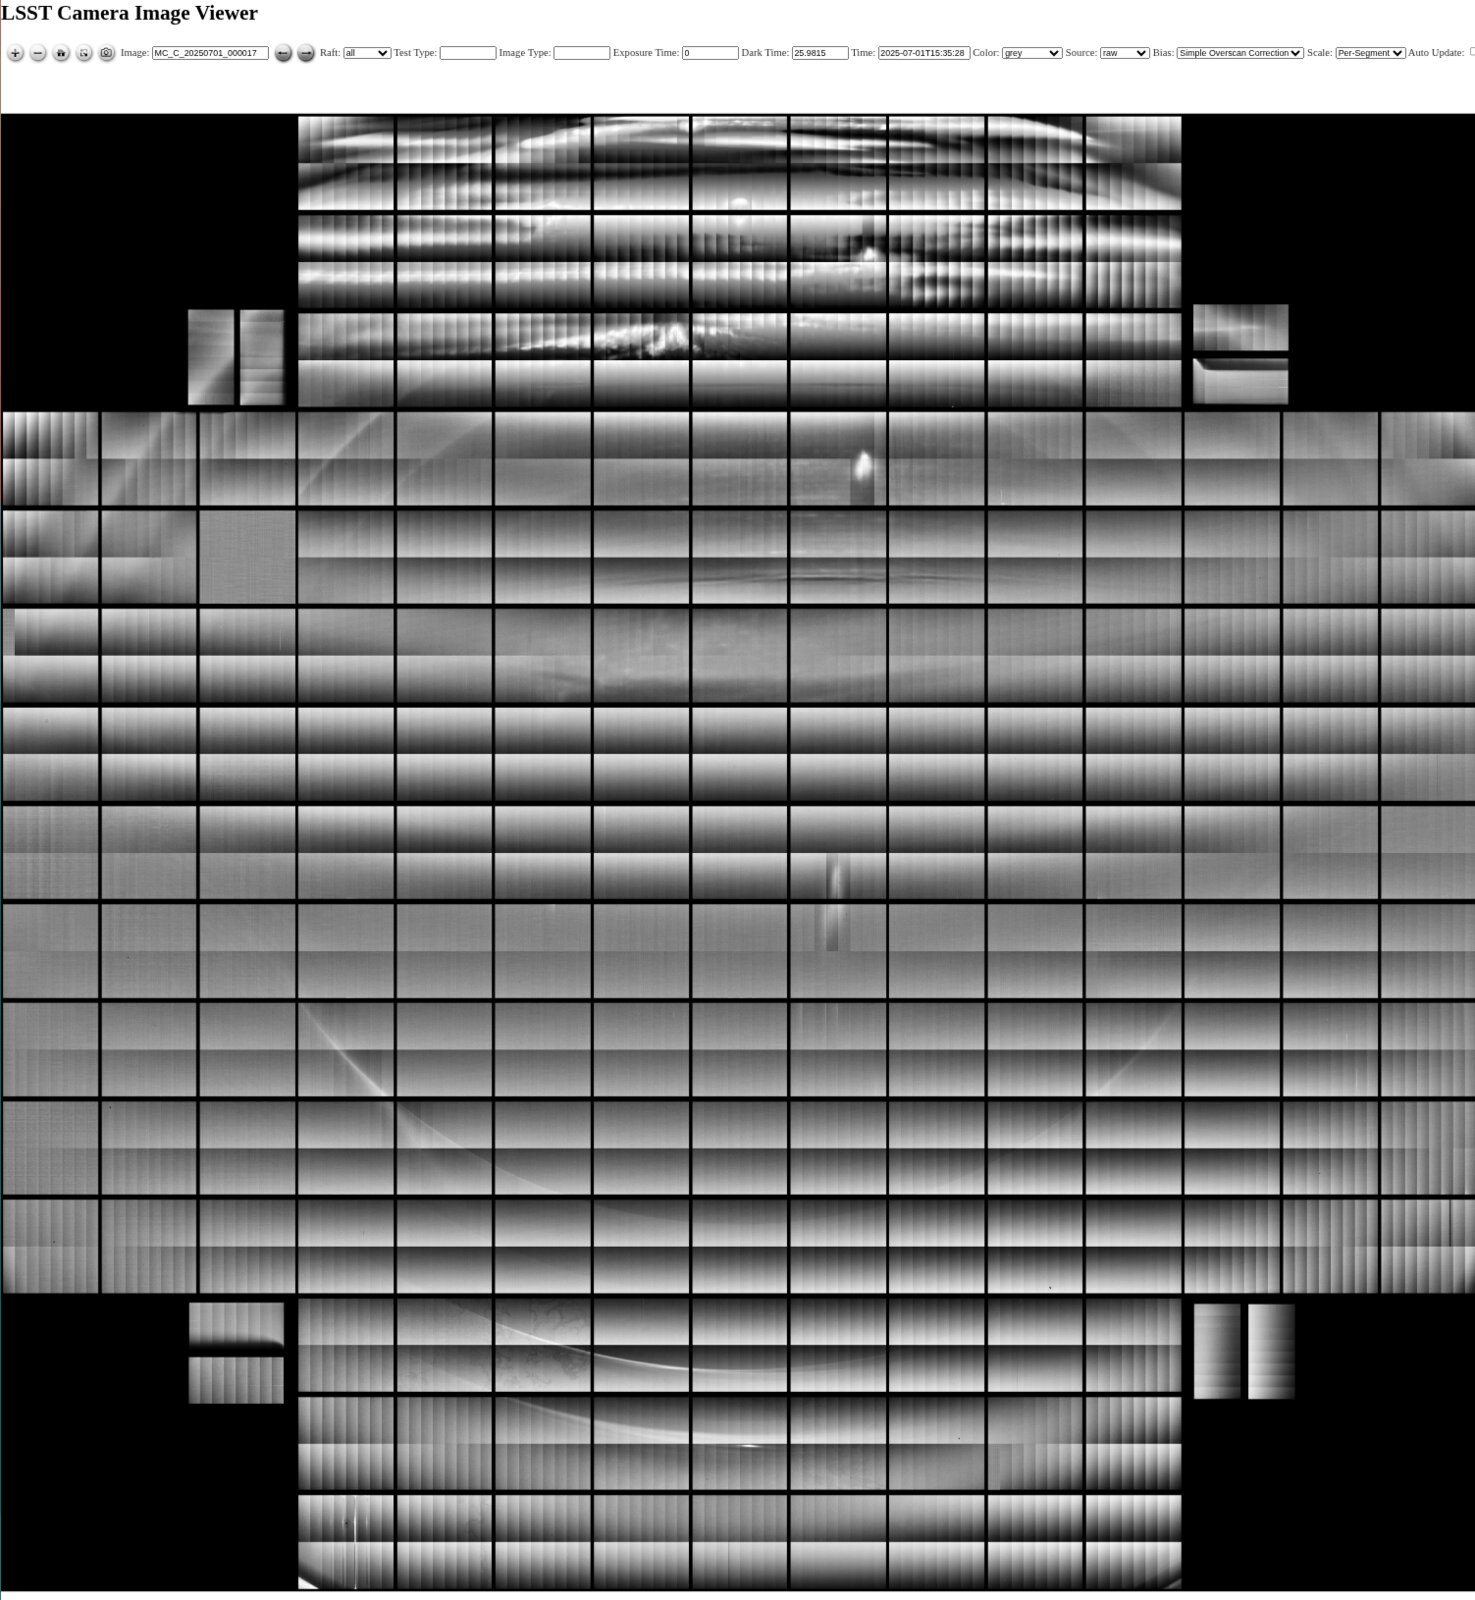
\includegraphics[width=0.62\textwidth]{issues2025/figs/CCS-02-a.jpg}
\caption{\textbf{CCS-02.} A bias exposure with the guider running: the structure across the upper rafts is the artefact that idle clear was introduced to remove (2025-07-01).}
\label{fig:iss-CCS-02}
\end{figure}

\item[CCS-03]\label{iss:CCS-03} \textbf{ocs-bridge failures to release the mount motion lock.}
  \emph{First to last mention 2025-07-13 to 2025-11-09; status \textcolor{stopn}{\textbf{Open}}.}
  After a filter change the bridge between CCS and the observatory control system intermittently fails to acknowledge the unlock command to the mount and rotator, leaving them motion-locked and the filter command rejected (\rubintkt{OBS-1098}, \rubintkt{OBS-1079}, \rubintkt{OBS-1119}, \rubintkt{OBS-1360}).  A SAL interface version mismatch is suspected.  The standing recovery is to take the camera offline and restart the bridge; it cost whole nights in July and recurred in November.

\begin{figure}[H]
\centering
\begin{minipage}{\textwidth}
\hrule\vspace{4pt}
\begingroup\scriptsize
\begin{verbatim}
-- 2025-04-30 02:40 UTC, ocs-bridge log, posted to #cam-operator

[2025-04-30T02:39:51.323+0000] INFO: MTRotator MotionLockStateEvent MotionLockStateEvent{lockState=2,
        identity=Script:100003}
[2025-04-30T02:39:55.421+0000] INFO: MTRotator MotionLockStateEvent MotionLockStateEvent{lockState=0,
        identity=Script:100003}
[2025-04-30T02:40:22.490+0000] INFO: Received command: SetFilterCommand{name=g_6}
[2025-04-30T02:40:22.491+0000] INFO: Sending MTRotator: LockMotionCommand{}
[2025-04-30T02:40:26.601+0000] INFO: Command complete ack=303
[2025-04-30T02:40:26.601+0000] INFO: Sending MTMount: LockMotionCommand{}
[2025-04-30T02:40:26.603+0000] INFO: MTRotator MotionLockStateEvent MotionLockStateEvent{lockState=3,
        identity=ocs-bridge}
[2025-04-30T02:40:26.627+0000] SEVERE: Command failed: errorCode=1, ack=-302, message=Failed: Currently
        <MotionLockState.UNLOCKING: 2>. Cannot lock motion.
[2025-04-30T02:40:26.627+0000] SEVERE: Failed to get motion lock during setFilter command
[2025-04-30T02:40:26.627+0000] INFO: Reject command: SetFilterCommand{name=g_6} because Command
        rejected: Failed: Currently <MotionLockState.UNLOCKING: 2>. Cannot lock motion.

-- and from the CCS console a quarter of an hour later

 ccs>fcs setFilter 6
Error: Error dispatching command: The telescope motion and rotator need to be locked before
performing a filter exchange. Current status of the lock is UNLOCKED
\end{verbatim}
\endgroup
\vspace{-10pt}\hrule
\end{minipage}
\caption{\textbf{CCS-03.} A filter change refused because the mount is stuck between lock states.  The rotator reports \texttt{UNLOCKING} when the bridge tries to lock it, the \texttt{setFilter} command is rejected, and the console shows the same lock reported as \texttt{UNLOCKED}.  Recovery on this night needed the MTMount CSC to be cycled.}
\label{fig:iss-CCS-03}
\end{figure}

\item[CCS-04]\label{iss:CCS-04} \textbf{Vacuum-subsystem fault that silently disabled a safety interlock.}
  \emph{First to last mention 2025-02-25 to 2025-03-04; status \textcolor{stmit}{\textbf{Mitigated}}.}
  In February a vacuum-subsystem fault left seven MKS gauges --- including the safety-critical cryostat and heat-exchanger (Hx) gauges --- offline for over 15 hours and aborted the low-vacuum check, so the refrigeration-not-permitted alarm was never re-raised despite high pressures: protection remained nominally configured while not working.  The defect was fixed under \slactkt{LSSTCCSSUB-212} and the corrected build was installed by hand on the summit in early March.

\begin{figure}[H]
\centering
\begin{minipage}{\textwidth}
\hrule\vspace{4pt}
\begingroup\scriptsize
\begin{verbatim}
-- 2025-02-25 19:31--19:37 UTC, vacuum subsystem log, posted to #cam-operator

[2025-02-25T18:09:58.533+0000] SEVERE: Setting ASM380 offline due to error retrieving initial status
        ASM380: org.lsst.ccs.drivers.commons.DriverException: Device not connected
        (org.lsst.ccs.subsystem.vacuum.ASM380Device initialize)

-- and, from the subsystem restart the previous evening:

java.lang.NullPointerException: Name is null
        at java.base/java.lang.Enum.valueOf(Enum.java:271)
        at org.lsst.ccs.subsystem.vacuum.constants.DeviceState.valueOf(DeviceState.java:11)
        at org.lsst.ccs.subsystem.vacuum.VacuumMain.updateCryoTurboPumpVentValve(VacuumMain.java:1118)
        at org.lsst.ccs.subsystem.vacuum.VacuumMain.updateSwitchState(VacuumMain.java:976)
        at org.lsst.ccs.subsystem.vacuum.VacuumMain.updateVacuumState(VacuumMain.java:676)
        at org.lsst.ccs.services.PeriodicTaskComponent$PeriodicTaskRunnableWrapper.run(PeriodicTaskCompo
        nent.java:205)
        at org.lsst.ccs.utilities.scheduler.PeriodicTask.run(PeriodicTask.java:186)
[2025-02-24T21:05:33.518+0000] SEVERE: Exception thrown by periodic task vacuum-state
        (org.lsst.ccs.utilities.scheduler.PeriodicTaskExceptionHandler onException)
\end{verbatim}
\endgroup
\vspace{-10pt}\hrule
\end{minipage}
\caption{\textbf{CCS-04.} The February fault as it appears in the log.  Devices are set offline at subsystem start-up and the \texttt{vacuum-state} periodic task --- the task that evaluates the pressures and raises \texttt{RefrigNotPermitted} --- dies on a null device state.  Seven MKS gauges, including the cryostat and heat-exchanger gauges, stayed offline for more than 15 hours; the interlock was configured throughout and did nothing.}
\label{fig:iss-CCS-04}
\end{figure}

\item[CCS-05]\label{iss:CCS-05} \textbf{Automatic REB protective shutdown did not fire.}
  \emph{First to last mention 2025-11-20 to 2025-11-20; status \textcolor{stopn}{\textbf{Open}}.}
  During the total Dynalene loss of November~20 the automatic REB shutdown response failed to act, because the REB power-supply board high-temperature limit was set above the value at which the response was expected to intervene, and the camera had to be shut down by hand (\rubintkt{FRACAS-321}).  The high-temperature limit has not been changed since.  Although the event presented as a cooling failure, the defect is in the control system's protective logic and its configuration, which is why it is registered here rather than with the Dynalene issues. The board temperatures this response is meant to act on rise as in the Dynalene events of Figure~\ref{fig:iss-DYN-01}.

\item[CCS-06]\label{iss:CCS-06} \textbf{jGroups multicast storms (``meltdowns'').}
  \emph{First to last mention 2025-02-15 to 2026-04-28; status \textcolor{stmit}{\textbf{Mitigated}}.}
  Retransmit storms on the CCS group-communication layer that break CCS--DAQ communication and, in the worst cases, require nearly every subsystem to be killed and restarted (\rubintkt{OBS-950}).  Several distinct triggers were identified over the year --- a console process hitting its memory limit, IGMP snooping enabled on particular switches, guiding at an untested 5\,s cadence with high DAQ traffic, a locked console, Kafka broker memory exhaustion --- and each was addressed, yet the class of failure recurred in November.  No single root cause was established.  A cause was finally named, twice: a runaway graphical console on an operator workstation, in January (\rubintkt{OBS-1558}) and again on April~28.  ``JGroups is likely a victim in this case.''  A deliberate test in March reproduced a self-sustaining storm that took 35 minutes to clear, and a repeat after the server migration would not reproduce it.

\begin{figure}[H]
\centering
\begin{minipage}{\textwidth}
\hrule\vspace{4pt}
\begingroup\scriptsize
\begin{verbatim}
-- 2025-02-18 17:00 UTC, chiller (refrig) log on lsstcam-pcs02, posted to #cam-operator

Feb 18 17:00:39 lsstcam-pcs02 refrig[2624]: 4561 INFO: [STATUS] NAKACK2: retransmit request from
        CCSAddress s-CCS-Graphical-Console_lsstcam-mcm_FEutSUX uuid=9d3f19e...
Feb 18 17:00:40 lsstcam-pcs02 refrig[2624]: 4562 INFO: [STATUS] NAKACK2: retransmit request from
        CCSAddress s-CCS-Graphical-Console_lsstcam-mcm_FEutSUX uuid=9d3f19e...
Feb 18 17:00:41 lsstcam-pcs02 refrig[2624]: 4563 INFO: [STATUS] NAKACK2: retransmit request from
        CCSAddress s-CCS-Graphical-Console_lsstcam-mcm_FEutSUX uuid=9d3f19e...
Feb 18 17:00:43 lsstcam-pcs02 refrig[2624]: 4564 INFO: [STATUS] NAKACK2: retransmit request from
        CCSAddress s-CCS-Graphical-Console_lsstcam-mcm_FEutSUX uuid=9d3f19e...
Feb 18 17:00:56 lsstcam-pcs02 refrig[2624]: 4567 INFO: [STATUS] NAKACK2: retransmit request from
        CCSAddress s-CCS-Graphical-Console_lsstcam-mcm_FEutSUX uuid=9d3f19e...

-- 2025-04-07 18:39 UTC, mcm log: the other face of the same layer

[2025-04-07T18:39:02.871+0000] WARNING: [STATUS] JGRP000011: s-mcm: dropped message from non-member
        s-image-handling-lsstcam-dc09 (view=[s-camera-mmm|59166] (36) [s-camera-mmm, s-lockmanager,
        s-ocs-bridge, s-mcm, s-cluster-monitor, s-kafkaService, ...]) (org.jgroups.ccs.CCSLog warn)
\end{verbatim}
\endgroup
\vspace{-10pt}\hrule
\end{minipage}
\caption{\textbf{CCS-06.} What a meltdown looks like in the log: an unbroken stream of \texttt{NAKACK2} retransmit requests, here all provoked by a single graphical console, and --- from a different episode --- a subsystem dropped from the group view while it is still running and still sending.  Neither line names a cause, which is the difficulty with this class of failure.}
\label{fig:iss-CCS-06}
\end{figure}

\item[CCS-07]\label{iss:CCS-07} \textbf{Kafka broker and rebpower memory exhaustion.}
  \emph{First to last mention 2025-11-01 to 2026-05-20; status \textcolor{stres}{\textbf{Resolved}}.}
  The Kafka broker service and the REB-power subsystem exhausted their Java memory, the broker reaching extreme CPU use and the subsystem dropping to tens of megabytes free, which triggered an overnight storm (\rubintkt{LSSTCAM-149}, \rubintkt{LSSTCAM-150}).  Restarting both services at the start of each night became standing practice --- a workaround, not a fix.  Fixed on 2026 May~20.  The broker was stopping on a full queue (\rubintkt{LSSTCAM-179}); the defect was found, a workaround patched into the installation on the master control machine, and the nightly restarts stopped being necessary.

\begin{figure}[H]
\centering
\begin{minipage}{\textwidth}
\hrule\vspace{4pt}
\begingroup\scriptsize
\begin{verbatim}
-- 2025-11-23 04:48--04:50 UTC, rebpower and kafkaService logs, posted to #cam-operator

[2025-11-23T04:48:15.803+0000] WARNING: Raised Alert JVM/memory/available (JVM available memory is
        below 50 MB.) at severity WARNING 1 time. Last cause : "PULSE: Low available memory: 32 MB.
        Max: 1979 MB, Allocated: 1979 MB, Used: 1947 MB.". Overall AlertState= WARNING
[2025-11-23T04:48:18.017+0000] INFO: [STATUS] NAKACK2: retransmit request from CCSAddress
        s-kafkaService uuid=eab348cf... for (1): {96968562}
[2025-11-23T04:48:20.754+0000] INFO: [STATUS] NAKACK2: retransmit request from CCSAddress
        s-kafkaService uuid=eab348cf... for (1): {96969728}
[2025-11-23T04:48:49.643+0000] WARNING: REB PS board (192.168.1.53): Read of seqno a0135940 took
        unexpectedly long time 763ms (org.lsst.ccs.drivers.auxelex.Srp receive)
[2025-11-23T04:48:49.644+0000] SEVERE: Periodic task monitor-update/RebPS/P03 did not finish execution
        by the end of its period of 1000 ms. Still runnung. ... GC: G1 Young Generation from 254 to 255
        for 1, G1 Old Generation from 255 to 1017 for 762.
[2025-11-23T04:49:59.230+0000] WARNING: [STATUS] JGRP000011: s-kafkaService: dropped message from
        non-member s-rebpower (view=[s-camera-mmm|80414] (36) [...])
\end{verbatim}
\endgroup
\vspace{-10pt}\hrule
\end{minipage}
\caption{\textbf{CCS-07.} Ninety seconds of the November~23 storm, in order: \texttt{rebpower} down to 32\,MB of its 1979\,MB heap, retransmit requests from the Kafka service, REB power-supply reads taking three quarters of a second, the monitoring task overrunning its 1\,s period in old-generation garbage collection, and finally \texttt{rebpower} dropped from the group view.  The memory exhaustion precedes the communication failure rather than following it (\rubintkt{LSSTCAM-149}, \rubintkt{LSSTCAM-150}).}
\label{fig:iss-CCS-07}
\end{figure}

\item[CCS-08]\label{iss:CCS-08} \textbf{Silent death of periodic tasks.}
  \emph{First to last mention 2025-03-22 to 2026-04-24; status \textcolor{stopn}{\textbf{Open}}\,\textbf{?}.}
  A separate and more general defect than CCS-04: a periodic task stops executing after reaching its maximum allowed number of exceptions and the subsystem carries on as if nothing had happened.  In March a chiller control panel was found frozen, showing the chiller off with the emergency stop asserted while it was in fact running, because the state-update task had died on a null-pointer exception; the resulting failure alert appeared in the log and the alert viewer but did not reach the Slack channels, which is what allowed it to go unnoticed.  A similar periodic-task failure recurred in October.  Whether the general problem was addressed afterwards is not visible in the operations channels.  Twice more, and the second time with the point made plainly: a vacuum monitoring task died after its tenth read failure while the trending went on displaying its last values as though they were live.

\begin{figure}[H]
\centering
\begin{minipage}{\textwidth}
\hrule\vspace{4pt}
\begingroup\scriptsize
\begin{verbatim}
-- 2025-03-22 18:59 UTC, chiller-ccs log of 2025-03-16, retrieved after the panel was
-- found frozen six days later and posted to #cam-operator

ccs-logs-chiller-ccs-20250316.log.0.gz:
[2025-03-16T22:51:52.603+0000] SEVERE: Raised Alert PeriodicTaskFailure (Alert raised when periodic
        tasks have failures (exceptions) during execution. At ALARM level the task execution is
        terminated.) at severity ALARM 1 time. Last cause : "Task updateCtrlState has experenced the
        maximum allowed number of exceptions: 10 (max:10). It has stopped executing.
        ([updateCtrlState])."

-- the exception itself

[2025-03-16T22:51:45.047+0000] SEVERE: Exception thrown by periodic task updateCtrlState
        (org.lsst.ccs.utilities.scheduler.PeriodicTaskExceptionHandler onException)
java.lang.NullPointerException: Cannot invoke "java.lang.Boolean.booleanValue()" because the return
        value of "org.lsst.ccs.subsystem.refrig.ChillerMaq20Device.isLightOn(org.lsst.ccs.subsystem.refr
        ig.ChillerMaq20Device$LightNumber)" is null
\end{verbatim}
\endgroup
\vspace{-10pt}\hrule
\end{minipage}
\caption{\textbf{CCS-08.} The failure mode in full.  A periodic task reaches its allowed number of exceptions, stops executing, and the subsystem goes on serving the last state it managed to write --- here a chiller shown as off with the emergency stop asserted while it was running normally.  The alert was raised on 16~March and the condition was noticed on 22~March: it reached the log and the alert viewer, but not the operations channels.}
\label{fig:iss-CCS-08}
\end{figure}

\item[CCS-09]\label{iss:CCS-09} \textbf{Camera states that nothing alarms on.}
  \emph{First to last mention 2026-06-09 to 2026-07-02; status \textcolor{stmit}{\textbf{Mitigated}}.}
  Twice in 5 weeks the camera was left in a wrong state that no alarm caught.  The back-bias switch on R12/Reb0 was never closed during an HV ramp on June~9 and the raft ran with its HV off for 3 days, noticed by an automated check and, independently, by someone looking at the images.  On July~1 a \texttt{rebpower} restart left the HV regulator in \texttt{IDLE}, so the voltage drifted un-regulated for a night; no science data was lost only because none was taken.  Both were met with procedure --- a line in the operations manual, a request for a displayed count of HV switches on and off --- rather than with an alarm.

\end{description}

\noindent\textit{Shutter}
\begin{description}
\item[SHT-01]\label{iss:SHT-01} \textbf{Shutter blade overrun and stuck states.}
  \emph{First to last mention 2025-03-24 to 2025-10-21; status \textcolor{stres}{\textbf{Resolved}}.}
  The shutter jammed part-open during a flat calibration in June, with the blade apparently overrunning its limit, and was recovered only by power-cycling both PLCs and the HCU and recalibrating (\rubintkt{OBS-1013}).  It stuck again during a 15\,s exposure at a non-zero rotator angle in October, throwing an illegal-duration exception in the controller (\rubintkt{LSSTCAM-135}), and needed reinitialization on the first night back from the shutdown.  An earlier motion-profile study in March had already shown anomalous Hall-sensor transitions and higher jerk than the 2022 reference set.  These stuck and overrun states are accounted for by the shutter timing analysis and were resolved with it. See Section~\ref{sec:shutter-timing}.

\begin{figure}[H]
\centering
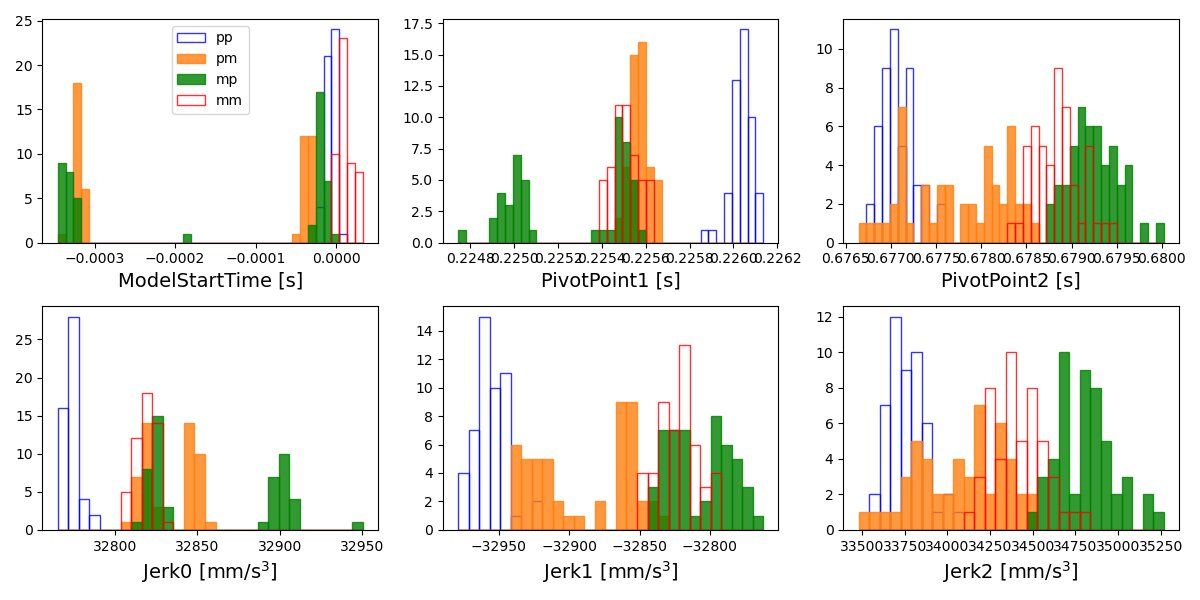
\includegraphics[height=4.07cm]{issues2025/figs/SHT-01-a.jpg}\hfill
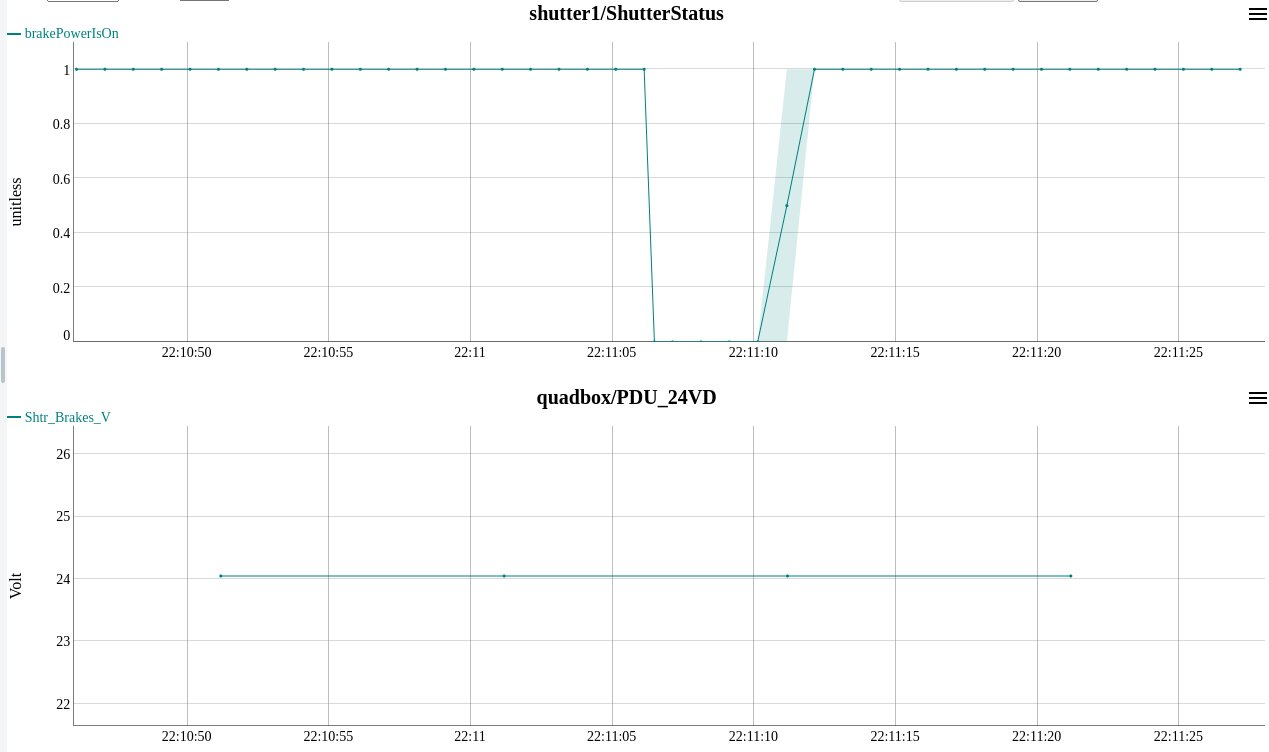
\includegraphics[height=4.07cm]{issues2025/figs/SHT-01-b.jpg}
\caption{\textbf{SHT-01.} Left: the shutter motion-profile study of March, fitting model start time, pivot points and jerk for each blade and comparing them with the 2022 reference set (2025-03-24).  Right: shutter status and the quadbox 24\,V supply across one of the stuck-shutter events (2025-04-23).}
\label{fig:iss-SHT-01}
\end{figure}

\item[SHT-02]\label{iss:SHT-02} \textbf{Shutter PTP time synchronization.}
  \emph{First to last mention 2025-06-04 to 2026-01-21; status \textcolor{stmit}{\textbf{Mitigated}}.}
  Repeated ``timed out waiting for shutter exposure to complete'' failures in June were traced not to the mechanism but to PTP clocking: enabling a boundary clock on the shutter's switch reproduced the fault on the clean-room system, and transparent-clock mode and then the leaf switch as boundary clock removed the offset from master.  The analysis and recovery procedure are documented in \href{https://ctn-003.lsst.io}{CTN-003}.  Synchronization still falls out of lock after major network events.  It did so twice in November: during the recovery from the November~3 jGroups meltdown, where \texttt{readPtpDiag.sh} was run repeatedly from 20:53 to 22:42\,UTC and the offset from master ranged from tens of milliseconds up to 0.96\,s before the shutter was recalibrated in a closed dome, and again on November~20 during the Dynalene recovery, when the shutter was restarted and the synchronization was reported as bad at 19:52\,UTC.  Recovery in both cases required PLC power cycles and recalibration.  The delay chased through January turned out not to be the shutter at all, but guider initialization commands still being issued when guiding was supposed to be off. See Section~\ref{sec:shutter-timing}.

\begin{figure}[H]
\centering
\begin{minipage}{\textwidth}
\hrule\vspace{4pt}
\begingroup\scriptsize
\begin{verbatim}
-- 2025-11-03, recovery from the jGroups meltdown: readPtpDiag.sh on lsstcam-shutter01,
-- run repeatedly between 20:53 and 22:42 UTC.  Two of the readings, unedited except for
-- the lines common to both.

  22:14:25                                   |    22:42:06  (after the network settled)
  PTP state:               SLAVE (9)         |    PTP state:               SLAVE (9)
  Offset from master (ns): 961,800,987       |    Offset from master (ns): 43,082
  Mean path delay (ns):    9,466             |    Mean path delay (ns):    26,598
  Steps removed:           4                 |    Steps removed:           4

-- and the field that shows what the shutter itself believed the time was:

  External (PTP) time:     Wed, 10 Dec 2025 21:58:45.689932 UTC
  (the HCU clock read 2025-11-03 22:14:25 at that moment)
\end{verbatim}
\endgroup
\vspace{-10pt}\hrule
\end{minipage}
\caption{\textbf{SHT-02.} Loss of lock after a network event, in the diagnostic the shutter provides.  An offset from master of 0.96\,s --- against the tens of nanoseconds of a healthy lock --- and a PTP time 5 weeks ahead of the real one; both recover without intervention once the network settles.  This is the November recurrence referred to in the entry; the analysis and the recovery procedure are in \href{https://ctn-003.lsst.io}{CTN-003}.}
\label{fig:iss-SHT-02}
\end{figure}

\end{description}

\noindent\textit{Filter exchange system}
\begin{description}
\item[FES-01]\label{iss:FES-01} \textbf{Carousel clamp faults.}
  \emph{First to last mention 2025-05-02 to 2026-06-15; status \textcolor{stres}{\textbf{Resolved}}.}
  The dominant filter-exchange failure mode: a carousel clamp fails to open or lock within the allowed time, faulting the changer and costing observing time.  It was attacked from three sides --- automated unclamping recovery in July (error rate below 1 in 400 over 1000 exchanges once deployed), servicing and greasing of the socket clamps during the October shutdown, and a warm-up brake sequence in November --- and the rate came down, but socket-specific faults were still occurring in December.  A filter had to be removed from the camera in July when socket~3 could not be trusted.  Closed by the October 2025 maintenance, which is where the cause was found.  All ten clamps were dismounted and greased --- they had not been touched since the 2021 installation --- and the socket~3 clamp was found with bare steel on steel where a coating patch was missing.  Before that the rate had reached roughly one fault a day at the start of July 2025, held off only by an automated unclamping recovery deployed on July~9--11.  After the maintenance: ``No friction in clamps, all sockets in nominal operating condition'' (2025-10-10).  A thousand filter changes in the 2 months that followed produced two stopping errors, against a target of fewer than one intervention in a thousand, and the three thousandth change was reached in February 2026.  Socket~1 went on asking for an occasional recovery; a software mitigation for it --- a short pulse of unlock current after release --- was tested successfully on 2026 June~15.

\item[FES-02]\label{iss:FES-02} \textbf{Carousel socket 3 slip-ring collector.}
  \emph{First to last mention 2025-04-13 to 2025-04-25; status \textcolor{stres}{\textbf{Resolved}}.}
  Socket~3 lost communication intermittently during carousel rotation, worse at speed and dependent on telescope orientation.  The cause was a spring-loaded carbon collector contact that was not sliding freely; it was replaced on April~24--25 and the socket recovered (\rubintkt{SUMMIT-10680}).  The eight untouched collectors, and the effect of the very dry camera atmosphere on them, were noted as a residual risk.

\item[FES-03]\label{iss:FES-03} \textbf{Autochanger trucks, homing and the damaged X+ clamp motor.}
  \emph{First to last mention 2025-02-13 to 2026-07-09; status \textcolor{stmit}{\textbf{Mitigated}}.}
  The autochanger truck controllers fault with undervoltage errors after losing homing, a problem that first blocked filter exchange in February and reappeared in December (\rubintkt{OBS-1454}); a new automated homing procedure was qualified in hardware in March but the old method was kept for first photon.  Separately the X+ online clamp motor, damaged in summer 2023, faulted repeatedly during April exchanges and was never repaired.  Alignment test campaigns ran in September; what they concluded is not recorded in these channels.  The cause of the clamp-motor overcurrent was found in 2025 on the spare autochanger: a voltage glitch above 50\,V on the 24\,V line when two brakes engage together, with a discontinuous CANbus ground beside it.  A diode fixes it, and the diode was fitted to the spare; the flight unit was left with the operational rule of not closing both brakes at once, and spare electronics boxes carrying the fix were qualified in early 2026.  No overcurrent of this kind has been recorded since December 2025.  The trucks themselves were improved separately: the synchronized movement had never corrected for the two trucks starting out of step, and a controller offset added on 2026 June~3--12 halved the filter tilt it produced, from about 150 to about 60\,$\mu$m, released as version 44.0.4 on July~9.  That is also the best explanation of the July 2025 clash: the misalignment made it worse (FES-06).  Long movements still leave about 200\,$\mu$m uncorrected.

\begin{figure}[H]
\centering
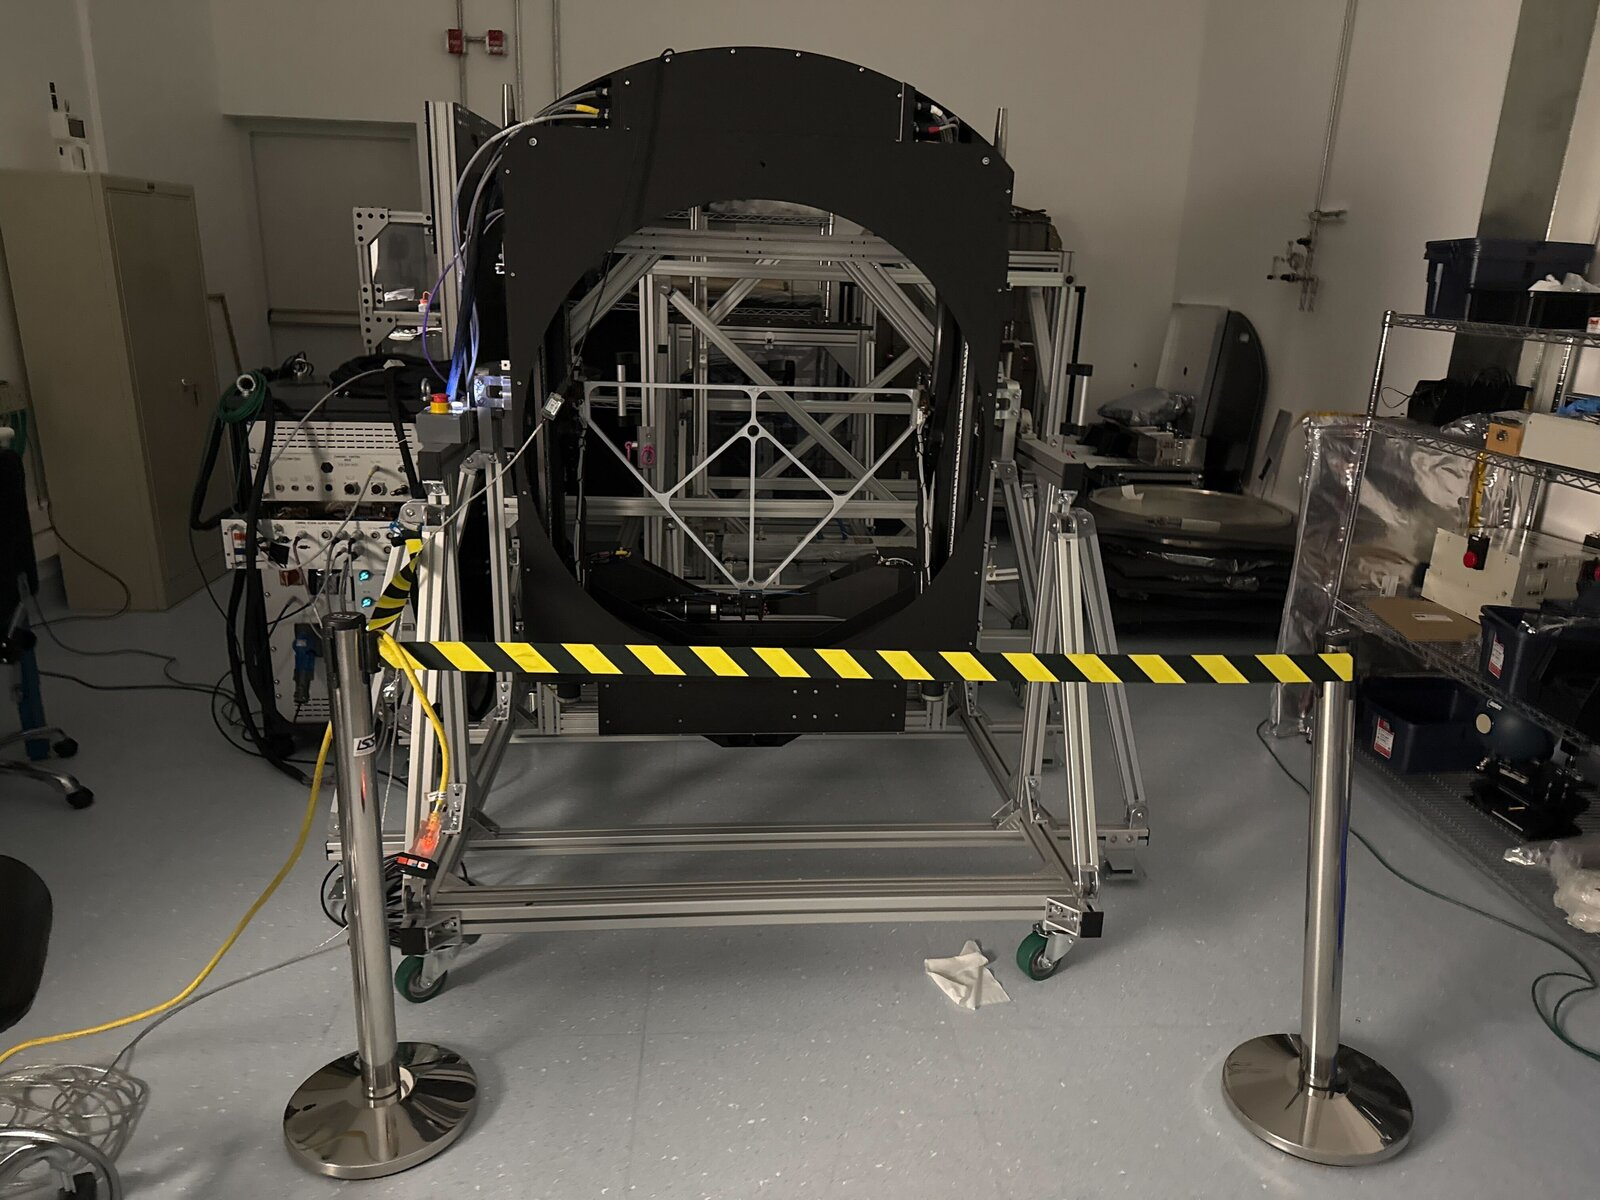
\includegraphics[height=4.98cm]{issues2025/figs/FES-03-a.jpg}\hfill
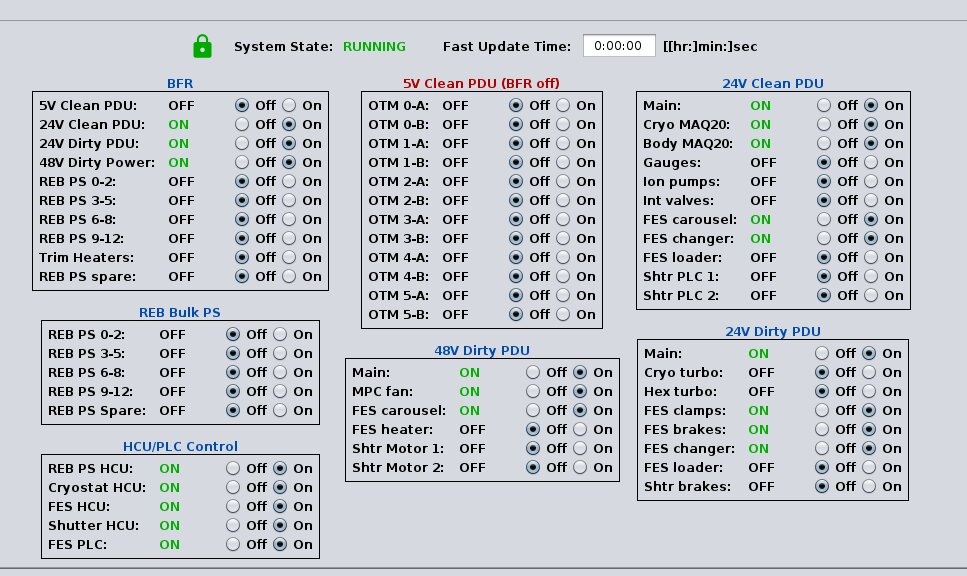
\includegraphics[height=4.98cm]{issues2025/figs/FES-03-b.jpg}
\caption{\textbf{FES-03.} Left: an autochanger on its stand in the clean room, where the homing procedure was qualified (2025-04-07).  Right: the quadbox power panel, whose FES carousel, clamp, loader and brake channels are the supplies behind the truck undervoltage faults (2025-02-13).}
\label{fig:iss-FES-03}
\end{figure}

\item[FES-04]\label{iss:FES-04} \textbf{Carousel controller position glitches and emergency stops.}
  \emph{First to last mention 2025-09-14 to 2026-04-14; status \textcolor{stopn}{\textbf{Open}}.}
  A rotation ends with the controller believing it has reached standby while it is somewhere else.  It starts on 2025 September~14 with a carousel that would not move on the first try (\rubintkt{LSSTCAM-129}), and the errors grow: $-8045\,\mu$m on December~13 --- together with a controller crash that was never explained --- then $+5019$ on 2026 March~11 (\rubintkt{OBS-1705}), $-$10187 on March~14, and on March~15 a following error of 32{,}767\,$\mu$m, which is exactly $2^{15}$, with the carousel bouncing off a limit at full speed (\rubintkt{OBS-1707}).  The carousel was run at 500\,rpm instead of 3400 until April~8.  The reading is a corrupted following-error value from the controller microcode, suspected to come from a protection added in November 2025.  What was changed on March~18 was the consequence and not the cause: the fault reaction was set to slow down rather than stop violently.  Rates measured afterwards did fall --- 5.92 to 3.95\,\% of rotations needing a recovery --- but Paris and the summit do not agree, and the working plan of May~25 still lists it as unfixed (\rubintkt{OBS-1853}).  A brake warm-up added in November 2025 as a mitigation had its own small consequence: it was not counted in the expected exchange time, and a filter change nearly timed out on 2026 January~7 until the limit was raised.

\item[FES-05]\label{iss:FES-05} \textbf{Loader 2 linear-table oil leak.}
  \emph{First to last mention 2026-06-19 to 2026-07-09; status \textcolor{stopn}{\textbf{Open}}.}
  Oil was found seeping from the vertical linear table of loader~2 on 2026 June~19, in the middle of a filter swap, which was canceled.  Cleaning did not stop it: the grease in the table has liquefied, and by early July the conclusion was that the table is full of oil.  Filter swaps have been done with a single loader and the filter storage box since, on a procedure written for the purpose.  The drain tap could not be opened --- the screw is locked, on the summit unit and on the prototype in Paris alike --- so the table could not even be emptied.  The repair under discussion, a new linear table, is a matter of months.

\item[FES-06]\label{iss:FES-06} \textbf{Carousel and autochanger deadlock on misaligned trucks.}
  \emph{First to last mention 2025-07-24 to 2025-07-30; status \textcolor{stres}{\textbf{Resolved}}.}
  On 2025 July~24 all filter-exchange motion froze at socket~3.  The autochanger trucks entered the clamp badly out of step --- 175 to 250\,$\mu$m apart --- and the two controllers then disagreed by construction, the carousel logic reading its sensors as an OR and the autochanger as an AND, so that neither would give way.  Recovery was mechanical: the camera was moved to horizontal and gravity released the jam.  A second jam followed on July~29 and needed an engineering-mode override; socket~3 was taken out of service until the October maintenance and a filter was removed for inspection, its pins found worn and replaced (\rubintkt{OBS-1130}, \rubintkt{OBS-1131}, \rubintkt{SUMMIT-11092}).  The friction that caused it was cured in October (FES-01) and the truck misalignment that made it worse in June 2026 (FES-03).

\item[FES-07]\label{iss:FES-07} \textbf{Autochanger relay wear from inclinometer glitches near zenith.}
  \emph{First to last mention 2025-04-28 to 2025-06-11; status \textcolor{stres}{\textbf{Resolved}}.}
  The autochanger's inclinometer glitches as it passes through the gravity null, and each glitch toggled the clamp relays; the relays are rated for of order 100{,}000 operations, so this was a wear-out risk rather than a fault.  It was raised in April 2025 and fixed by a PLC firmware update on June~9--11: ``The relays of the clamps should now stay quiet when the rotator reaches the inclinometer limit.''

\item[FES-08]\label{iss:FES-08} \textbf{Wake-up race leaving a filter reported unavailable.}
  \emph{First to last mention 2025-05-15 to 2025-06-15; status \textcolor{stopn}{\textbf{Open}}\,\textbf{?}.}
  Waking the carousel from power save could leave a socket's state unsettled, so that a filter present in the camera was reported as not available (\slactkt{LSSTCCSFCS-652}, \rubintkt{OBS-1004}).  The power-save and wake-up logic was reworked in version 8.2.0 of the filter-changer software in May 2025 and the fault appeared again in June, which says the rework did not cover it.  No closure is recorded.

\item[FES-09]\label{iss:FES-09} \textbf{Loader carrier overshoot at the handoff position.}
  \emph{First to last mention 2026-05-12 to 2026-05-25; status \textcolor{stopn}{\textbf{Open}}.}
  During the filter swap of 2026 May~12 the empty loader carrier reported itself on target at the handoff position and then overshot it by about 50\,$\mu$m, so the next command was rejected.  It was recovered by hand from the interface.  A ticket was opened for a proper plan (\rubintkt{LSSTCAM-177}) and the working plan of May~25 still lists it as a rare error to be fixed.  One occurrence.

\item[FES-10]\label{iss:FES-10} \textbf{Carousel wake-up with the standby probe and the socket sensor disagreeing.}
  \emph{First to last mention 2026-04-27 to 2026-05-07; status \textcolor{stopn}{\textbf{Open}}.}
  A carousel raised a not-at-standby alarm on 2026 April~27 although the sensor that reports whether a socket is empty disagreed with the standby probe after the wake-up.  A mechanism was proposed in early May and was not settled; the request at the end of the discussion was for a meeting rather than a fix.  It is a different failure from FES-04, which is a position error rather than a disagreement between two sensors.

\end{description}

\noindent\textit{Stray light}
\begin{description}
\item[OPT-01]\label{iss:OPT-01} \textbf{Stray-light HV bias trips.}
  \emph{First to last mention 2025-04-17 to 2025-10-22; status \textcolor{stwrk}{\textbf{Workaround}}.}
  Light reaching the focal plane with the shutter closed repeatedly tripped the HV bias: sunlight through an open P-flow door with the mirror covers open, head lamps and light past the filter-loader door during FES work, a laser tracker left running all day, dome floodlights during a public demonstration, dome lights switched on by accident (about 20 channels tripped, all ITL rafts), and specular reflection of the moon within roughly 20 degrees.  Each case produced a procedural rule --- mirror covers closed when the P-flow is open, a minimum moon-avoidance angle, HV off during dome-shutter and filter operations --- and the trips became less frequent, but the mechanism is unchanged.

\begin{figure}[H]
\centering
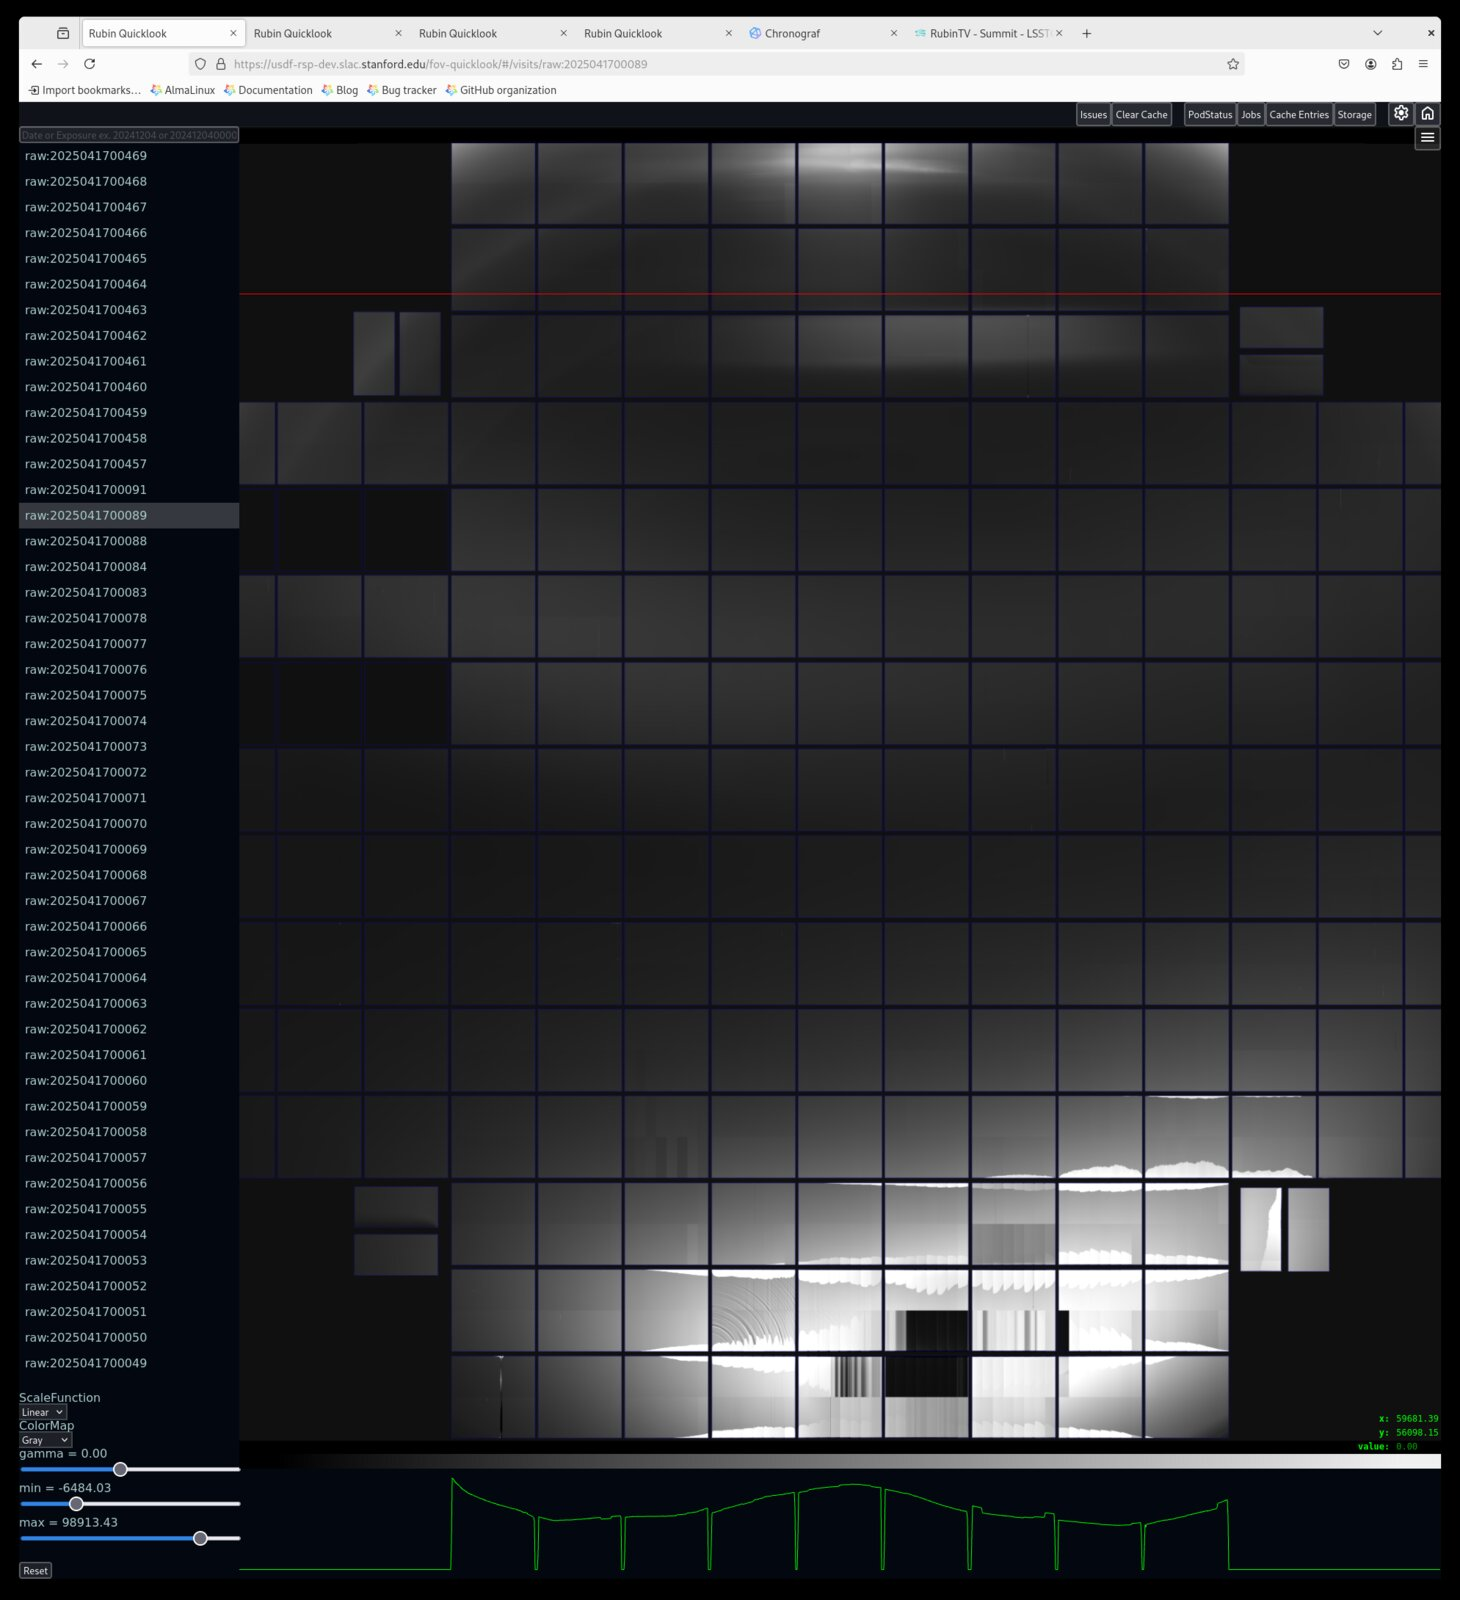
\includegraphics[height=6.19cm]{issues2025/figs/OPT-01-a.jpg}\hfill
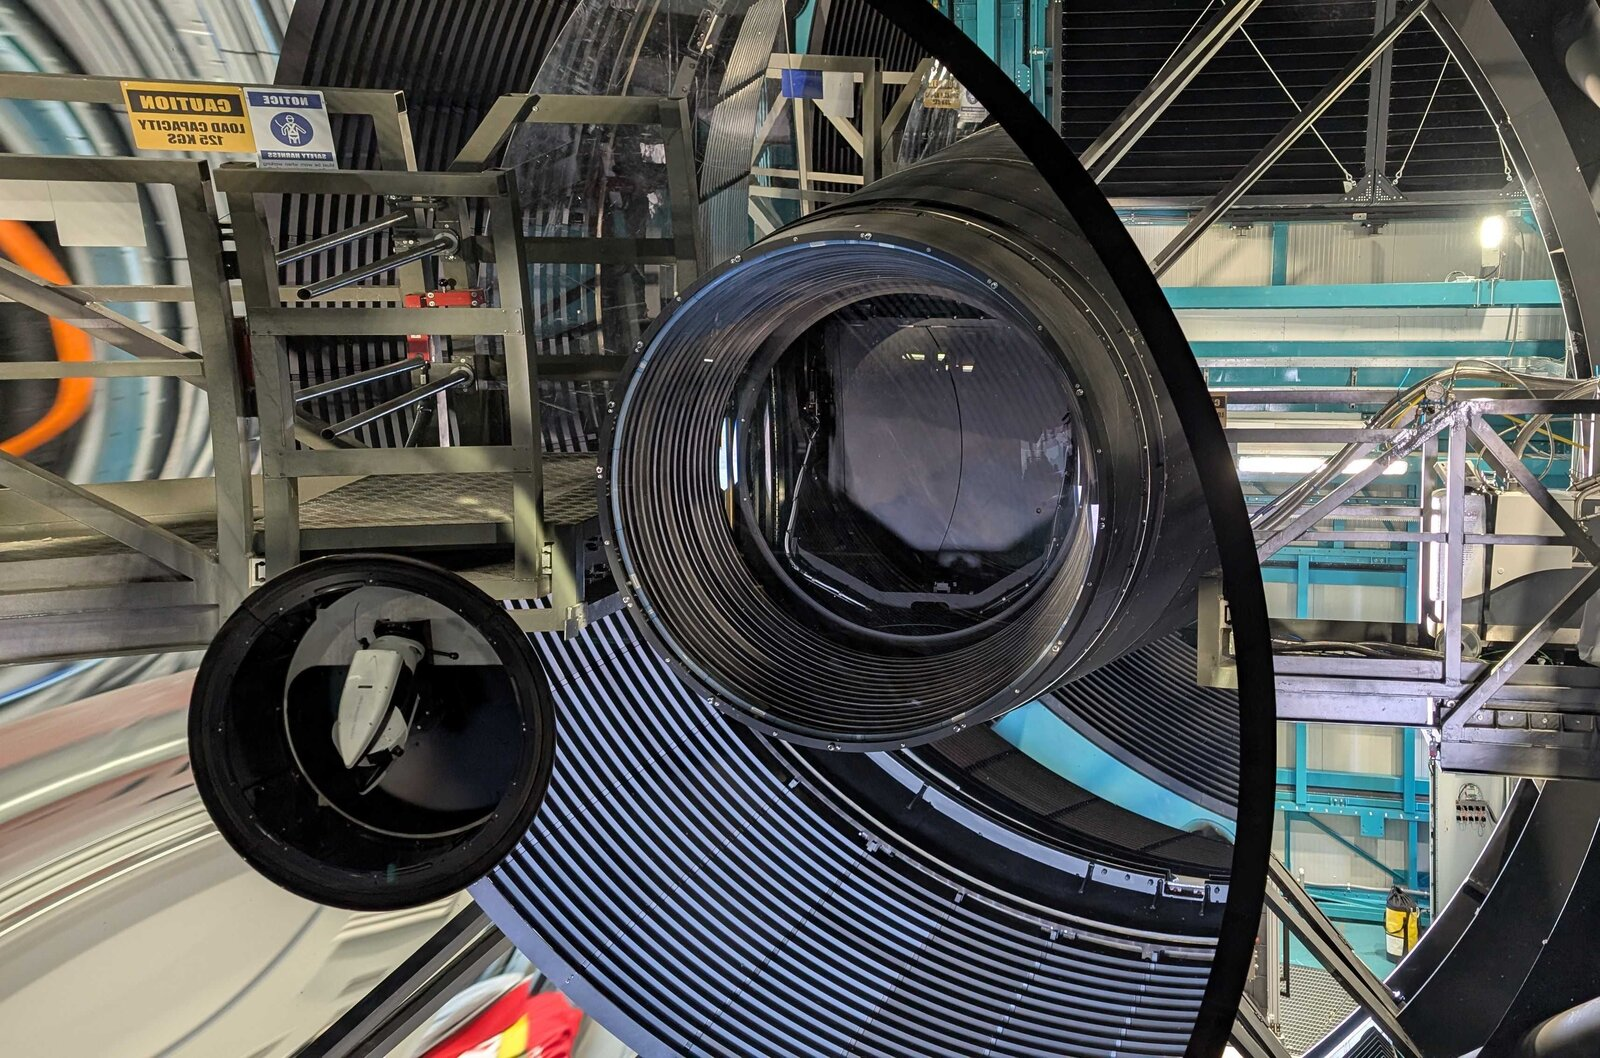
\includegraphics[height=6.19cm]{issues2025/figs/OPT-01-b.jpg}
\caption{\textbf{OPT-01.} Left: a focal-plane image taken while light was reaching the sensors with the shutter closed (2025-04-17).  Right: the camera and the open P-flow area on the day light through that route tripped the HV bias (2025-05-06).}
\label{fig:iss-OPT-01}
\end{figure}

\item[OPT-02]\label{iss:OPT-02} \textbf{``Banana'' stray-light feature in darks and flats.}
  \emph{First to last mention 2025-04-19 to 2025-04-20; status \textcolor{sttra}{\textbf{Transferred}}.}
  A banana-shaped feature appeared in dark and flat images, partly rotating with telescope azimuth and partly fixed, with equipment near M1M3 such as a laser tracker suspected as the source; reinstalling the pinhole filter was proposed as a partial mitigation for extended stray light.  No follow-up appears in either channel: the investigation was handed over to the stray-light group and is tracked there.

\begin{figure}[H]
\centering
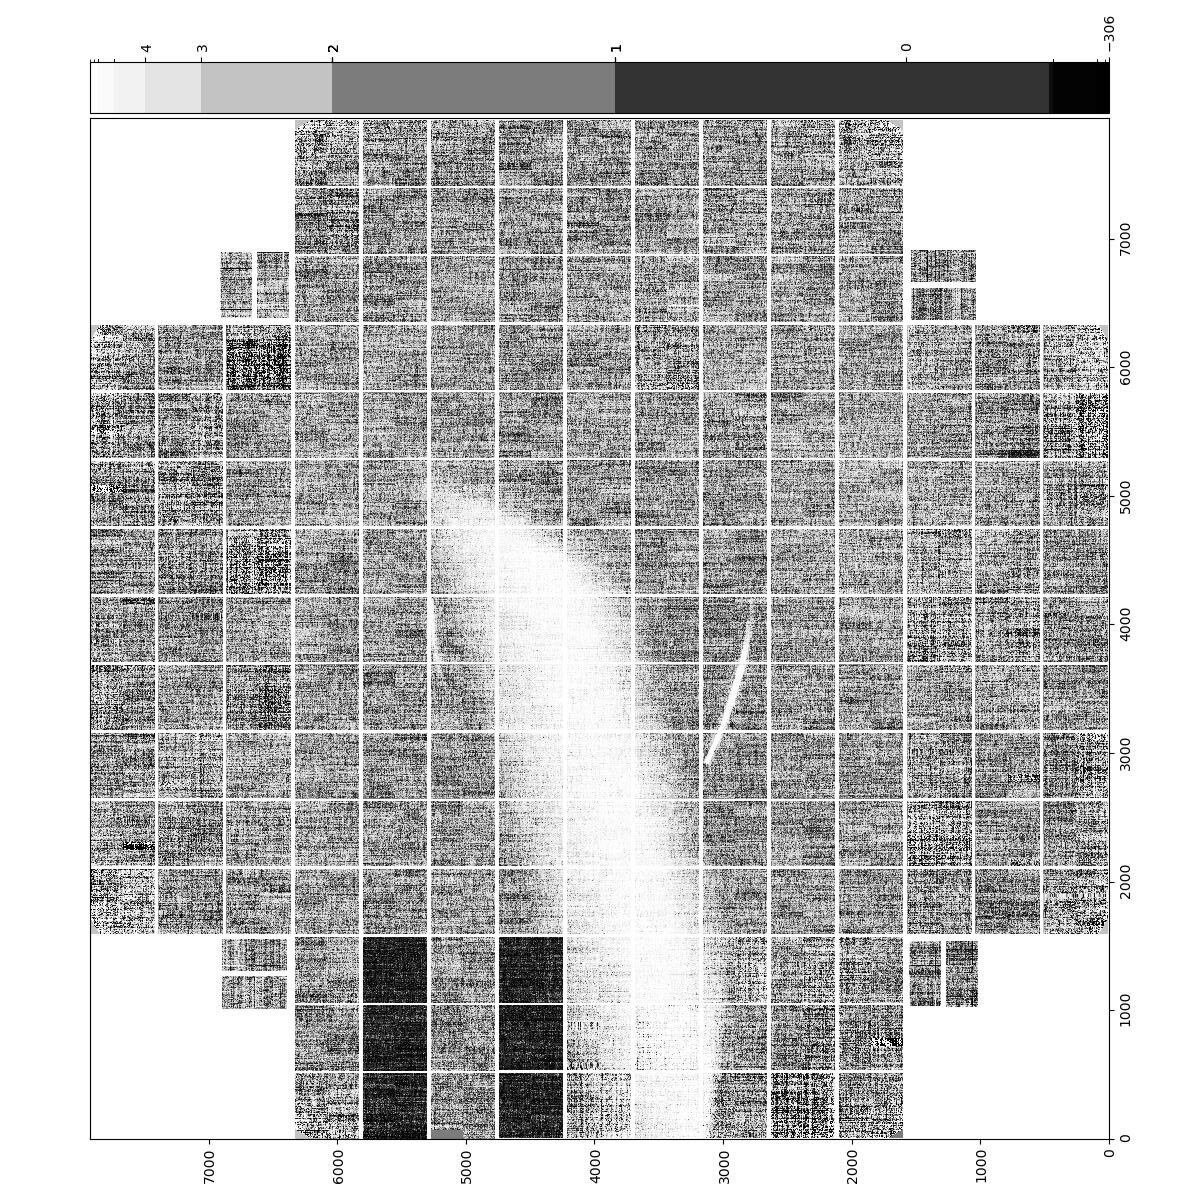
\includegraphics[height=6.50cm]{issues2025/figs/OPT-02-a.jpg}\hfill
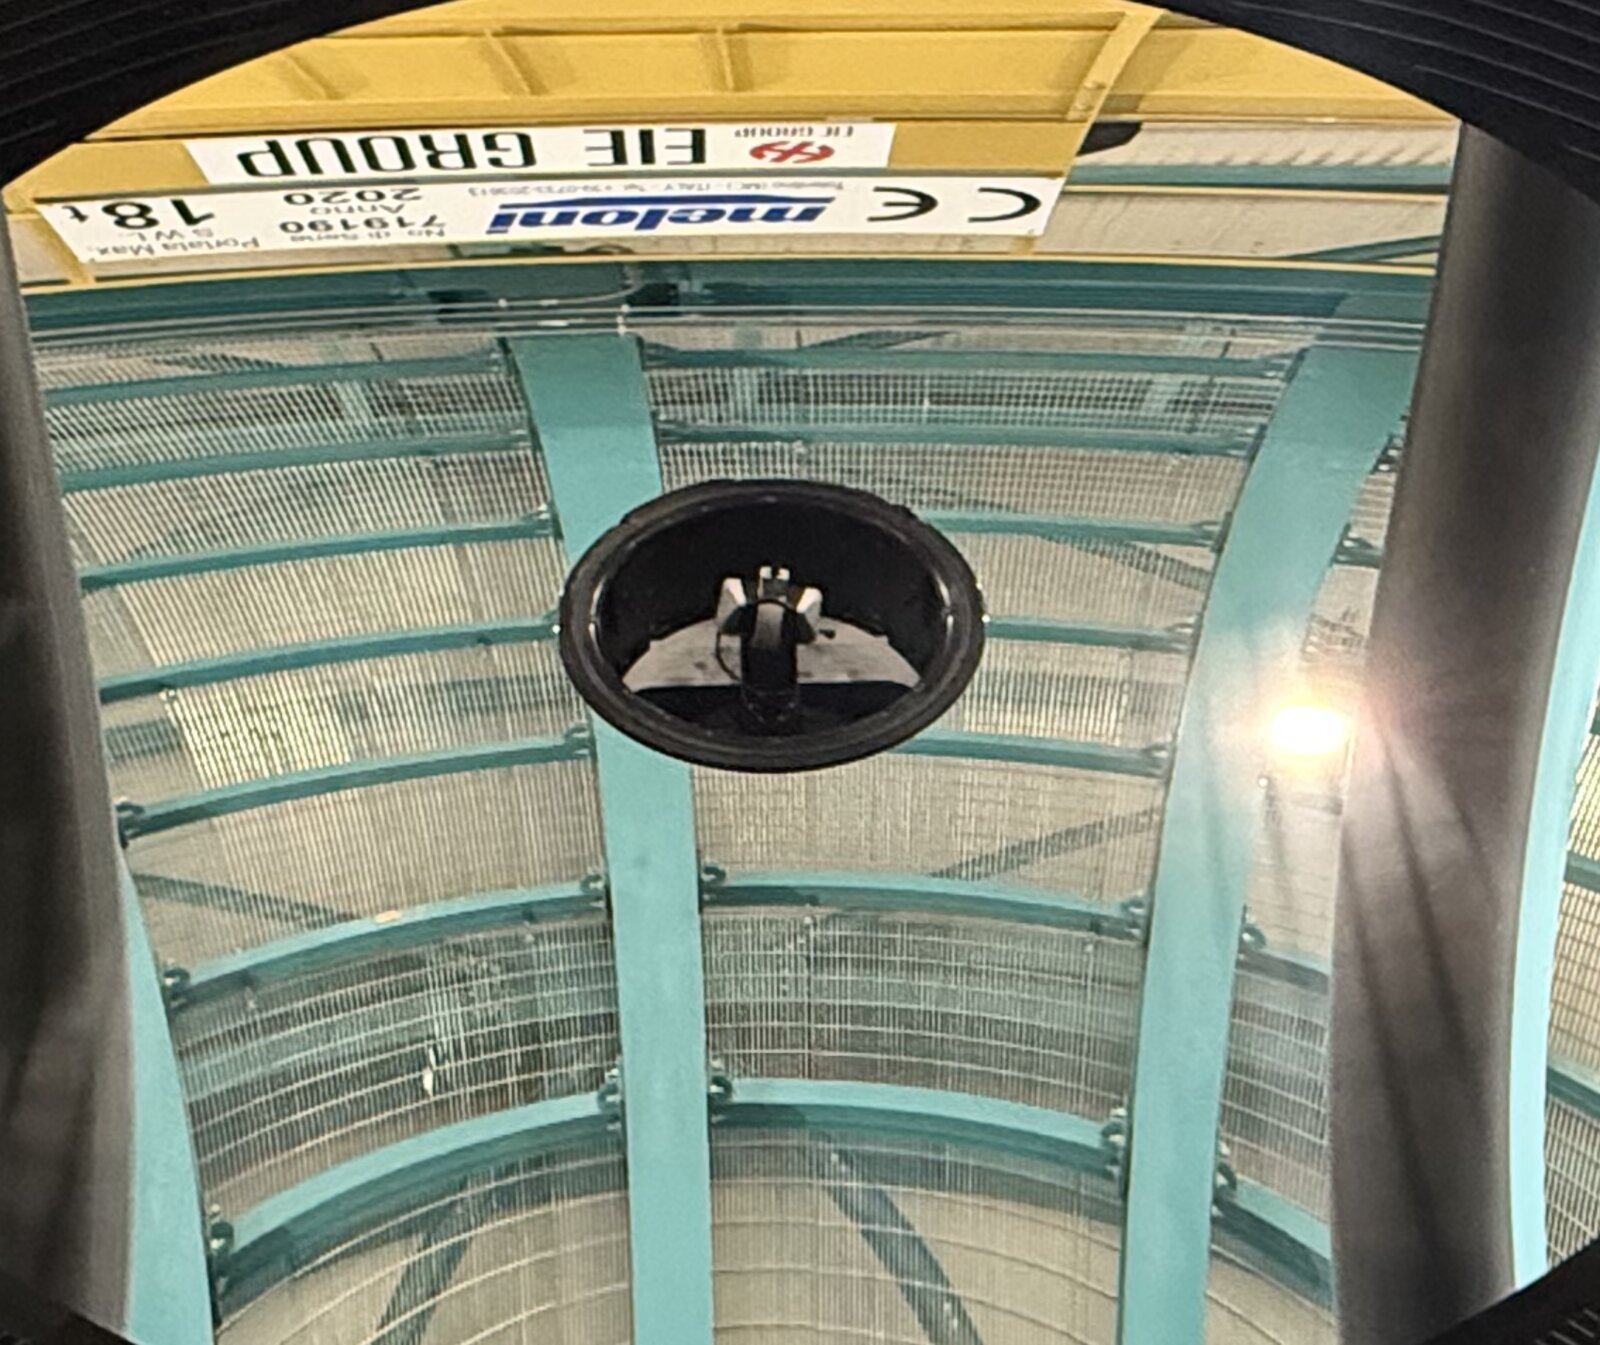
\includegraphics[height=6.50cm]{issues2025/figs/OPT-02-b.jpg}
\caption{\textbf{OPT-02.} Left: the banana-shaped feature in the focal plane that gave the issue its name.  Right: the dome interior photographed the same evening while looking for its source (2025-04-19, \#cam-operator).}
\label{fig:iss-OPT-02}
\end{figure}

\end{description}

\noindent\textit{Mechanical and integration}
\begin{description}
\item[MEC-01]\label{iss:MEC-01} \textbf{Sheared pancake-wrap bolts.}
  \emph{First to last mention 2025-01-28 to 2025-02-04; status \textcolor{stres}{\textbf{Resolved}}.}
  Several socket-head bolts holding the pancake wrap's central rotating assembly to the adapter plate sheared during the installation campaign and were found loose in the cable wrap.  The wrap was removed and rebuilt with new hardware at a reduced torque, and the interface was reworked (pin holes reamed, internal sliding blocks removed) in early February; a subsequent bolt test to 75\,ft-lb showed no failure.  The joint has given no trouble since and the item is treated as closed.

\begin{figure}[H]
\centering
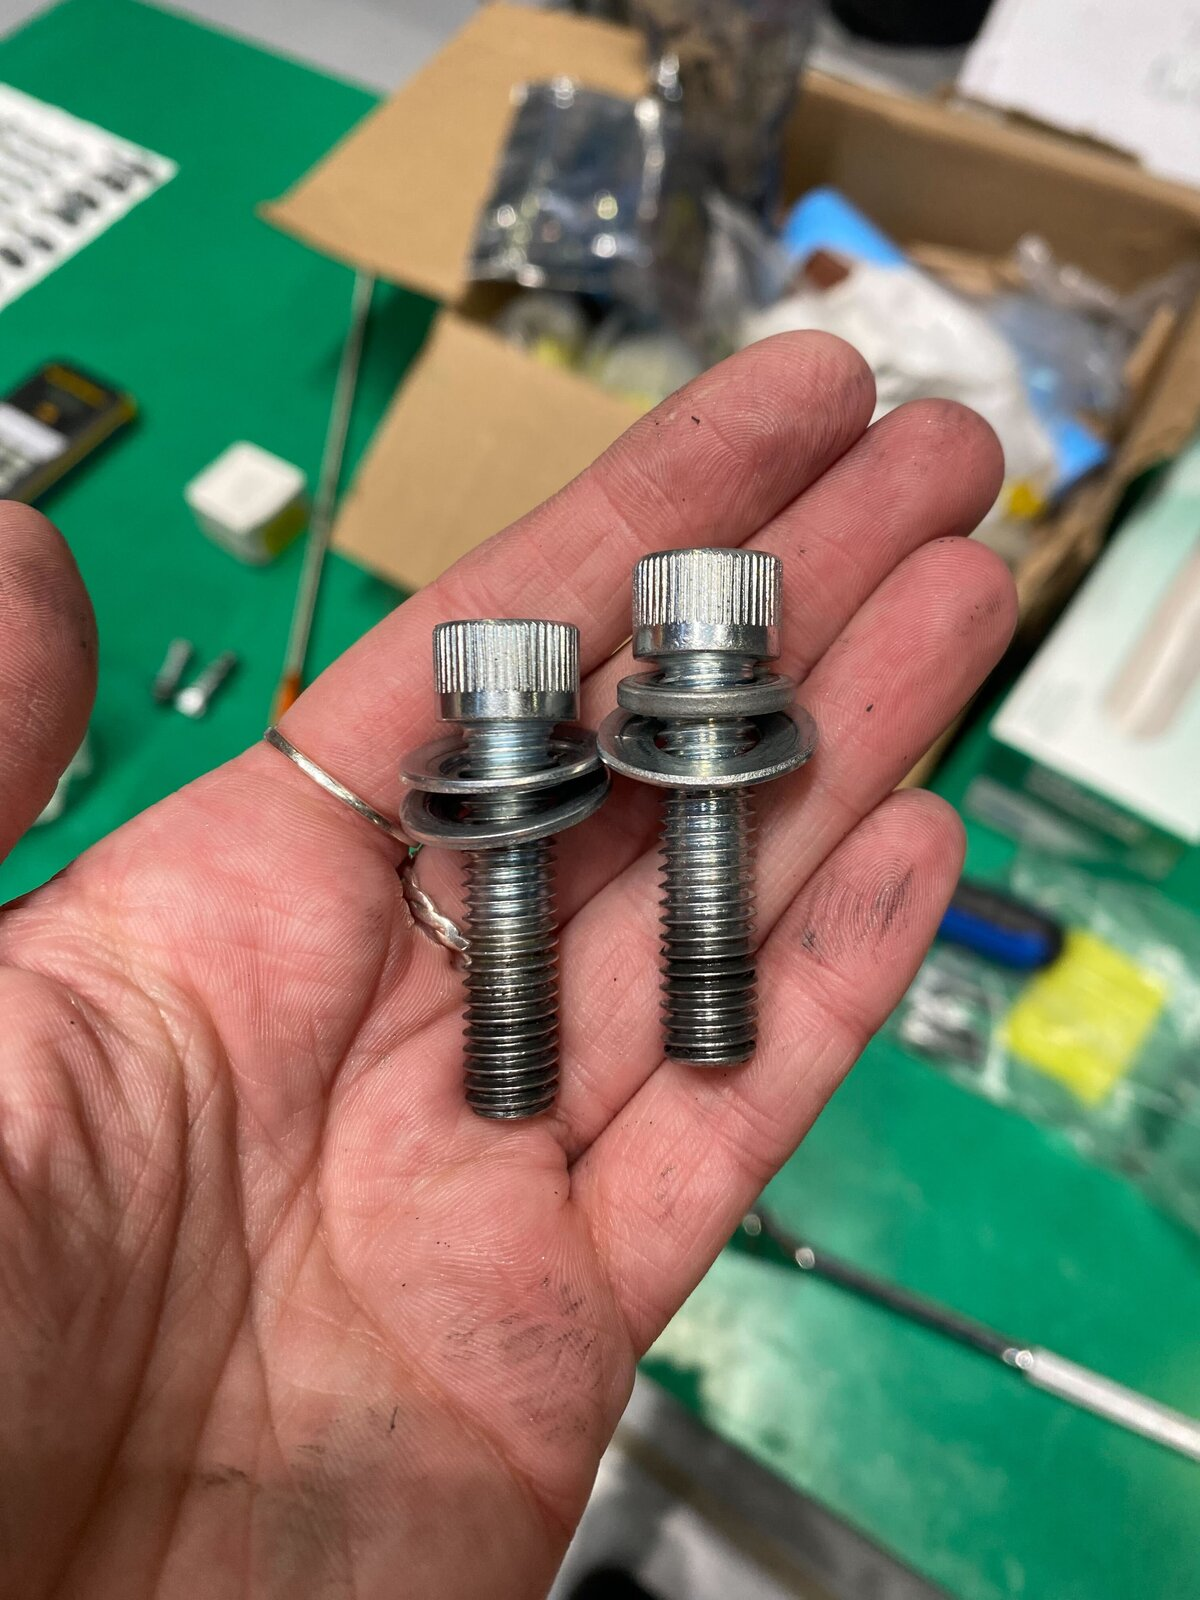
\includegraphics[height=6.50cm]{issues2025/figs/MEC-01-a.jpg}\hfill
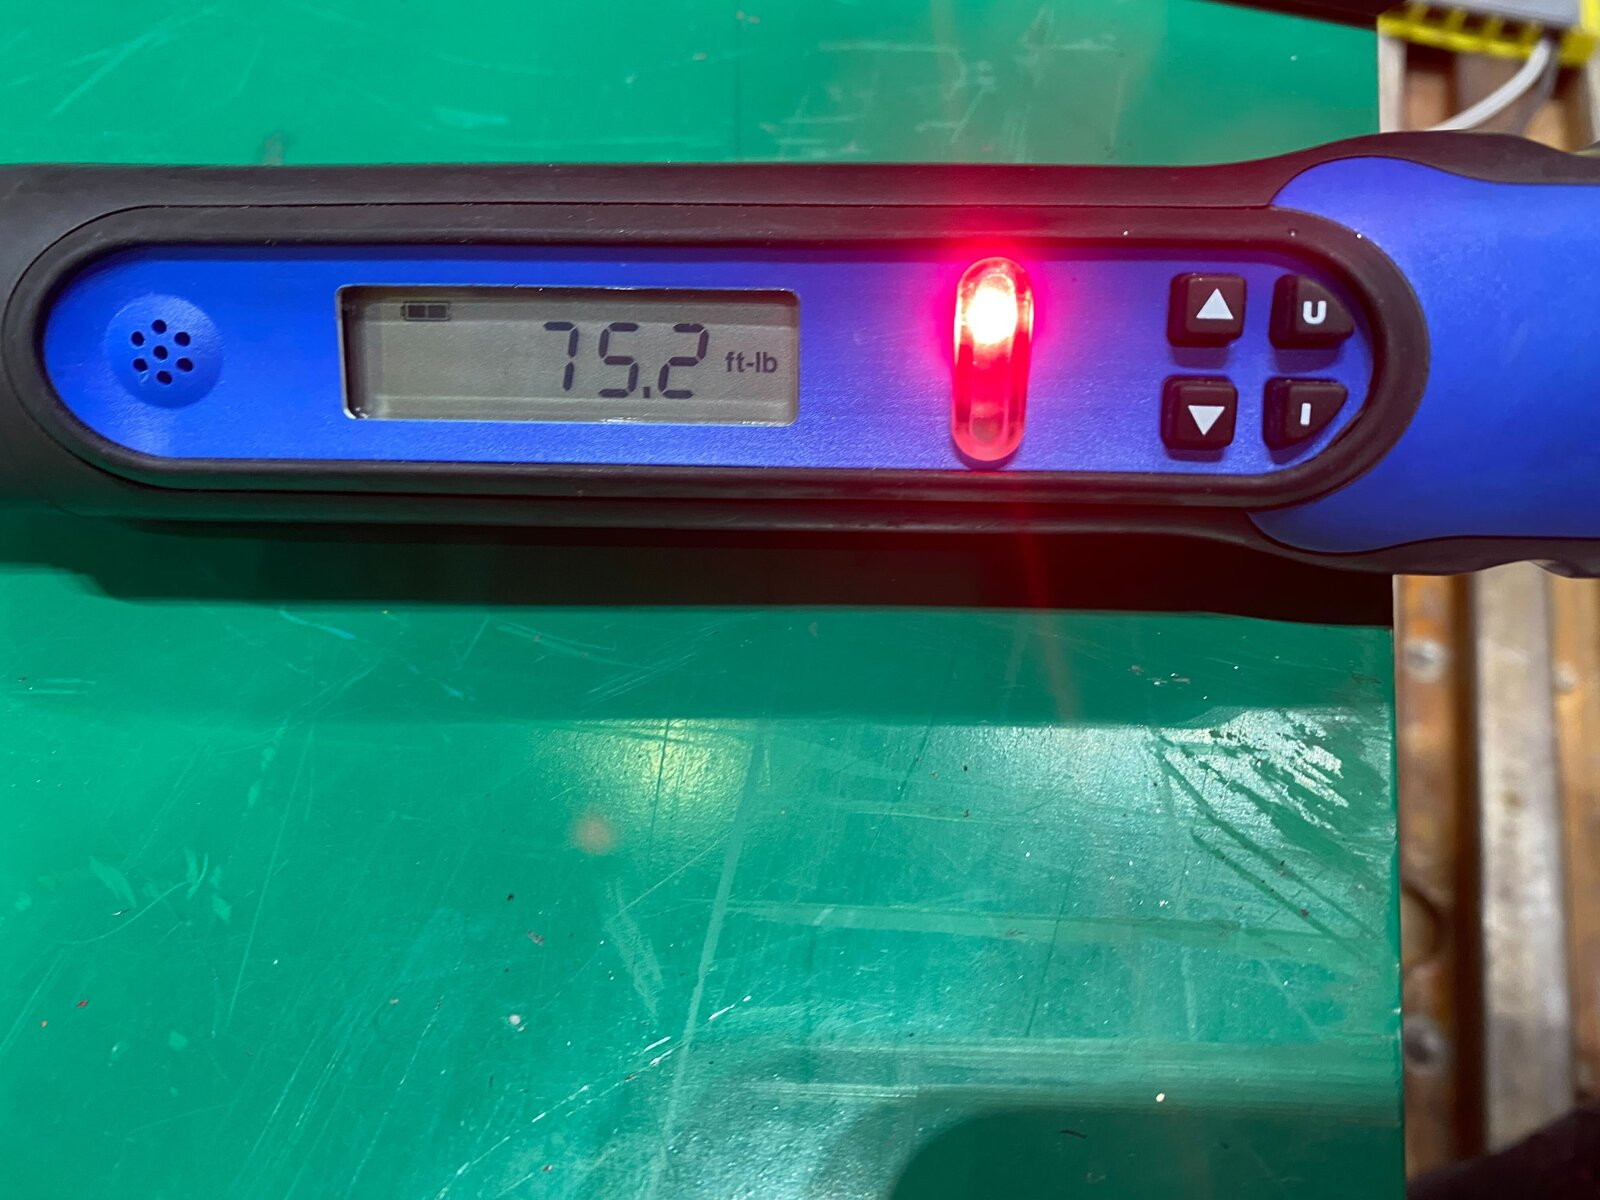
\includegraphics[height=6.50cm]{issues2025/figs/MEC-01-b.jpg}
\caption{\textbf{MEC-01.} Two of the sheared 3/8-16 socket-head bolts recovered from the cable wrap, and the bolt test that followed a few days later: 75.2\,ft-lb applied with no sign of failure (2025-01-30, \#cam-summit-ops).}
\label{fig:iss-MEC-01}
\end{figure}

\item[MEC-02]\label{iss:MEC-02} \textbf{Camera cable wrap interlock and telemetry faults.}
  \emph{First to last mention 2025-02-18 to 2025-10-09; status \textcolor{stopn}{\textbf{Open}}.}
  In February the cable-wrap local interlock at Level~3 was found to be entirely isolated from the rotator interlock, so the rotator would not stop on a cable-wrap fault, and the two were joined.  Since installation the wrap has instead blocked rotation: loss of its telemetry faulted the rotator in August (\rubintkt{OBS-1200}) and it stuck in a fault state during October maintenance rotations, recovered by bypassing the interlock at the mount engineering interface.  Described in the logs as a known issue.

\begin{figure}[H]
\centering
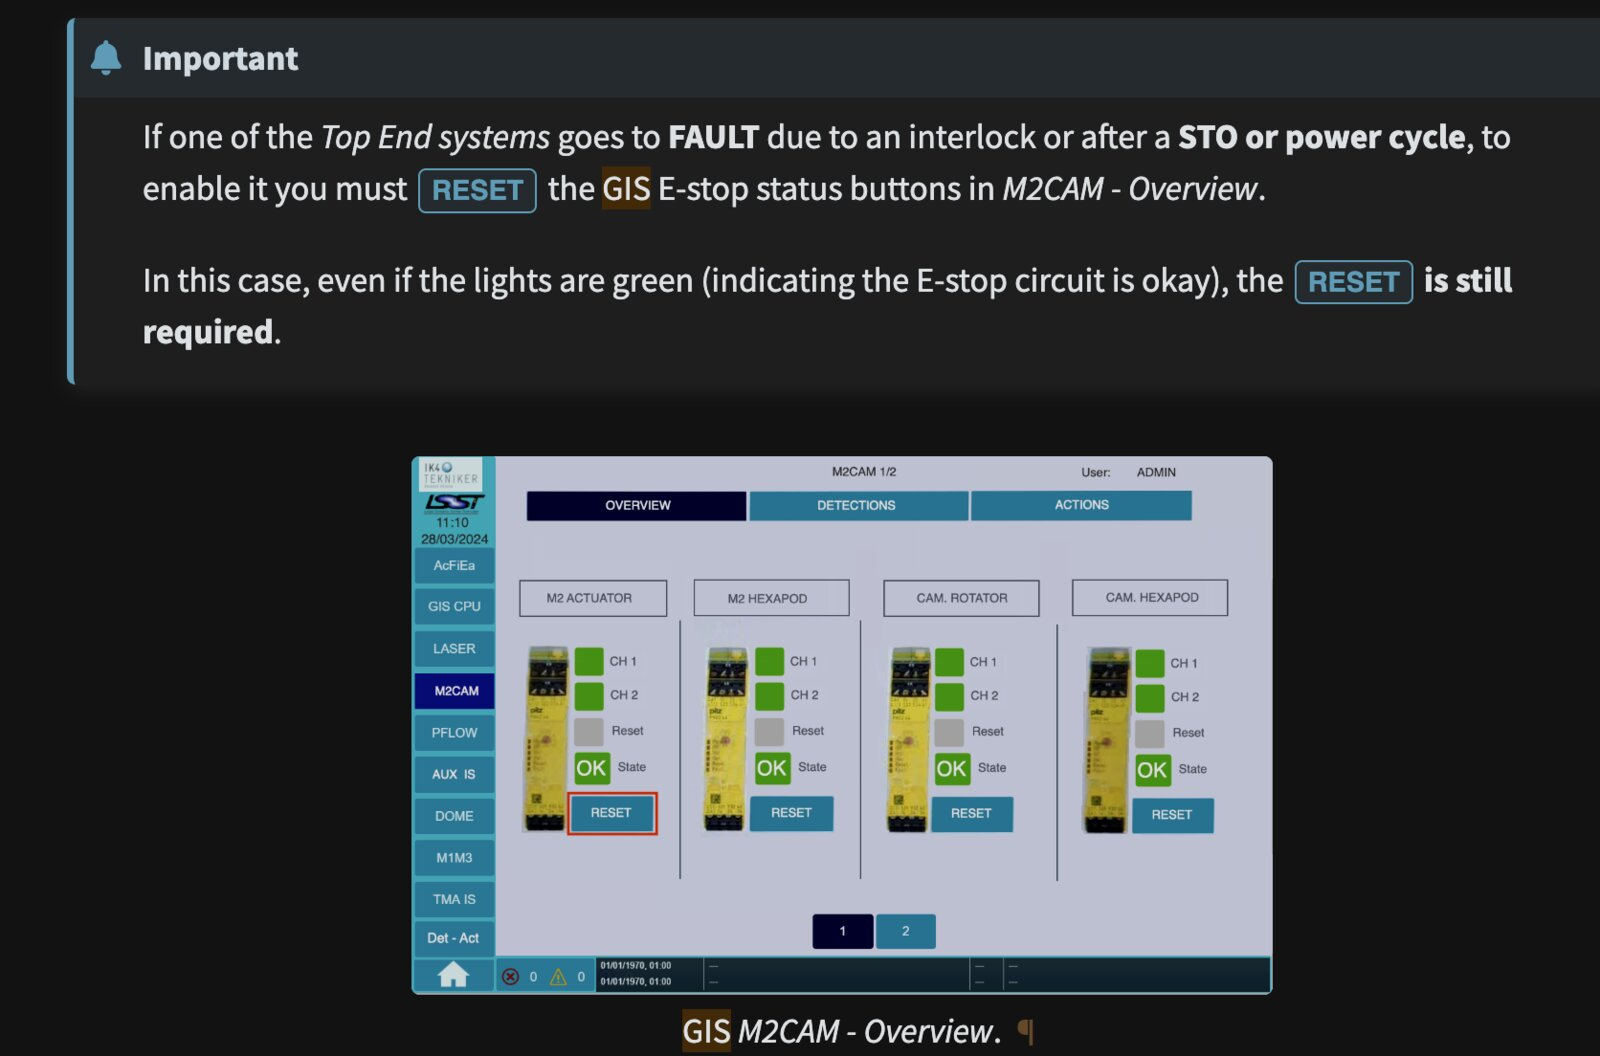
\includegraphics[height=5.27cm]{issues2025/figs/MEC-02-a.jpg}\hfill
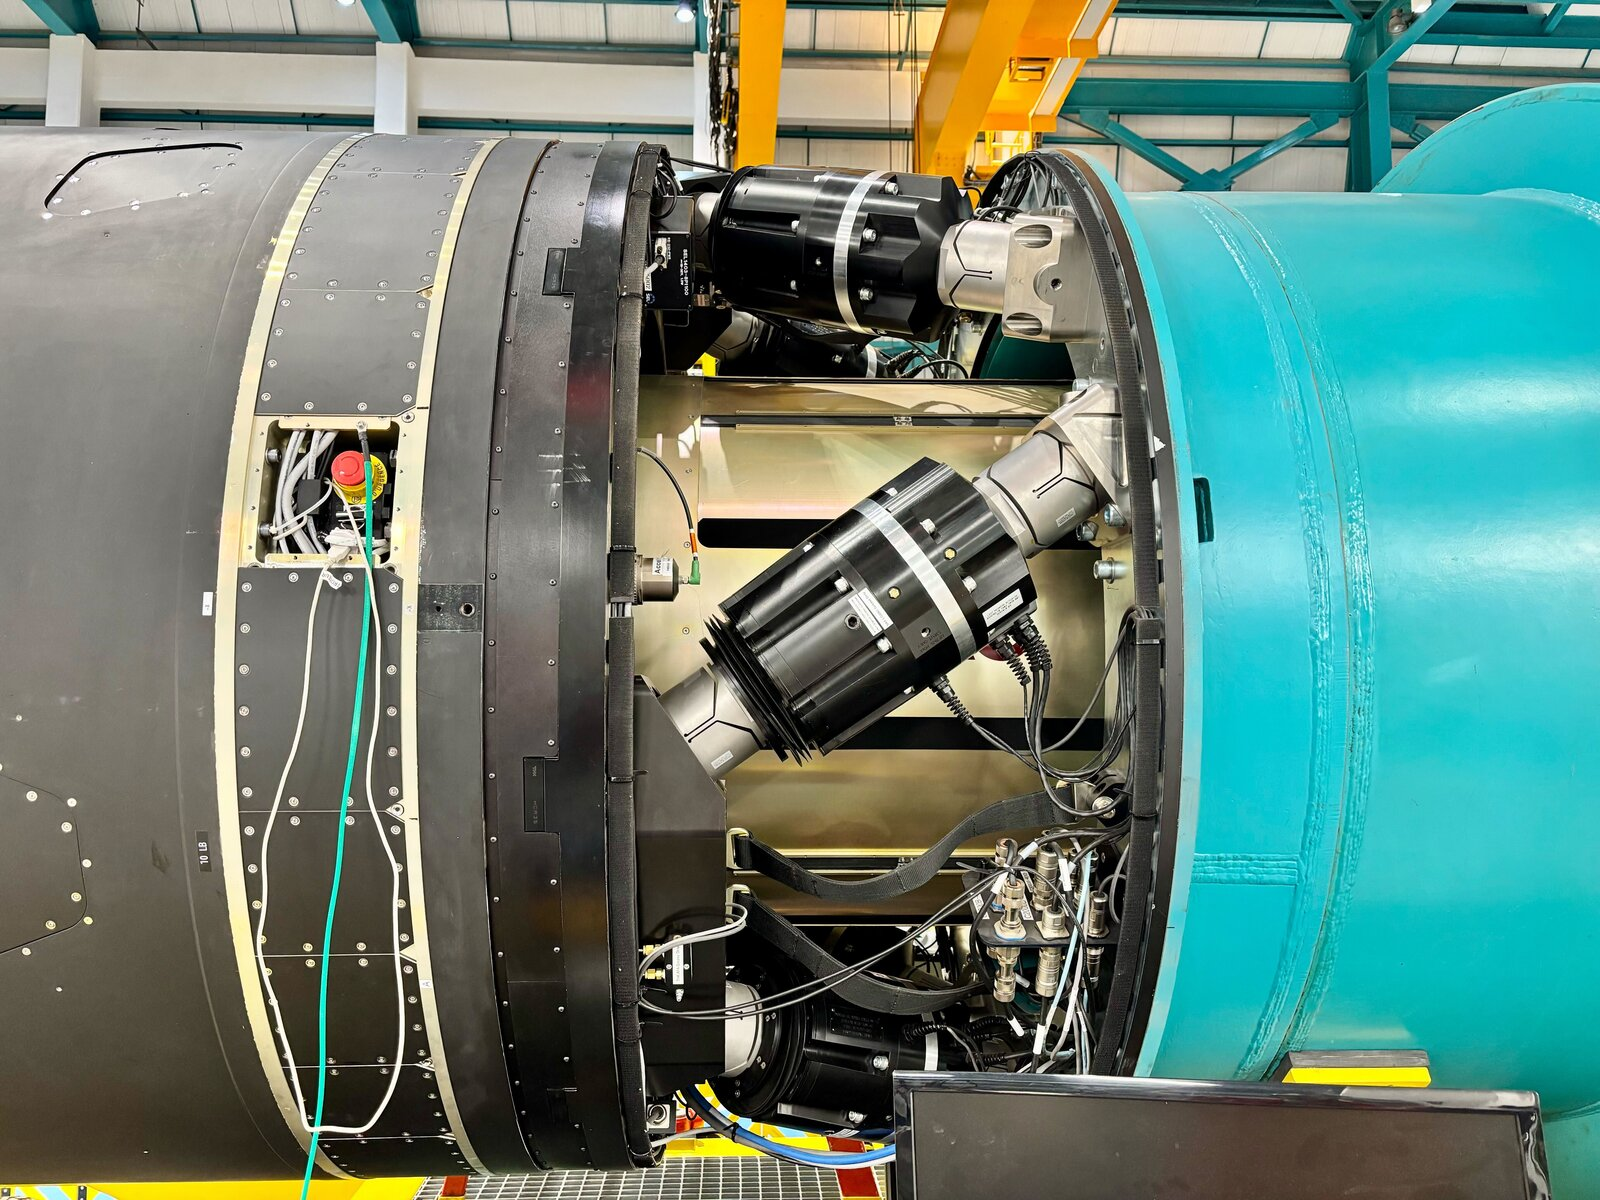
\includegraphics[height=5.27cm]{issues2025/figs/MEC-02-b.jpg}
\caption{\textbf{MEC-02.} Left: the operating note for the interlock, which has to be reset from the mount engineering interface after a fault or power cycle even when the status lights are green (2025-09-23).  Right: the camera rotator and cable-wrap region on the Top End Assembly (2025-03-03).}
\label{fig:iss-MEC-02}
\end{figure}

\item[MEC-03]\label{iss:MEC-03} \textbf{Creaking noise during large camera rotations.}
  \emph{First to last mention 2025-08-04 to 2025-09-07; status \textcolor{stopn}{\textbf{Open}}.}
  A repetitive clicking or creaking picked up by the camera shutter microphone, described as sounding like a Geiger counter.  It was first analyzed on August~4--5, when it appeared between 23:06:13 and 23:07:18\,UTC at 2--6\,kHz while the telescope was slewing: the M2 hexapod was found not to be moving but to be holding position with its actuator currents oscillating in a zigzag, which made it the first suspect.  On August~12 an alternative explanation --- the flapping straps of a temporary safety barrier on the mesh platform, blown by the HVAC fans and heard as the telescope slewed past --- was proposed and the straps were taped down.  The same sound returned on September~7 during 20-degree rotations every 3 minutes, which disproved the strap theory: this time the M2 hexapod was stationary while the camera hexapod moved with every rotation, though M2-hexapod motor currents still spiked at each one.  The recirculating ball bearings of the hexapod roller-screw actuators, or of the rotator, were then proposed as the source, and whether the sound has grown louder with age was raised and not answered.  A ticket was opened (\rubintkt{OBS-1158}) and nothing further appears in these channels.

\begin{figure}[H]
\centering
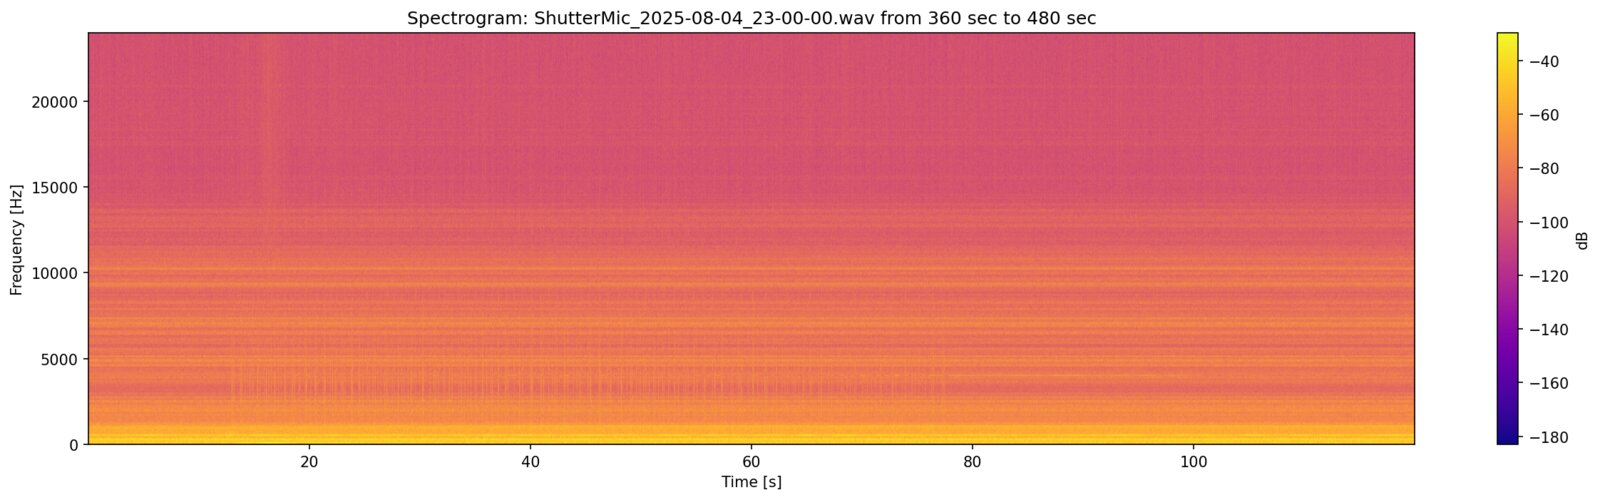
\includegraphics[width=0.90\textwidth]{issues2025/figs/MEC-03-a.jpg}
\\[4pt]
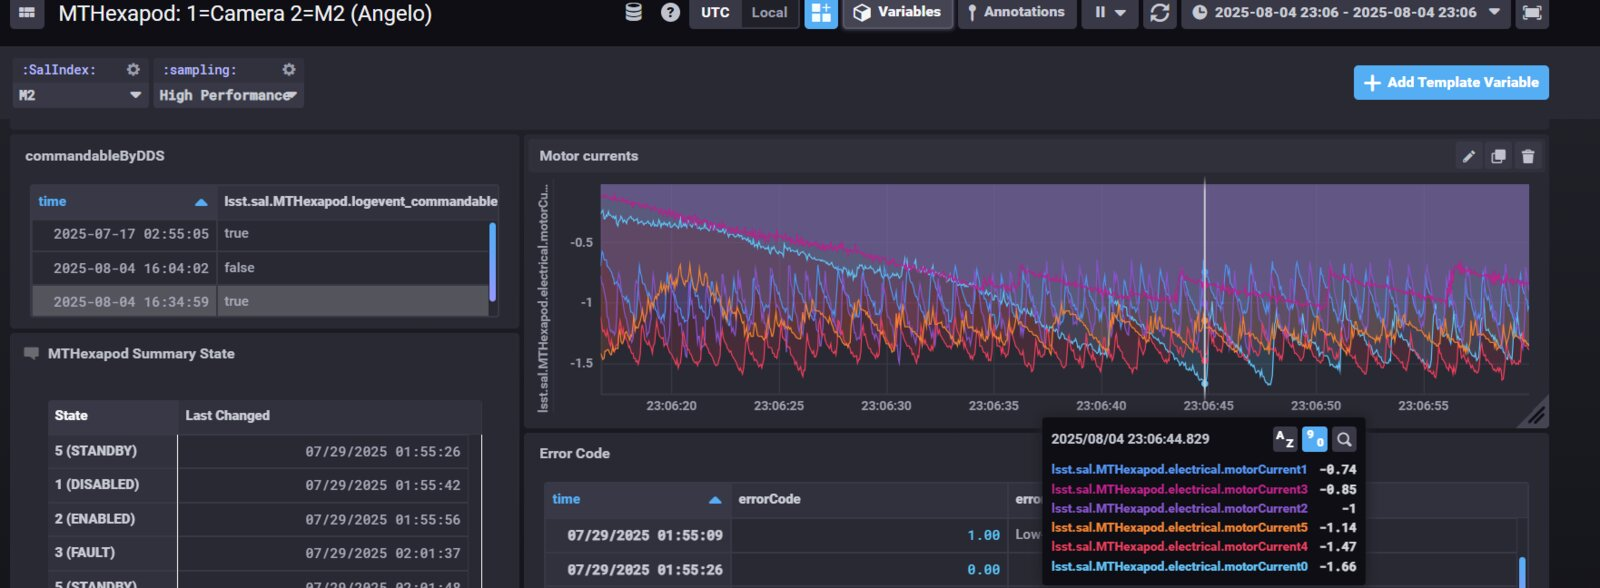
\includegraphics[width=0.90\textwidth]{issues2025/figs/MEC-03-b.jpg}
\caption{\textbf{MEC-03.} The August analysis.  Top: spectrogram of the shutter microphone recording of 2025-08-04, with the click visible as a vertical line across the band at about 18\,s into the excerpt.  Bottom: M2-hexapod telemetry for the same minute --- the hexapod is holding position, not moving, while its six actuator currents oscillate in the zigzag pattern that first made it the suspect (2025-08-05, \#cam-operator).  The September recurrence, which ruled out the safety-barrier explanation, is not illustrated here: the camera hexapod was the one moving then.}
\label{fig:iss-MEC-03}
\end{figure}

\item[MEC-04]\label{iss:MEC-04} \textbf{Electrostatic charging of the camera doors.}
  \emph{First to last mention 2025-01-21 to 2025-01-22; status \textcolor{stwrk}{\textbf{Workaround}}.}
  The camera doors ride on non-conductive tracks and are not electrically bonded, so they can charge as they slide; the temporary grounding wires used in the clean room had to be removed before the utility-trunk skins went on.  The accepted interim measure was an operational step to ground the doors by hand when opening or closing them.  A proper workaround using a grounding strap is being implemented.  The REB power-supply trips that motivated the concern are registered separately as FP-06.

\begin{figure}[H]
\centering
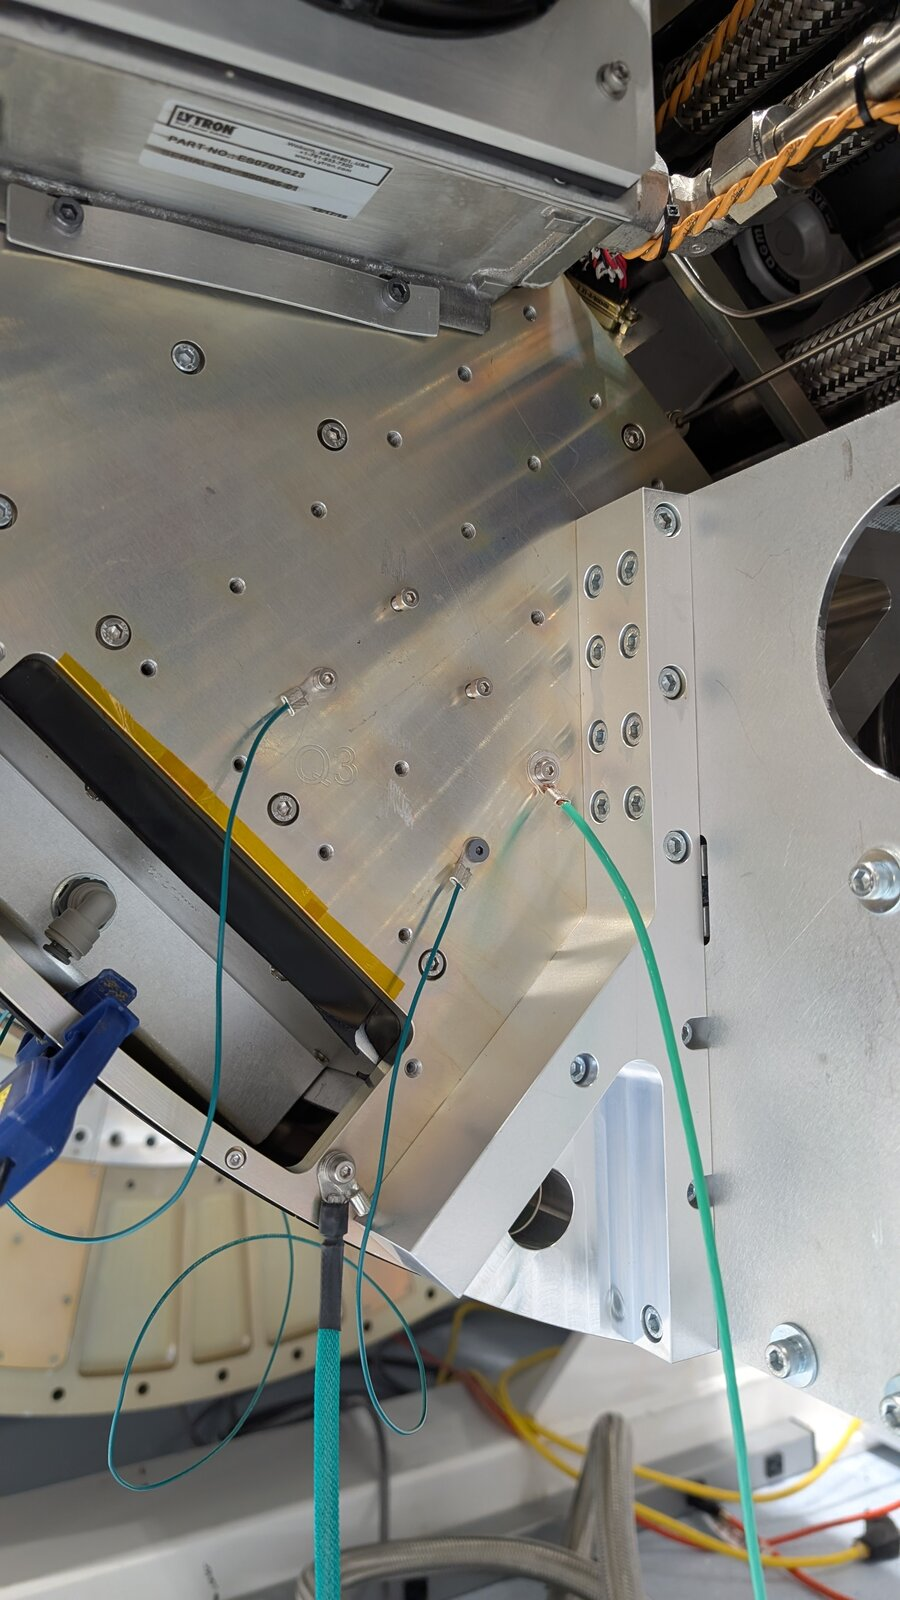
\includegraphics[height=6.41cm]{issues2025/figs/MEC-04-a.jpg}\hfill
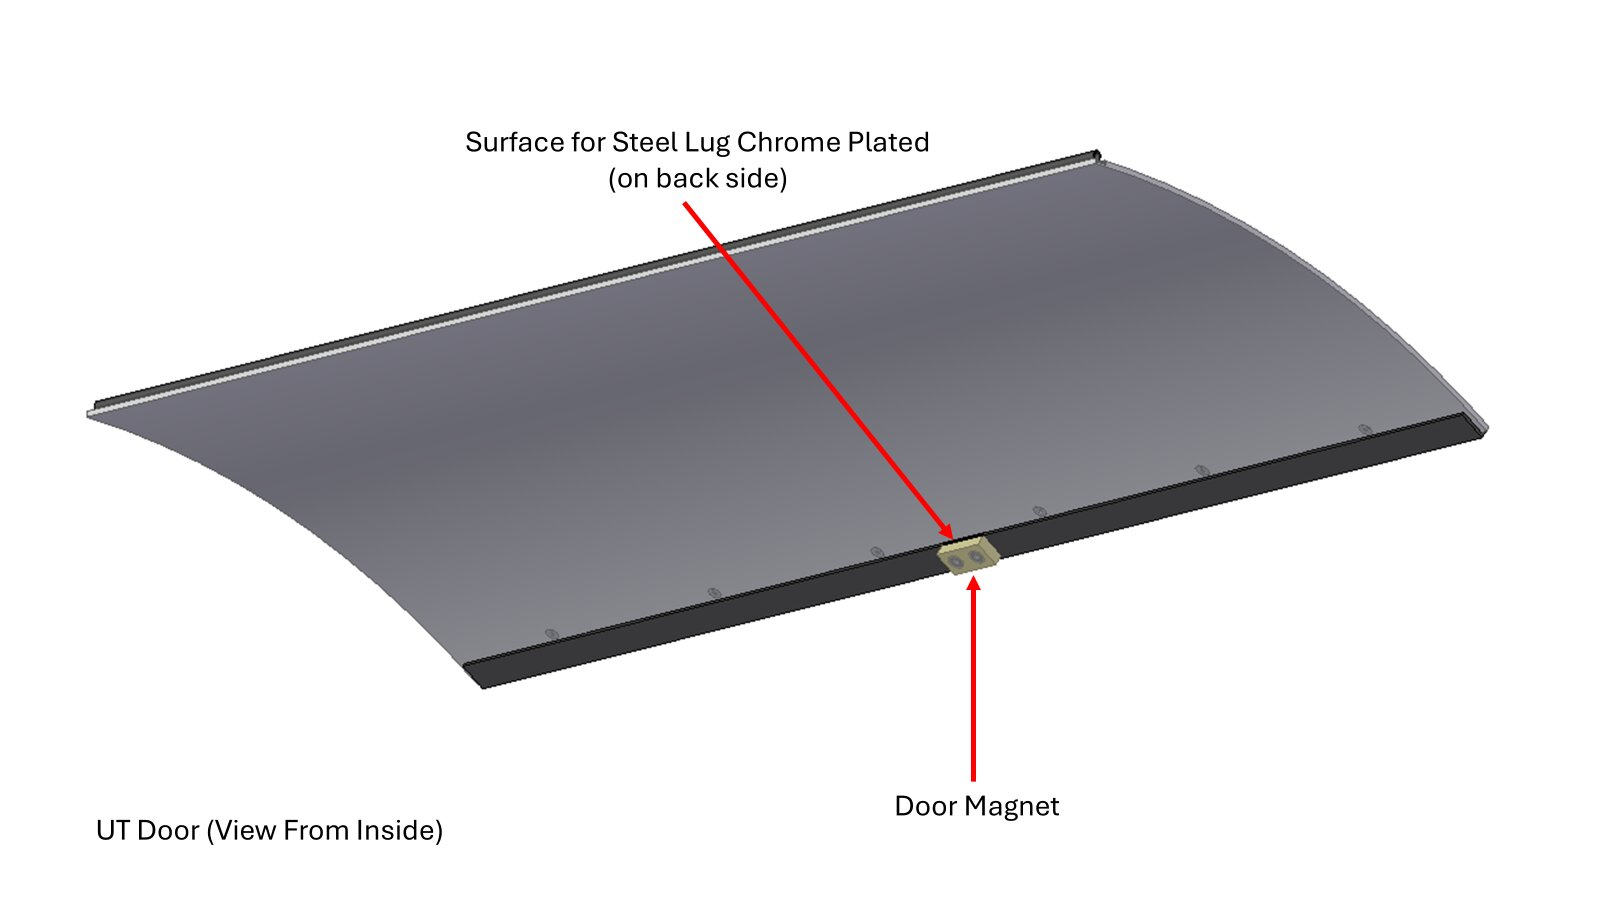
\includegraphics[height=6.41cm]{issues2025/figs/MEC-04-b.jpg}
\caption{\textbf{MEC-04.} Left: one of the temporary grounding wires used in the clean room, which had to come off before the utility-trunk skins were installed (2025-01-21).  Right: the utility-trunk door seen from inside, with the chrome-plated lug surface and the door magnet marked --- the interface a permanent grounding strap has to use (2025-01-21).}
\label{fig:iss-MEC-04}
\end{figure}

\end{description}

\noindent\textit{Summit IT}
\begin{description}
\item[IT-01]\label{iss:IT-01} \textbf{Collateral damage from summit OS and Kubernetes patching.}
  \emph{First to last mention 2025-02-06 to 2026-07-01; status \textcolor{stmit}{\textbf{Mitigated}}.}
  Roughly monthly summit patching costs the camera a day and a full reboot cascade across its servers, and has twice done real harm: in August a scripting error included the shutter HCU that was meant to be excluded and an authentication race condition then locked it out for hours --- judged serious because the same fault on a hardware-safety host would have been worse --- and in December the reboot coincided with a Dynalene outage.  The camera team's response was procedural: take the camera offline first, reboot in a defined order, verify link speeds and images before handing back.  The pattern held all through 2026: a patch or an upgrade lands, and something the camera needs goes with it --- control-system access during an urgent repair in January, a console panel broken by a user-interface release in May, a subsystem left unable to resolve a class after an upgrade in April.  Each was recovered in a day; the March server migration was the expensive one and is registered separately as IT-02.

\begin{figure}[H]
\centering
\begin{minipage}{\textwidth}
\hrule\vspace{4pt}
\begingroup\scriptsize
\begin{verbatim}
-- 2025-08-26 21:25--21:39 UTC, #cam-operator.  The shutter HCU had been rebooted by summit
-- patching that was supposed to exclude it.  The subsystem came back and kept producing
-- telemetry; nobody could log in to it.

lsstcam-vw02$ ssh lsstcam-shutter01.cp.lsst.org
Connection closed by UNKNOWN port 65535

$ nmap -p 22 lsstcam-shutter01.cp.lsst.org
Host is up (0.023s latency).
PORT   STATE SERVICE
22/tcp open  ssh

$ ssh lsstcam-shutter01
The authenticity of host 'lsstcam-shutter01' can't be established.
ED25519 key fingerprint is SHA256:enI61SsU+a9SGdEwIPkAF5LfqhOwTDvi8xLylPPZEMk.
Are you sure you want to continue connecting (yes/no/[fingerprint])? yes
Server host/lsstcam-shutter01.cp.lsst.org@LSST.CLOUD not found in Kerberos database
\end{verbatim}
\endgroup
\vspace{-10pt}\hrule
\end{minipage}
\caption{\textbf{IT-01.} Patching collateral damage at its most awkward: the host is up, the port is open, the subsystem is running and sending telemetry, and the camera team is locked out of it for hours by an authentication race.  The shutter was not used until access was restored.  The same fault on a host carrying hardware protection would have been considerably worse, which is why this entry is kept.}
\label{fig:iss-IT-01}
\end{figure}

\item[IT-02]\label{iss:IT-02} \textbf{Server migration and the lsstcam-mcm1 crashes.}
  \emph{First to last mention 2026-03-04 to 2026-03-27; status \textcolor{stwrk}{\textbf{Workaround}}.}
  The March 2026 migration moved the CCS database from \texttt{db01} to \texttt{db02}, renamed the data-collection nodes and moved the master control machine to \texttt{mcm1}.  The new machine crashed repeatedly from March~25, once wedging the lock manager and the guider in the middle of an observation, and hardware diagnostics found nothing; the team reverted to the original host on March~27 and left \texttt{mcm1} with IT.  The renaming also broke tooling and documentation for weeks.  A contributing defect was found on the way: the lock manager persists its state when a lock is taken and at shutdown, but not when one is released.

\end{description}

\noindent\textit{Cryostat vacuum}
\begin{description}
\item[VAC-01]\label{iss:VAC-01} \textbf{Cryostat vacuum.}
  \emph{First to last mention 2026-01-27 to 2026-02-16; status \textcolor{sttra}{\textbf{Transferred}}.}
  After the warm-up and cool-down of January 2026 the cryostat did not come back to the pressure it had held before.  A leak at a feedthrough was located and sealed, and the camera returned to the observatory control system on February~16 after 17 days off sky.  Cryostat vacuum performance has been followed closely since; it is treated in a separate note and is not carried further here.

\item[VAC-02]\label{iss:VAC-02} \textbf{Pump cart and vacuum gauge reliability.}
  \emph{First to last mention 2026-05-05 to 2026-06-25; status \textcolor{stwrk}{\textbf{Workaround}}.}
  Vacuum work in 2026 was slowed repeatedly by the equipment it depends on.  A bent pin in the pump cart's RS232 connector dropped the serial link on May~5 and closed the gate valves; the same connector failed again on June~21--22, driving the camera to a safe state, and was recovered only by power-cycling the cart with no cause identified.  The cart's secondary pump will not start below about 6--8\,$^{\circ}$C, which held up planned vacuum work on several days in June until the heater blanket was fitted again.  Separately the heat-exchanger vacuum gauge intermittently reports a stale combined reading instead of switching to its cold-cathode value, and has to be power-cycled by hand; that is a gauge firmware defect and recurred in March and June.

\end{description}

\paragraph{Scope of these judgements.}
An issue is called open when the channels record no resolution, whether or not
it was still being discussed in July 2026; that is a statement about the record,
not proof that nothing was done.  Statements of cause are those recorded in the
channels at the time.  The record stops on 13~July 2026, when the summit was
closed ahead of the storm.  The camera was safed and warmed over the following
three days and was still off sky in September; the storm, the damage and the
recovery are a separate document, and nothing after 13~July is registered here.

